\documentclass[12pt, a4paper]{article}

% 基礎套件
\usepackage[margin=2.5cm]{geometry}
\usepackage{xeCJK} % 支援中文
\usepackage{graphicx}
\usepackage{listings}
\usepackage{xcolor}
\usepackage{booktabs}
\usepackage{longtable}
\usepackage{hyperref}
\usepackage{float}

% 設定字體 (Windows 下常用的字體)
\setCJKmainfont{Microsoft JhengHei}[
    AutoFakeBold=2.5,
    AutoFakeItalic=true
]

% 設定程式碼樣式
\definecolor{codegreen}{rgb}{0,0.6,0}
\definecolor{codegray}{rgb}{0.5,0.5,0.5}
\definecolor{codepurple}{rgb}{0.58,0,0.82}
\definecolor{backcolour}{rgb}{0.95,0.95,0.92}

\lstset{
    language=VHDL,
    backgroundcolor=\color{backcolour},   
    commentstyle=\color{codegreen},
    keywordstyle=\color{magenta},
    numberstyle=\tiny\color{codegray},
    stringstyle=\color{codepurple},
    basicstyle=\ttfamily\small,
    breakatwhitespace=false,         
    breaklines=true,                 
    captionpos=b,                    
    keepspaces=true,                 
    numbers=left,                    
    numbersep=5pt,                  
    showspaces=false,                
    showstringspaces=false,
    showtabs=false,                  
    tabsize=2,
    frame=single
}

\title{微處理器系統實驗報告 - Lab 05 \\ \Large 移位萬用暫存器 (Shift Universal Register)}
\author{第 19 組 \\ 資工二 \\ 113590051 楊承諭、113590017 黃楷程}
\date{2026年5月13日}

\begin{document}

\maketitle
\newpage

\section{實驗內容}
本次實驗目標是設計一個 \textbf{10位元移位萬用暫存器 (N-bit Shift Universal Register)}。該暫存器需具備以下功能：
\begin{enumerate}
    \item \textbf{同步清除 (Synchronous Clear)}：當 \texttt{clean} 訊號為高電位時，在時脈正緣觸發下清空暫存器內容。
    \item \textbf{平行載入 (Parallel Load)}：當 \texttt{load} 訊號為高電位時，將 10 位元的平行輸入 \texttt{di} 載入至暫存器。
    \item \textbf{左移/右移 (Left/Right Shift)}：透過 \texttt{lr\_sel} 選擇位移方向。
    \begin{itemize}
        \item \texttt{lr\_sel = '1'}：左移，並將串列輸入 \texttt{sdi} 補入 LSB。
        \item \texttt{lr\_sel = '0'}：右移，並將串列輸入 \texttt{sdi} 補入 MSB。
    \end{itemize}
    \item \textbf{輸出顯示}：透過 10 顆 LED 燈 (\texttt{qo}) 即時顯示暫存器內部的數值。
\end{enumerate}

透過此實驗，我們掌握了 VHDL 中 \texttt{GENERIC} 的用法、\texttt{process} 內的同步控制邏輯，以及如何使用 \texttt{for loop} 簡化移位操作。

\section{實驗過程及結果}

\subsection{實驗過程}
\begin{enumerate}
    \item \textbf{程式撰寫}：編寫 \texttt{N\_bit\_DFF.vhd}，使用 Behavioral 模型描述暫存器邏輯。其中使用了 \texttt{rising\_edge(clk)} 確保所有動作皆在時脈正緣觸發。
    \item \textbf{腳位分配}：
    \begin{itemize}
        \item \texttt{clk} 分配至 \texttt{PIN\_M23} (KEY0)。
        \item \texttt{clean} 分配至 \texttt{PIN\_AB23} (SW12)。
        \item \texttt{load} 分配至 \texttt{PIN\_AC24} (SW10)。
        \item \texttt{lr\_sel} 分配至 \texttt{PIN\_AB24} (SW11)。
        \item \texttt{sdi} 分配至 \texttt{PIN\_AA24} (SW13)。
        \item \texttt{di[9..0]} 分配至開關 \texttt{SW9} ~ \texttt{SW0}。
        \item \texttt{qo[9..0]} 分配至紅光 LED \texttt{LEDR9} ~ \texttt{LEDR0}。
    \end{itemize}
    \item \textbf{燒錄驗證}：將專案編譯後燒錄至 Altera DE2-115 開發板，手動切換開關測試平行載入與位移功能。
\end{enumerate}

\subsection{實驗結果}
以下為實驗過程中的完整硬體操作截圖：

\subsubsection{1. 初始與清除 (Clear)}
\begin{longtable}{p{5cm} c}
\toprule
狀態描述 & 實體照片 \\
\midrule
\textbf{清除狀態}：當 \texttt{clean} 為 1 (SW12 為高) 時，按下 KEY0，所有 LED 保持熄滅。 & 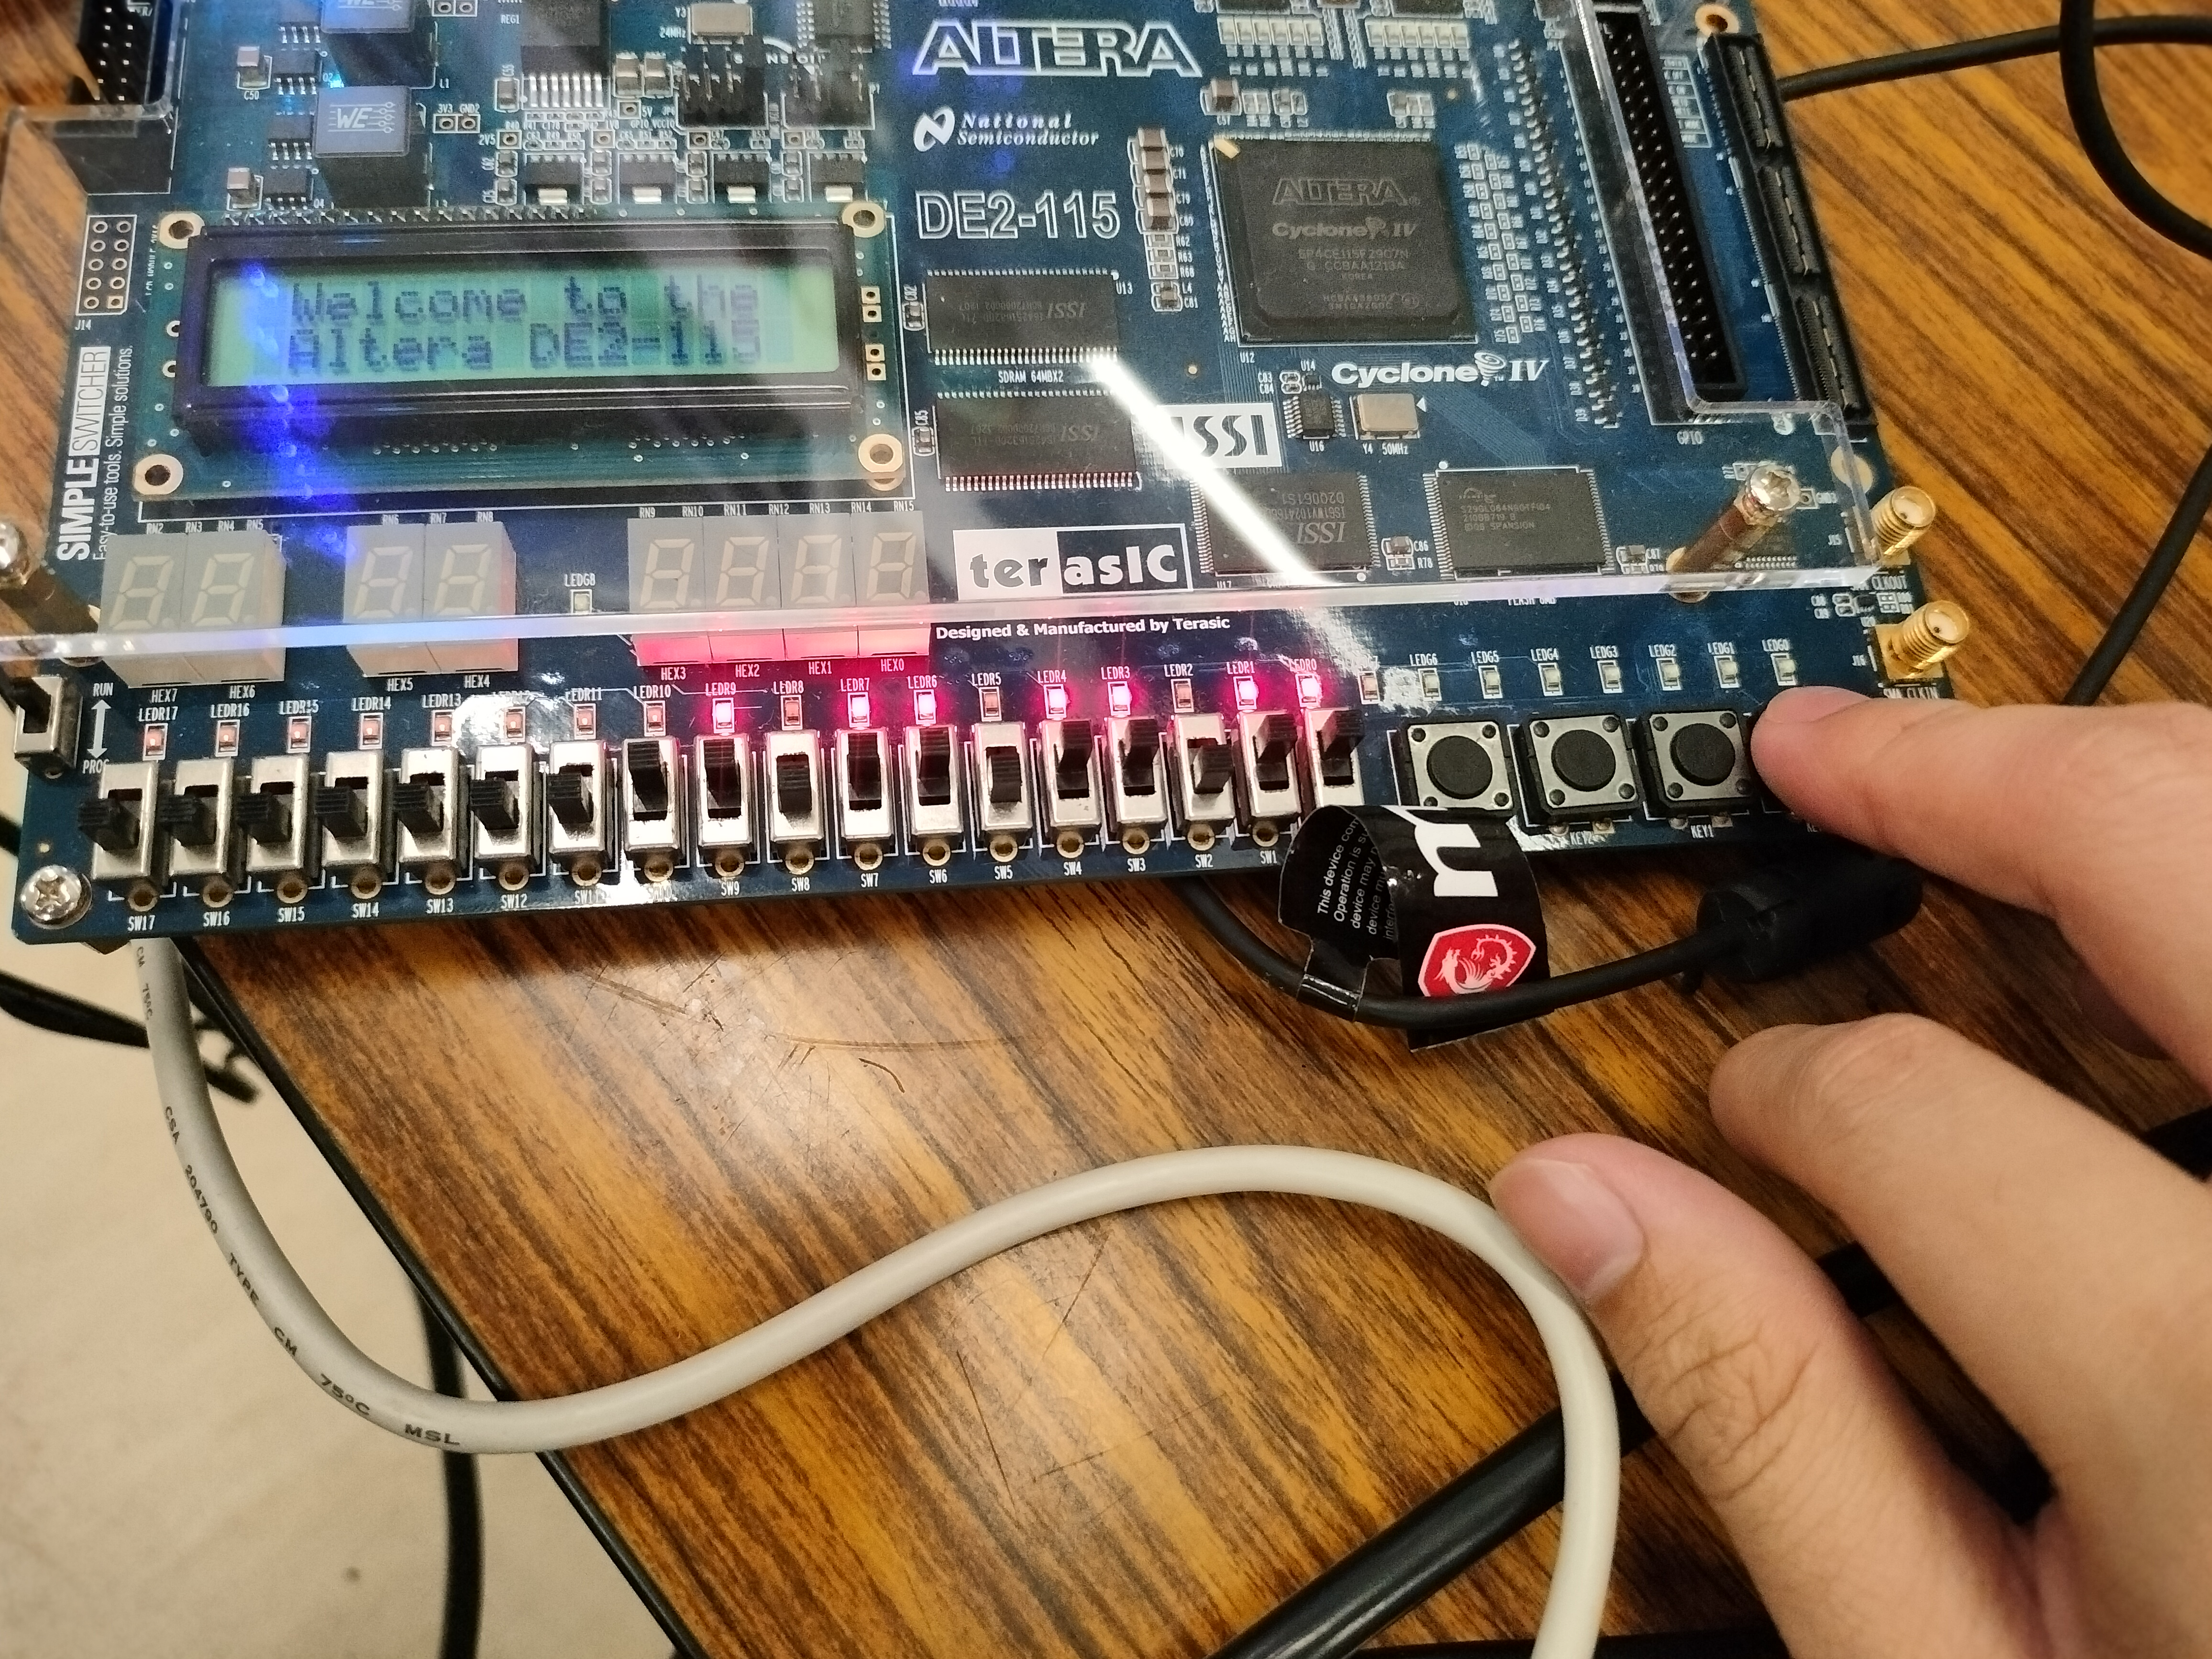
\includegraphics[width=0.5\textwidth]{./Photo/IMG20260513212848.jpg} \\
\bottomrule
\end{longtable}

\subsubsection{2. 平行載入 (Parallel Load)}
\begin{longtable}{p{5cm} c}
\toprule
狀態描述 & 實體照片 \\
\midrule
\textbf{設定輸入值}：調整 SW9~SW0 準備載入特定位元模式。 & 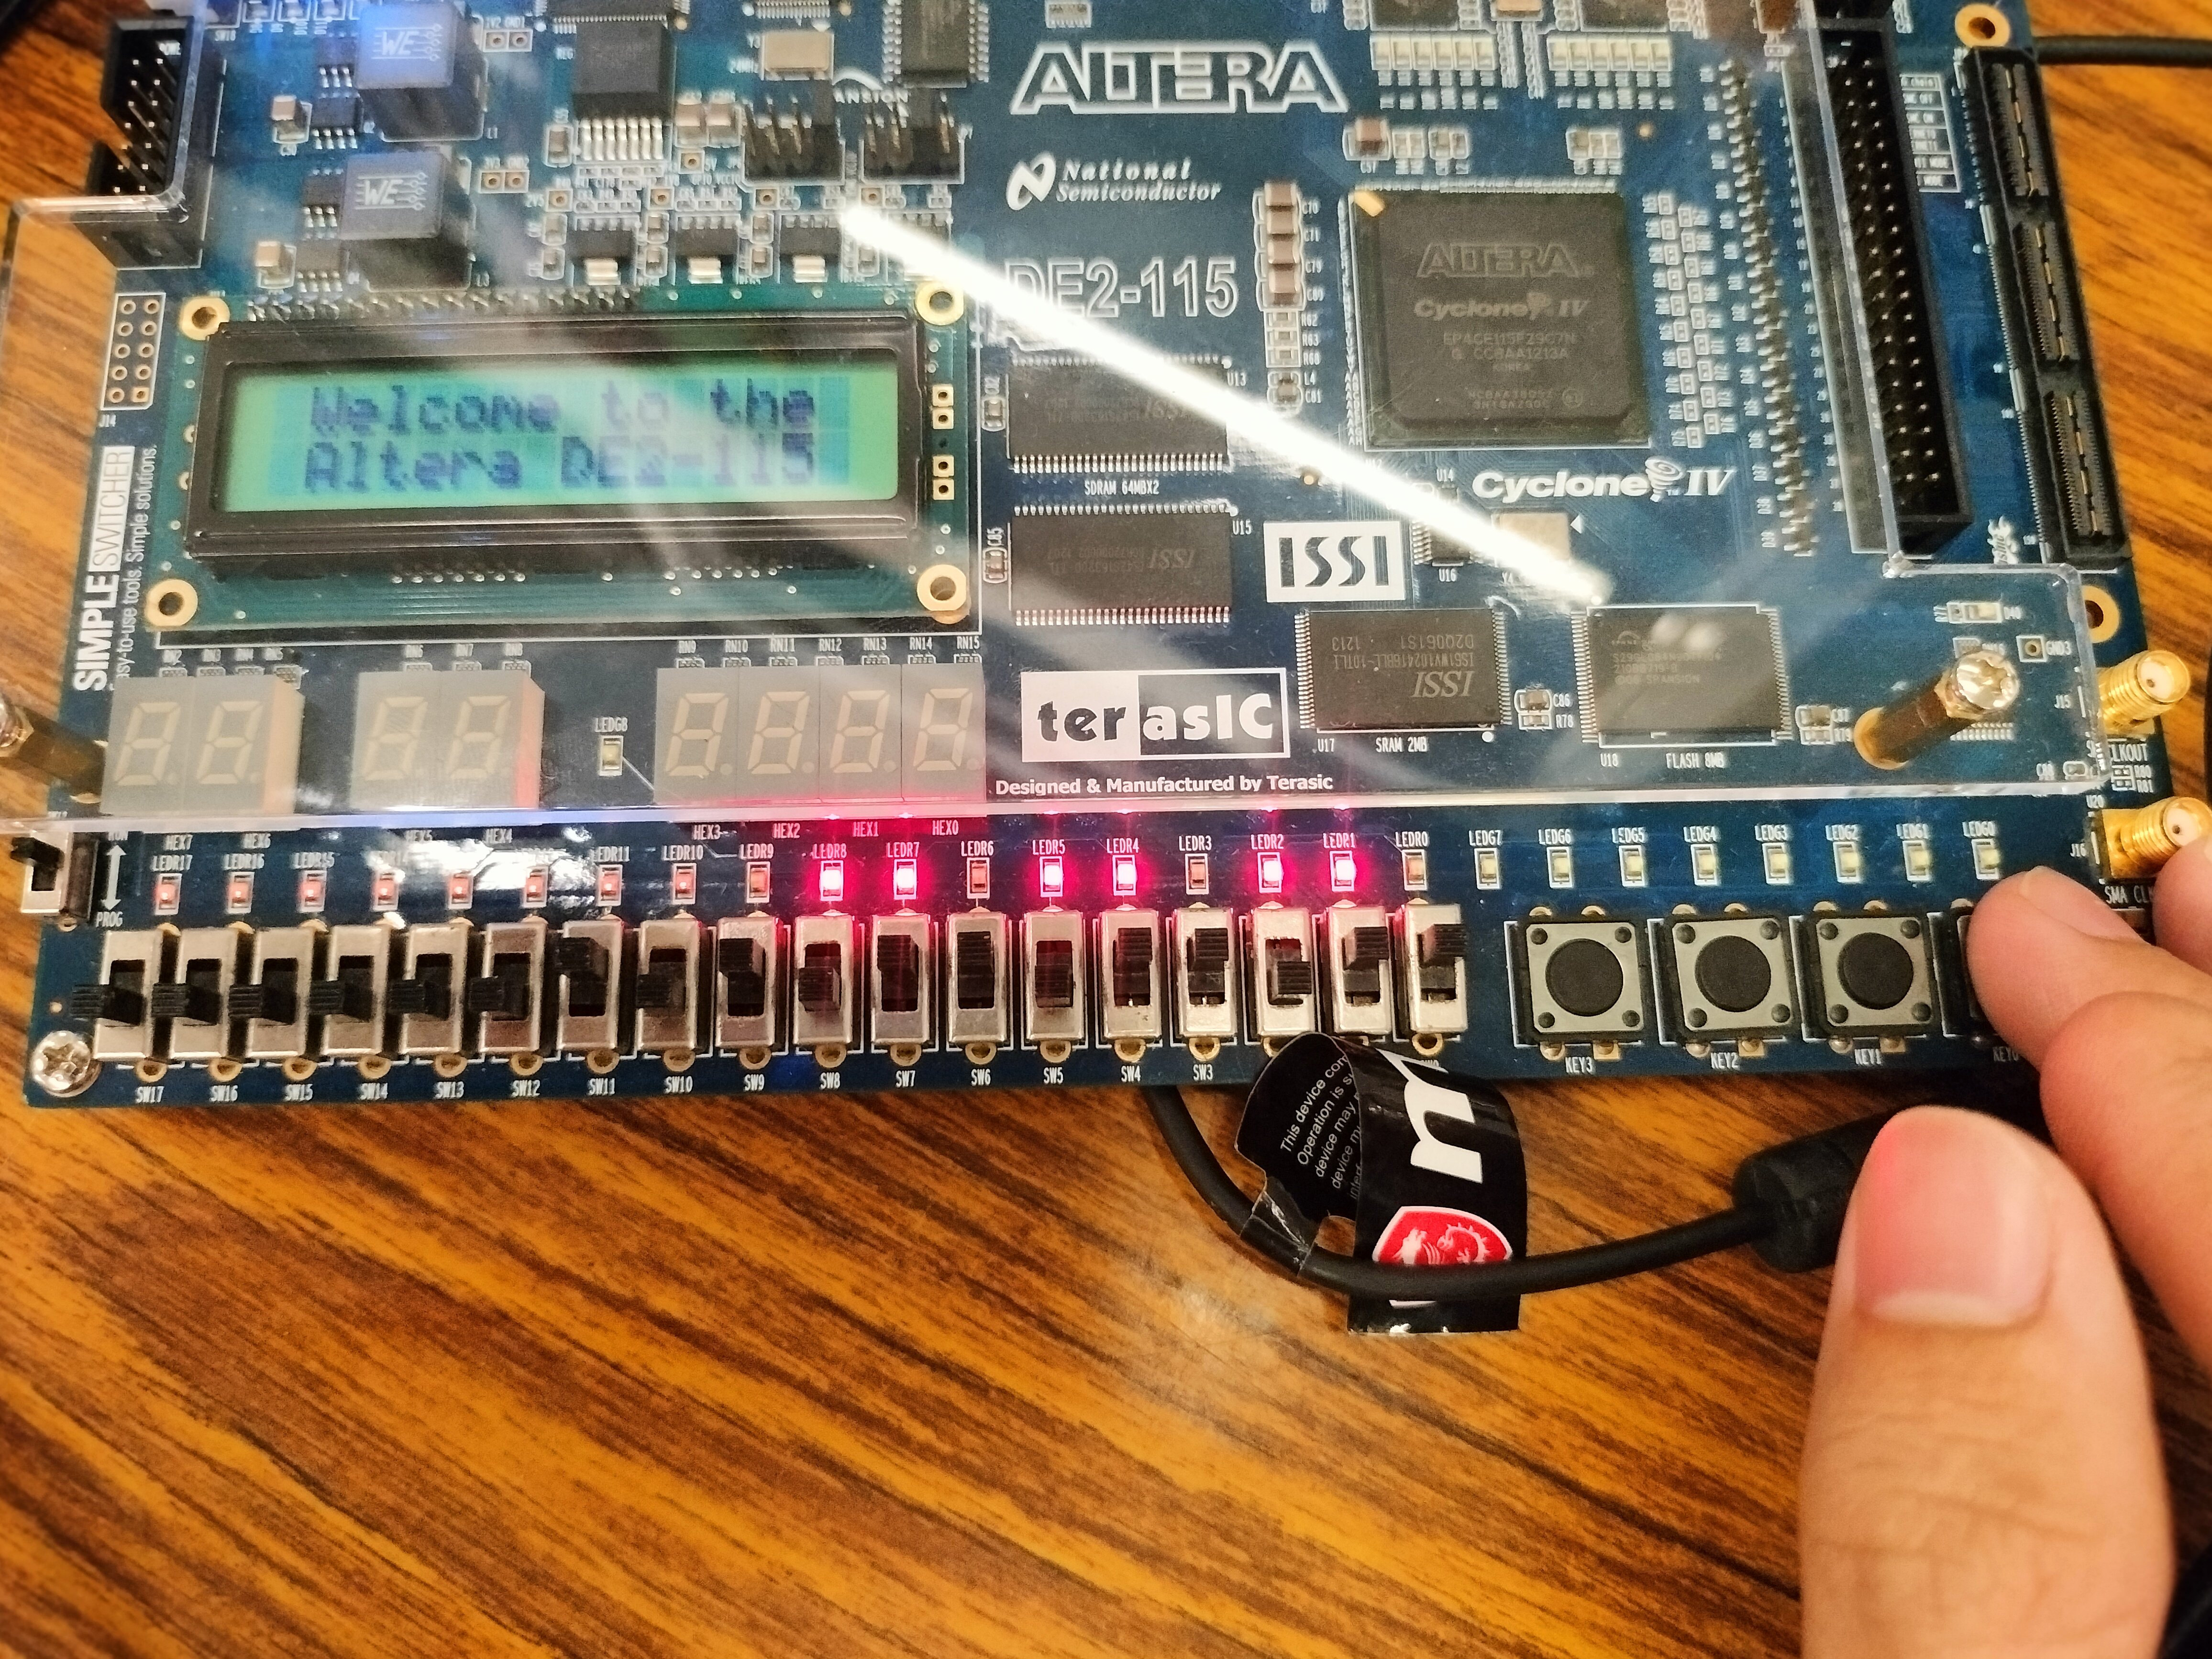
\includegraphics[width=0.5\textwidth]{./Photo/IMG20260513213334.jpg} \\
\textbf{載入範例 1}：成功載入模式（如中間位元亮起）。 & 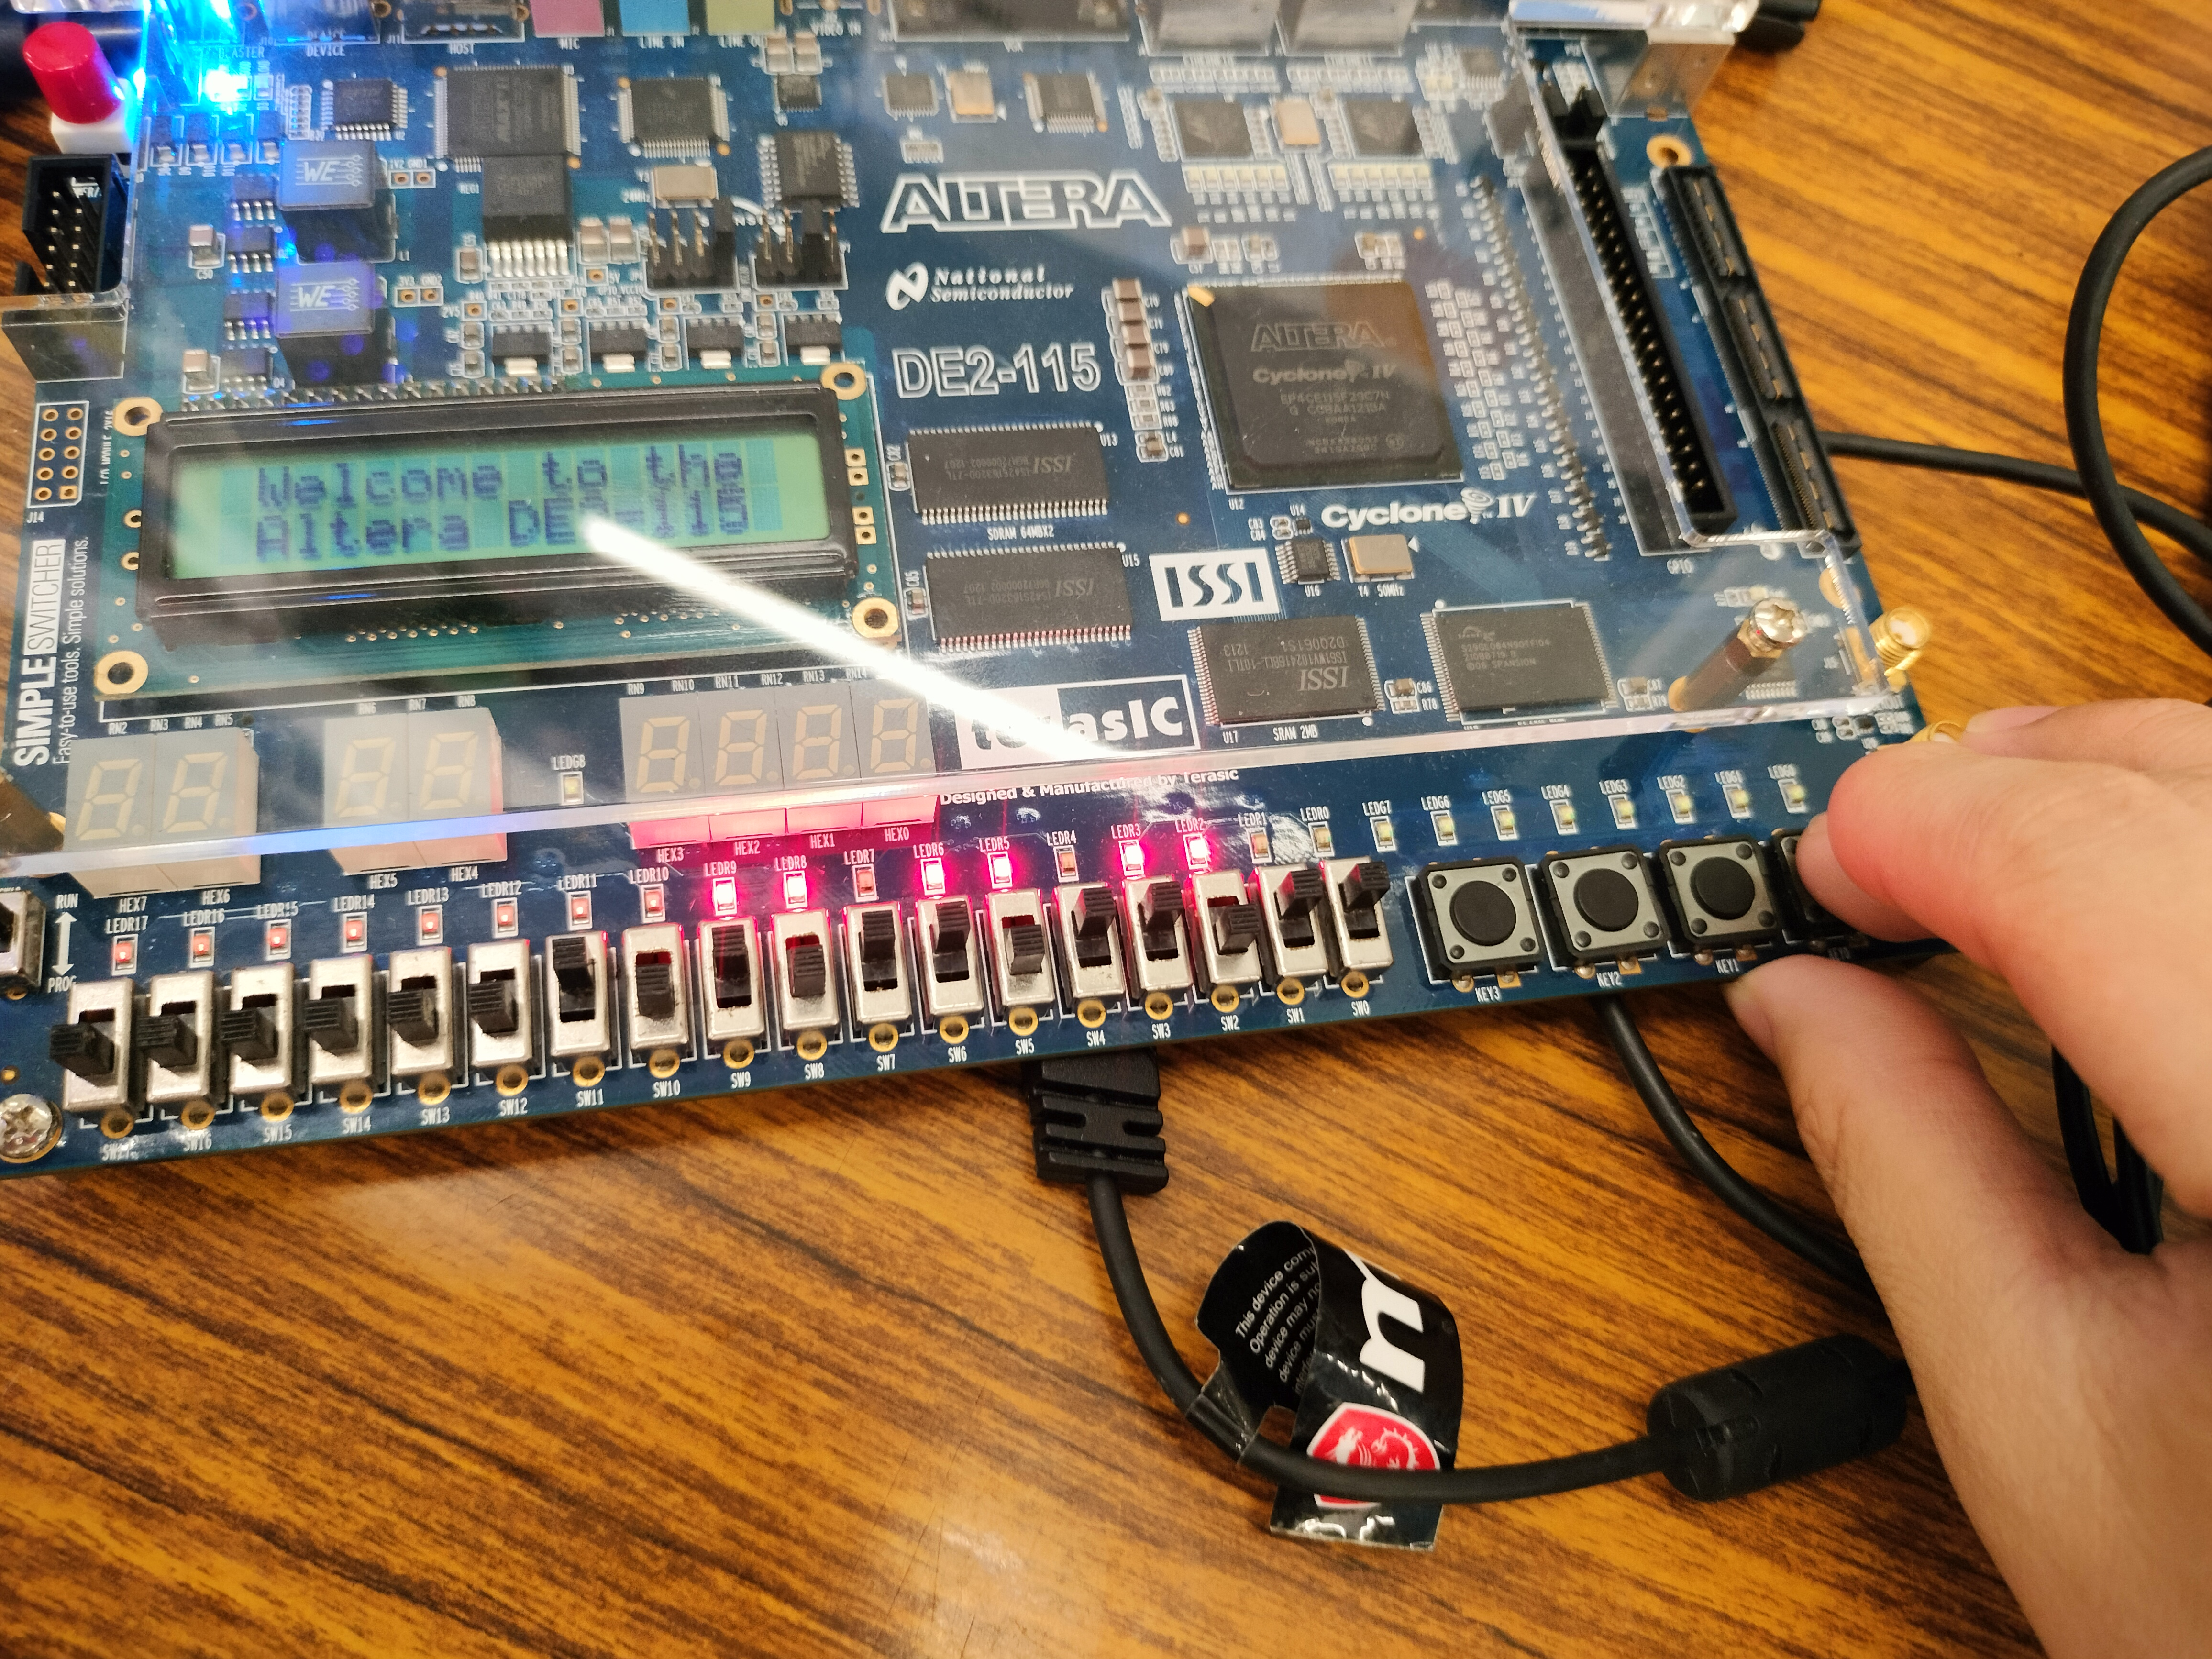
\includegraphics[width=0.5\textwidth]{./Photo/IMG20260513213403.jpg} \\
\textbf{載入範例 2}：載入另一種開關組合。 & 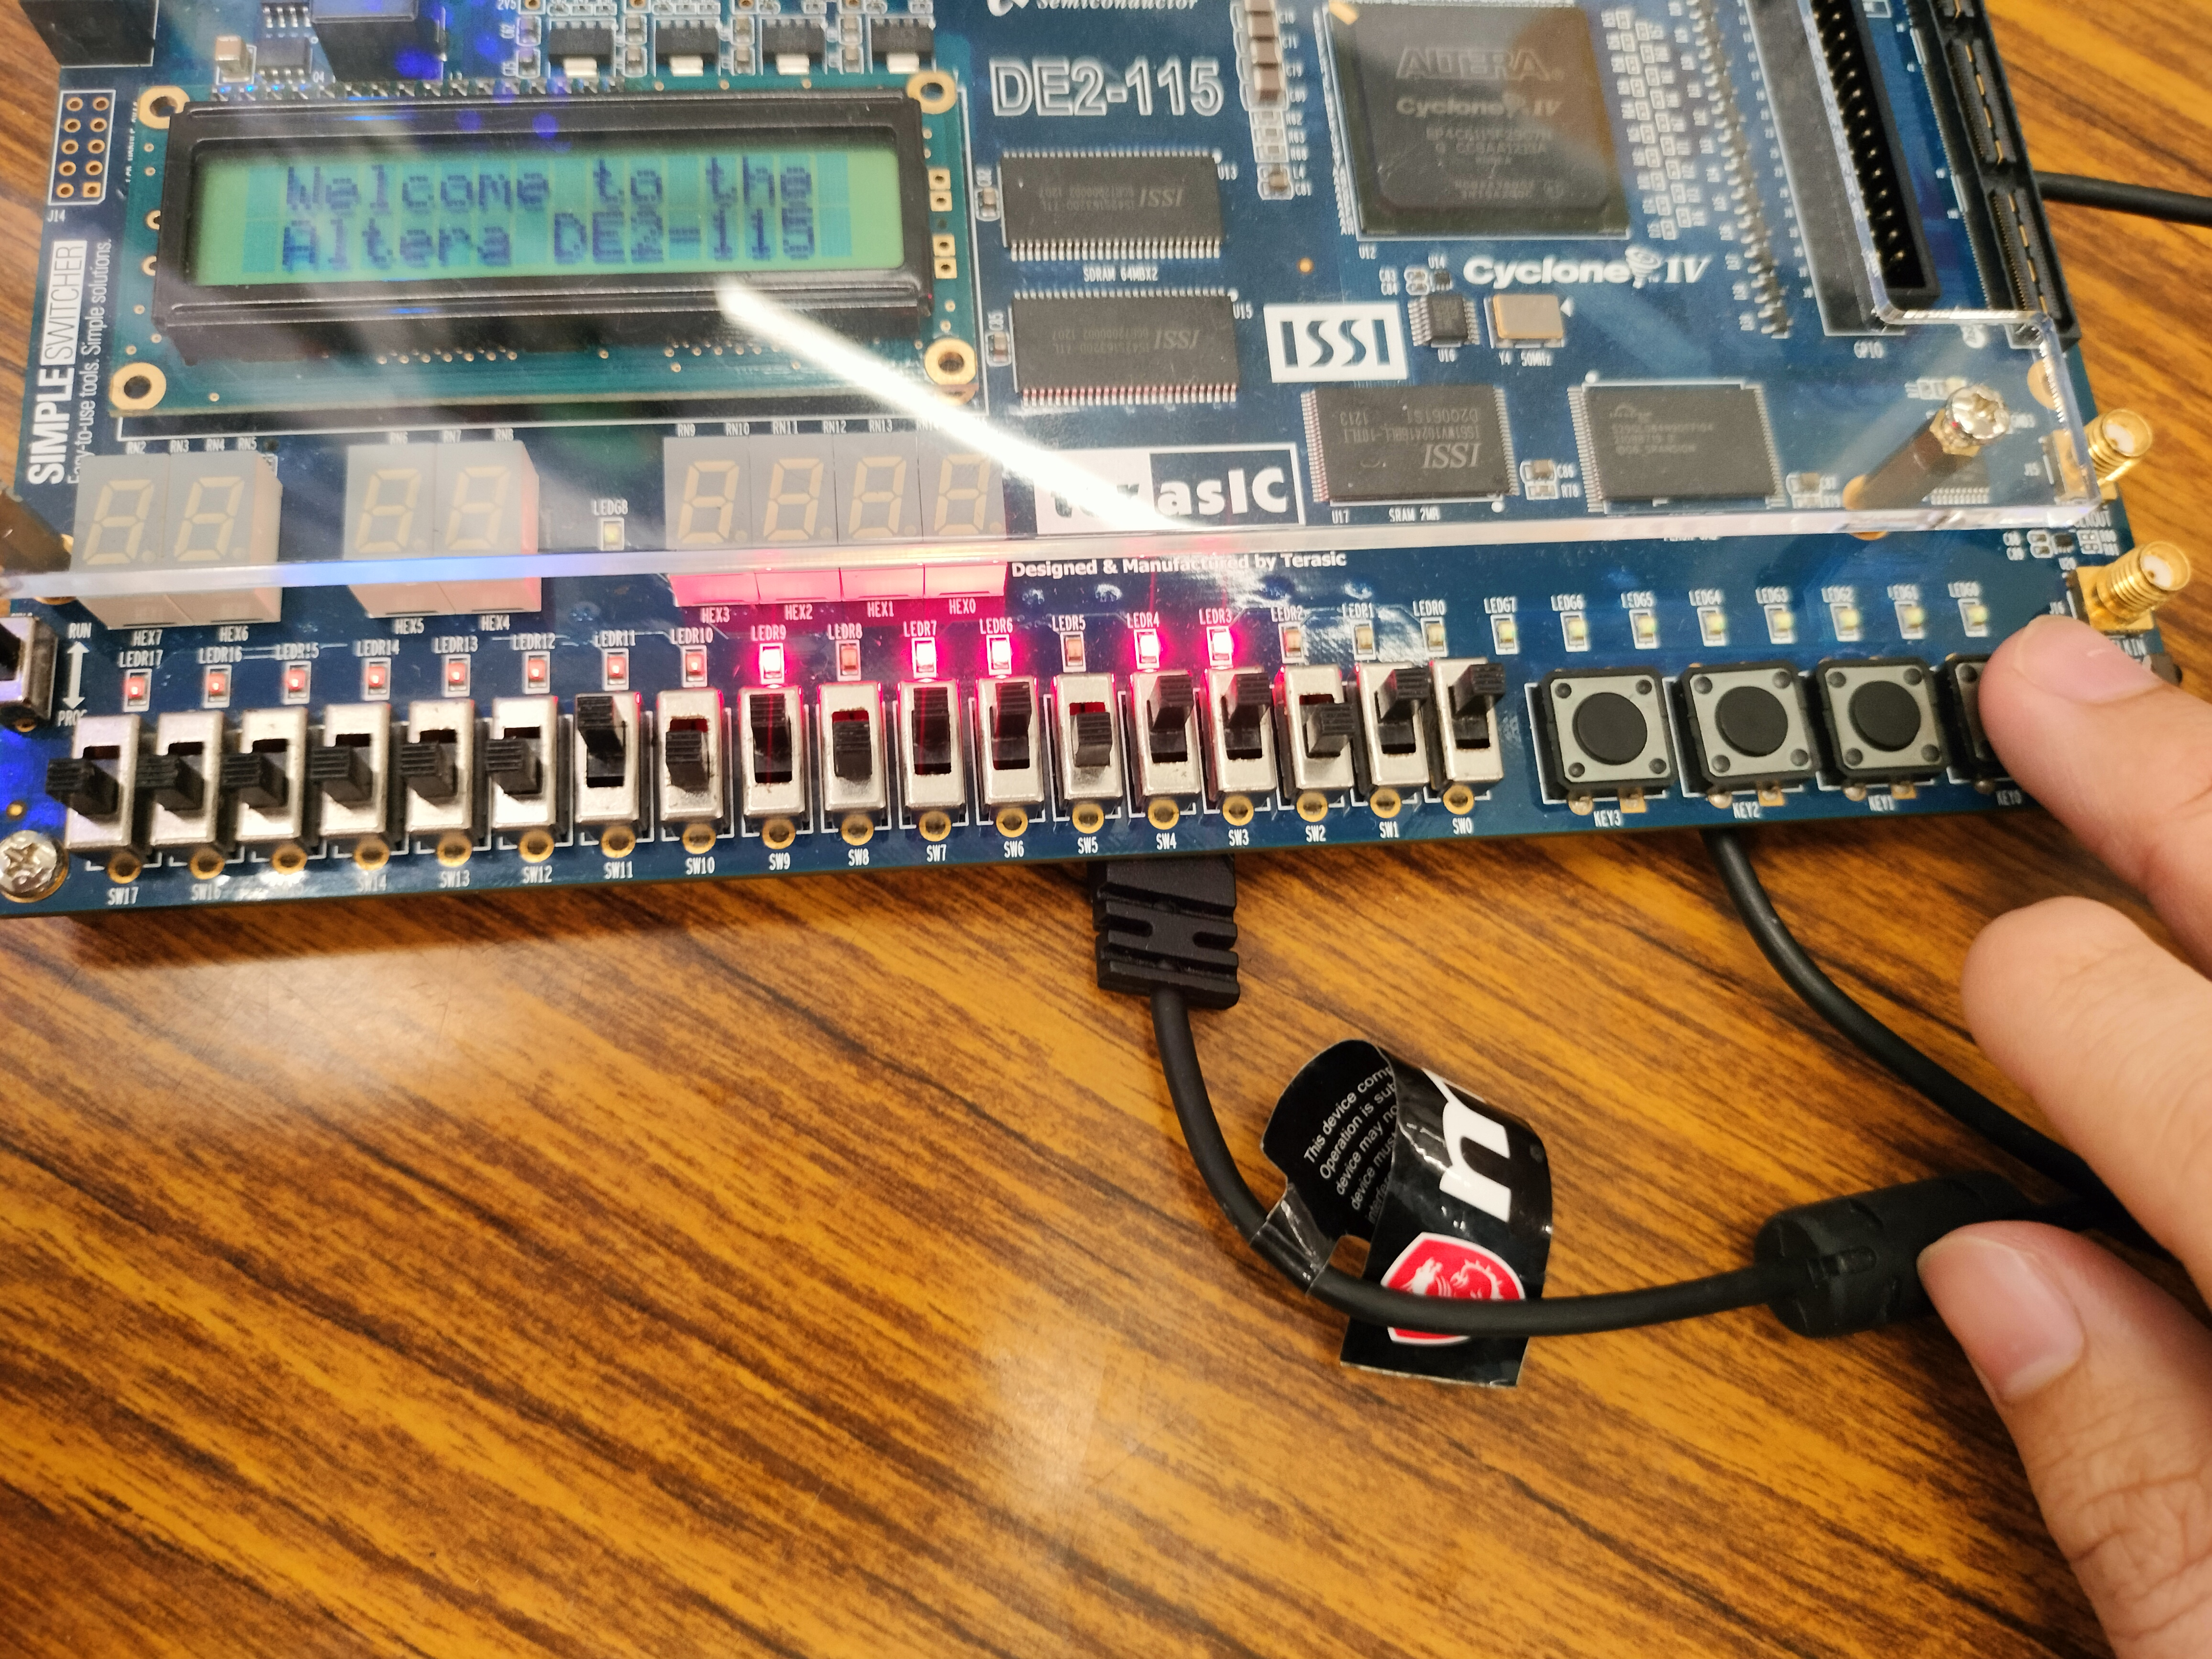
\includegraphics[width=0.5\textwidth]{./Photo/IMG20260513213427.jpg} \\
\textbf{載入範例 3}：更改開關後再次載入不同模式。 & 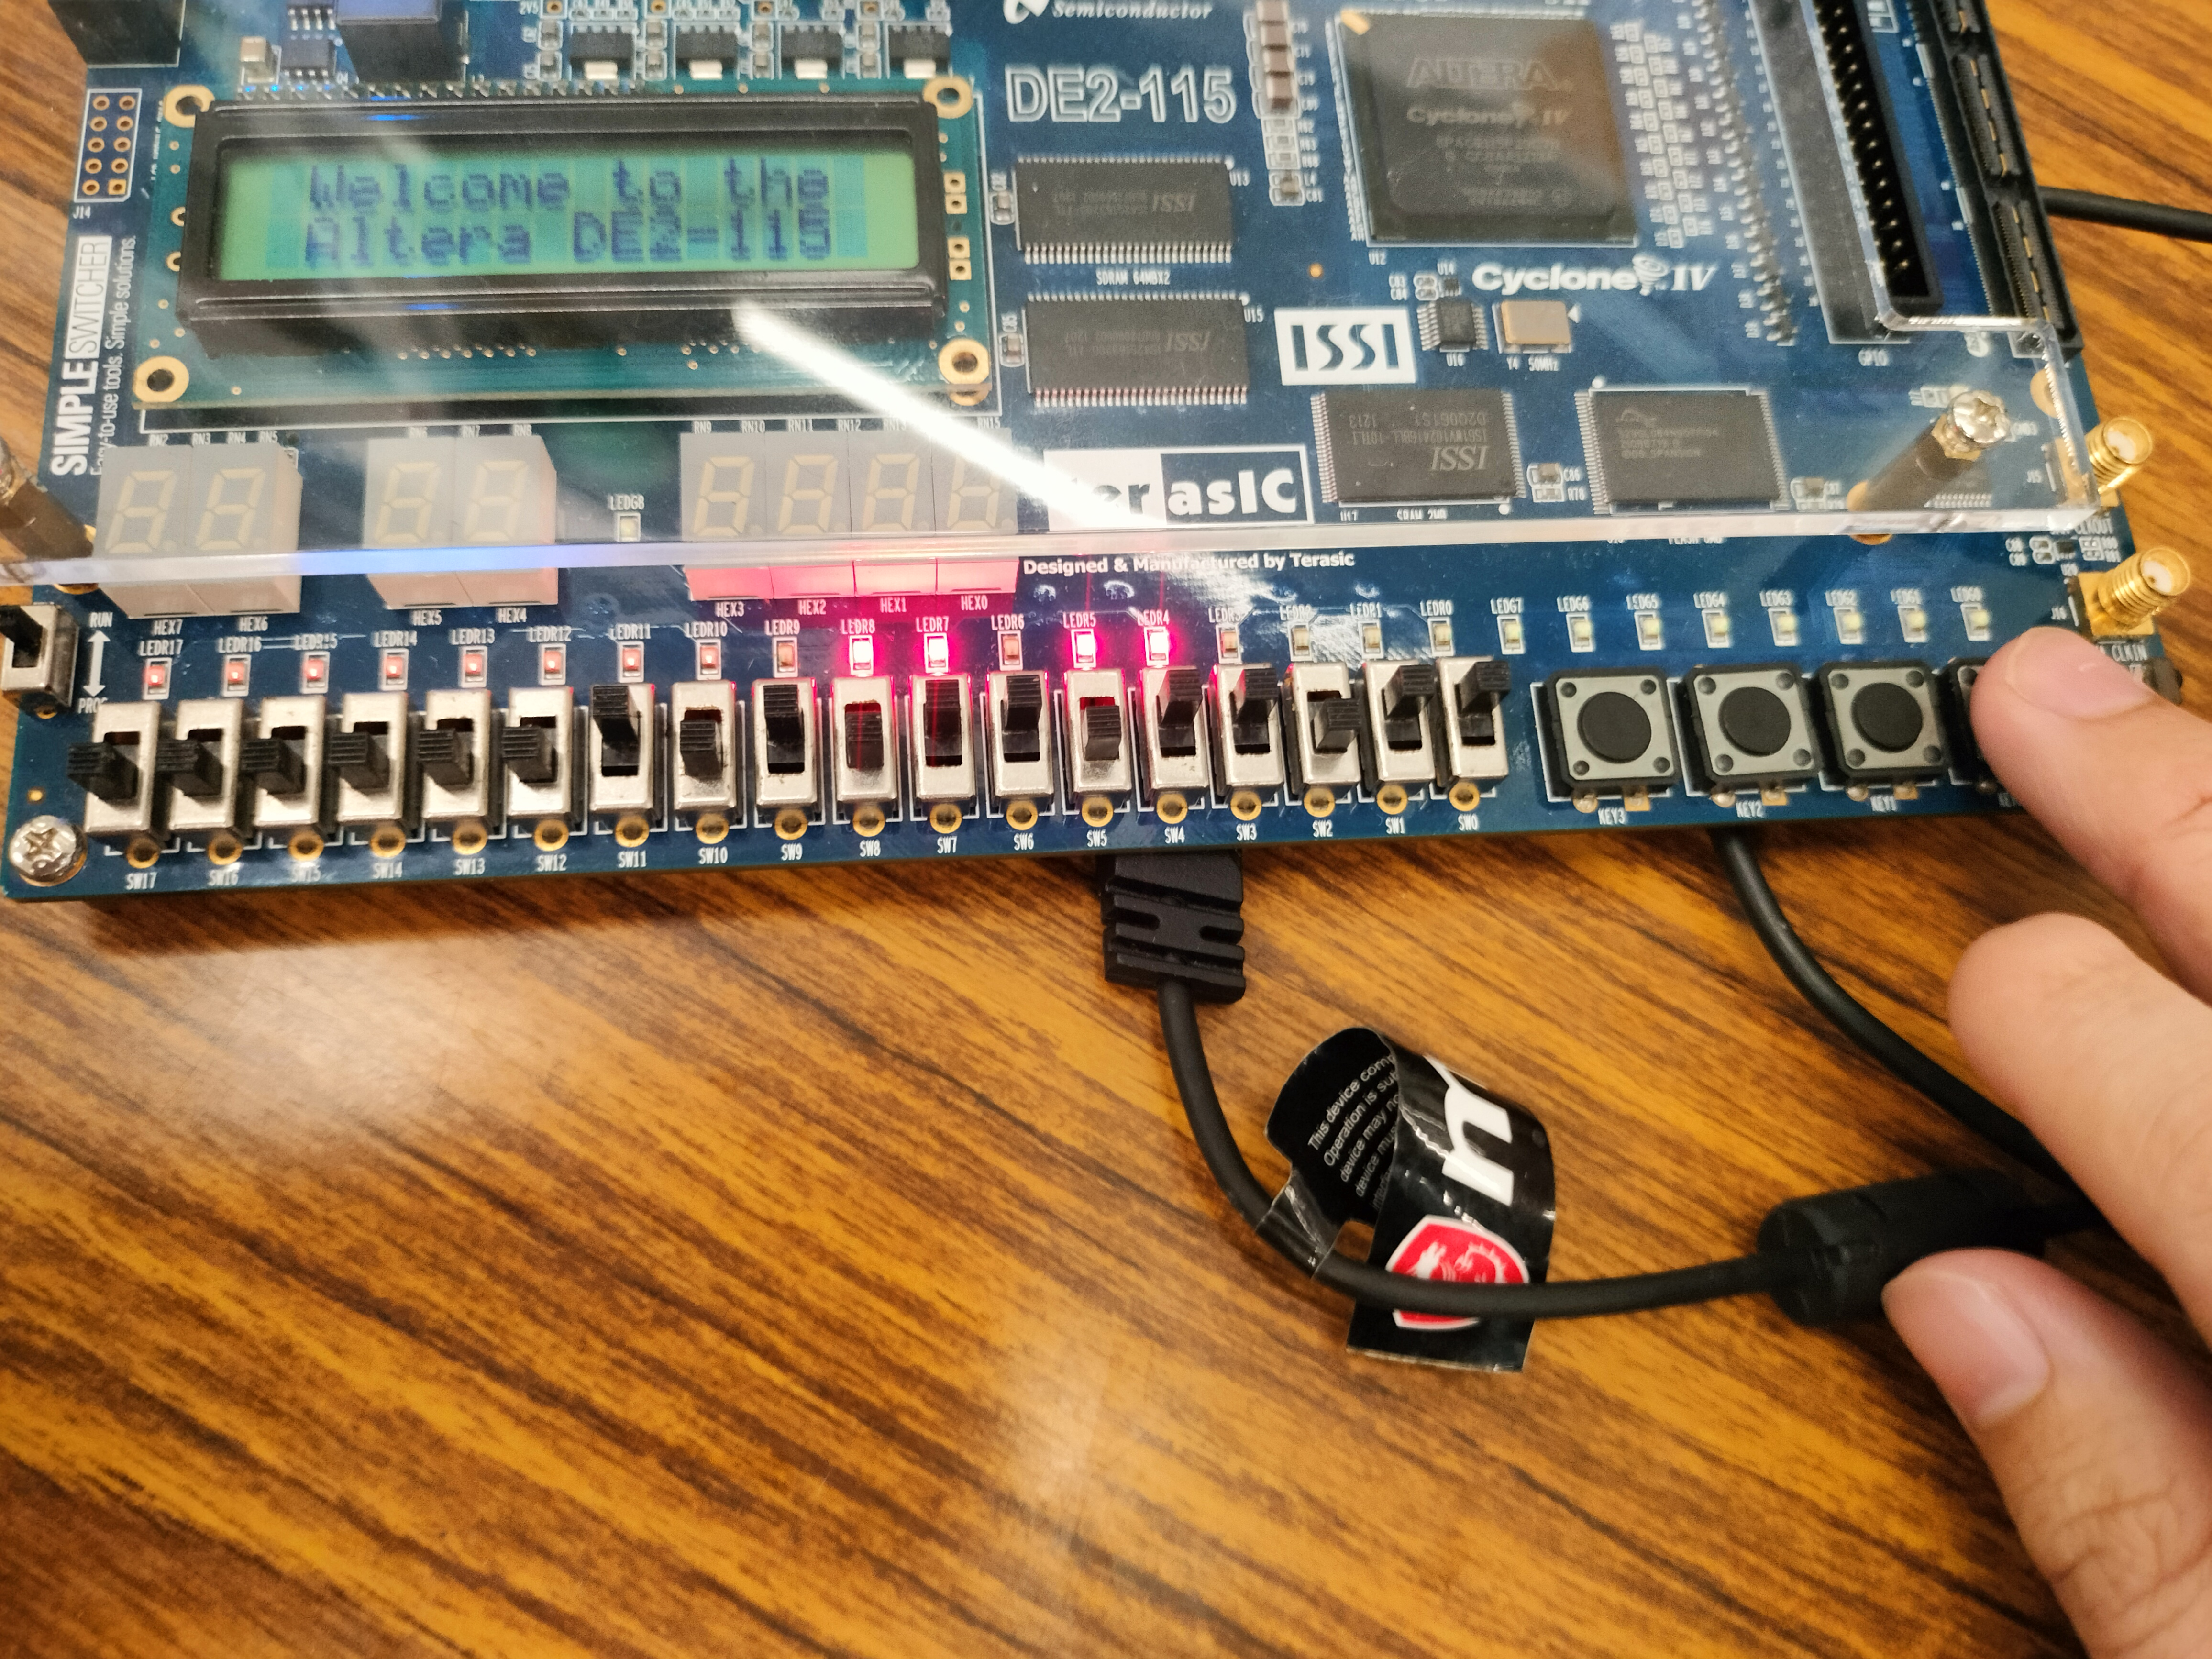
\includegraphics[width=0.5\textwidth]{./Photo/IMG20260513213435.jpg} \\
\textbf{載入範例 4}：測試全亮或特定模式。 & 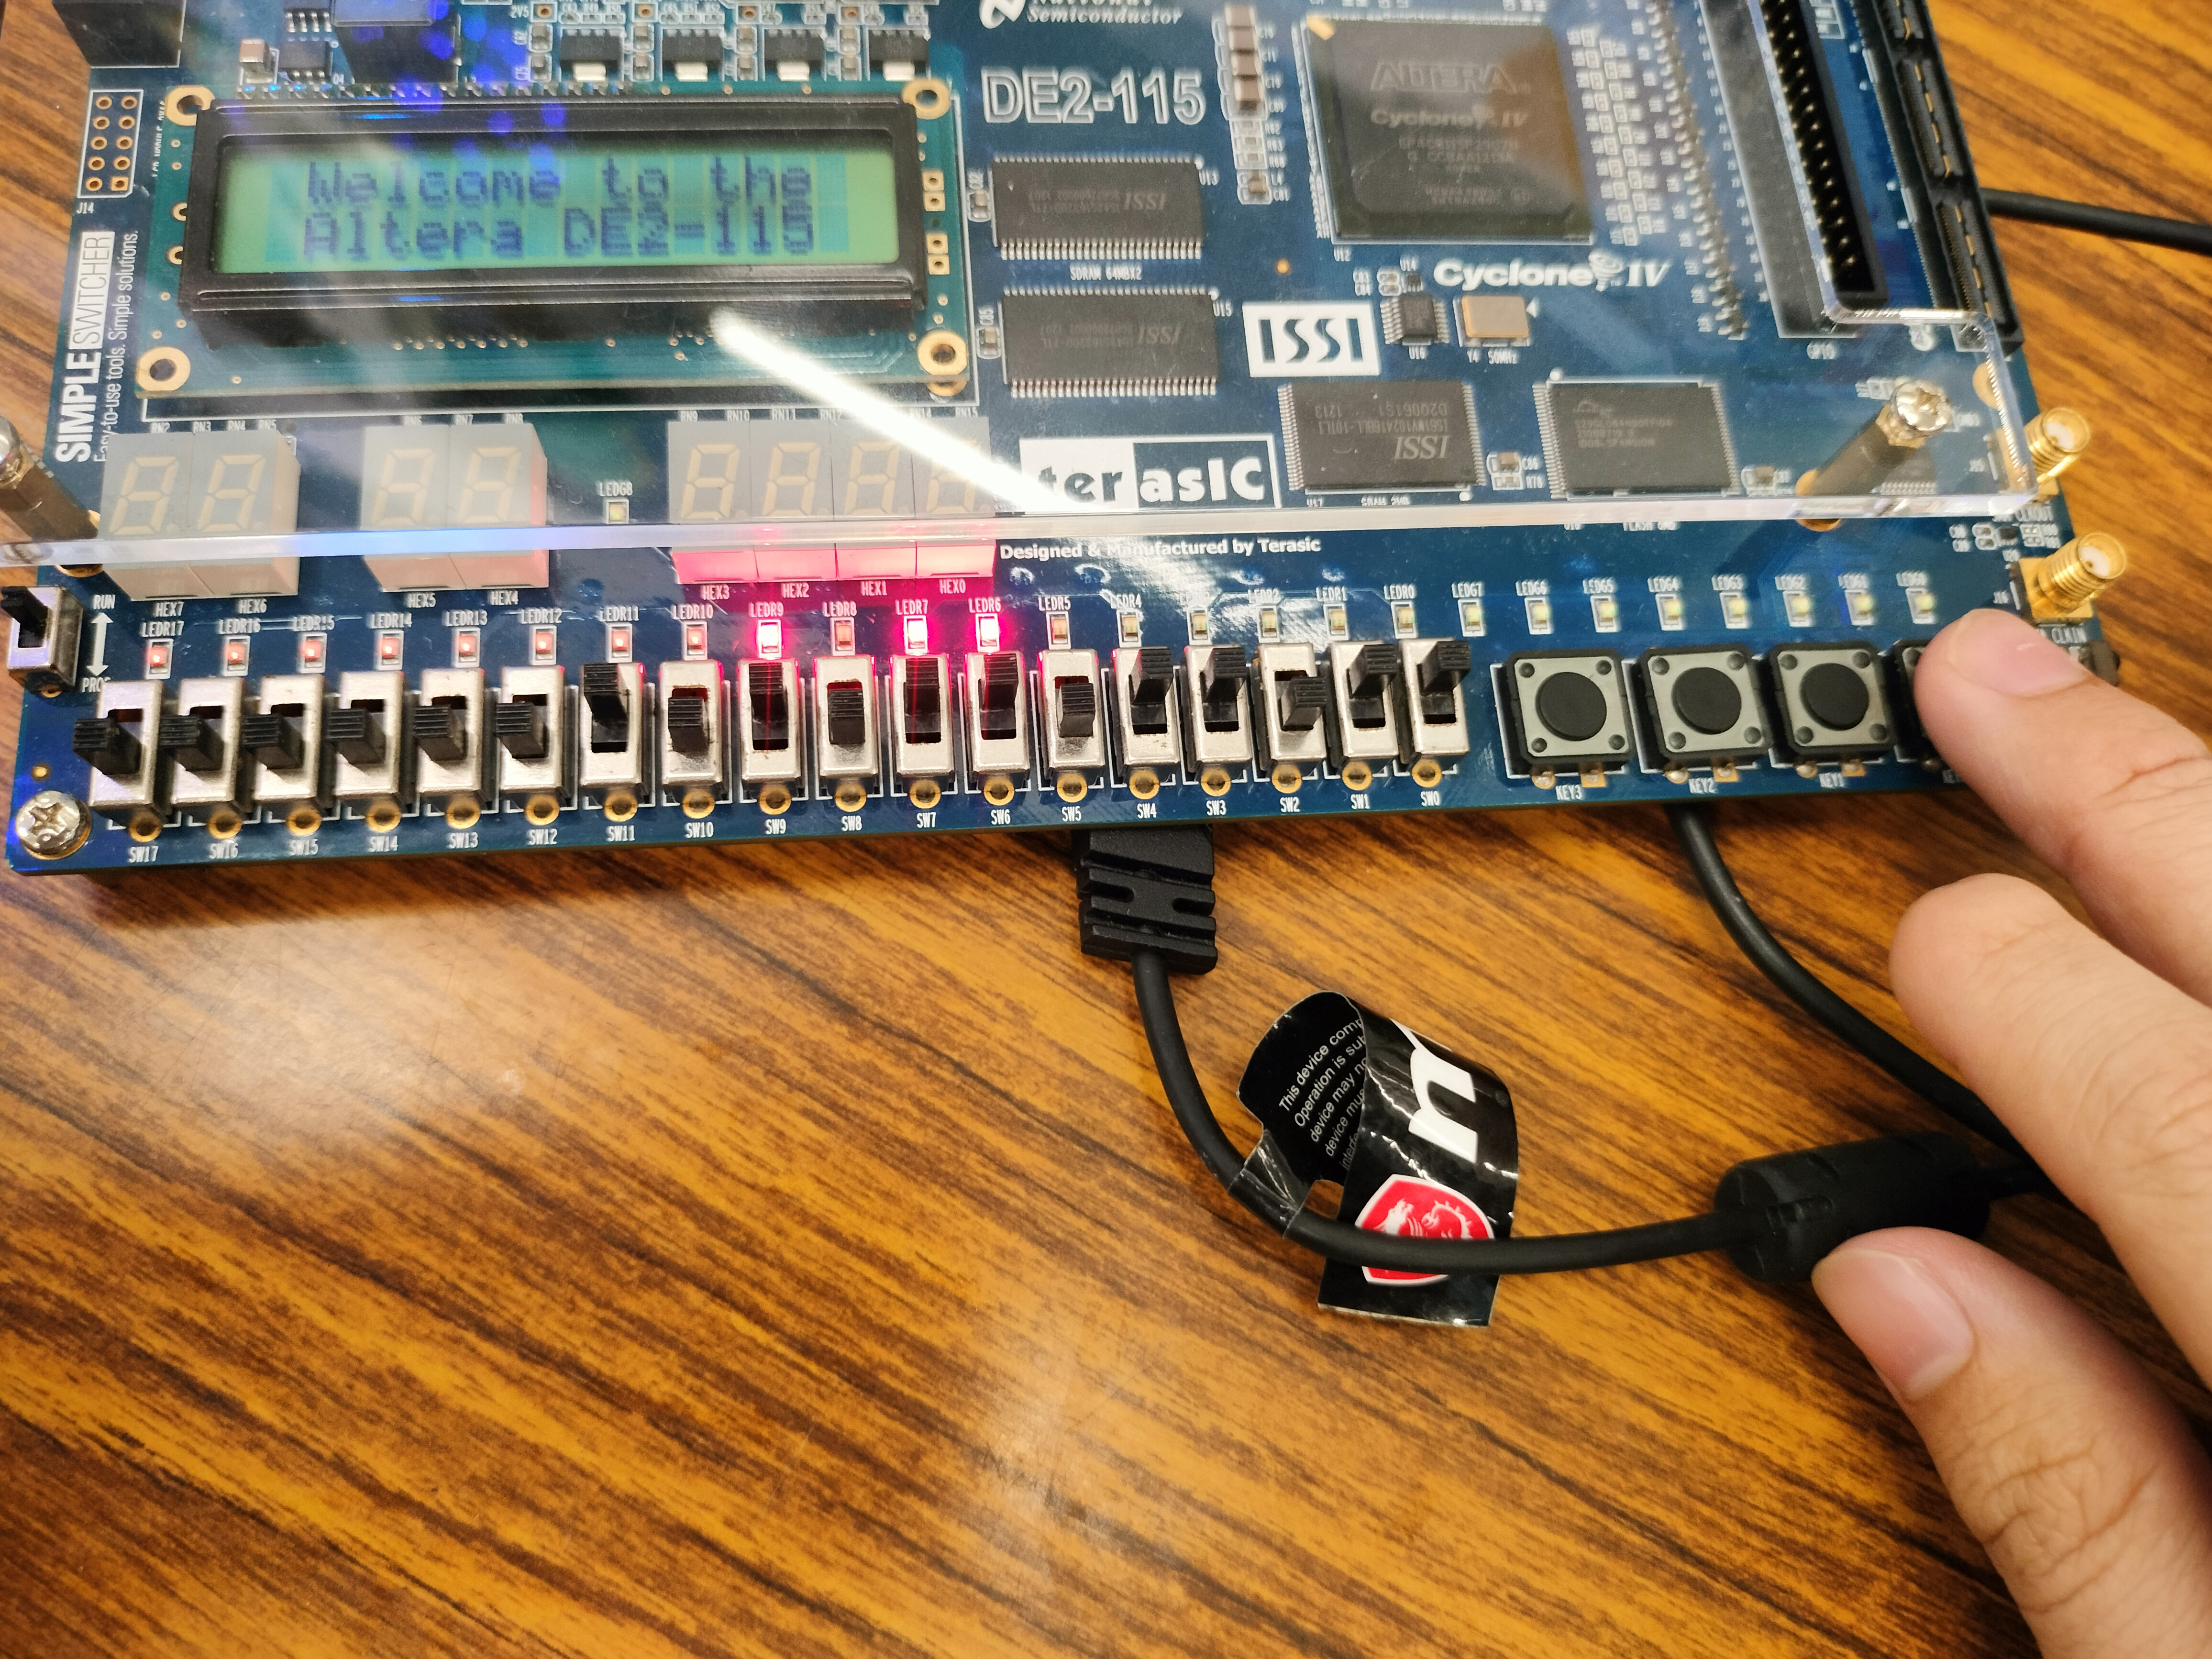
\includegraphics[width=0.5\textwidth]{./Photo/IMG20260513213439.jpg} \\
\bottomrule
\end{longtable}

\subsubsection{3. 左移操作 (Left Shift)}
\begin{longtable}{p{5cm} c}
\toprule
狀態描述 & 實體照片 \\
\midrule
\textbf{左移開始}：初始載入之數值。 & 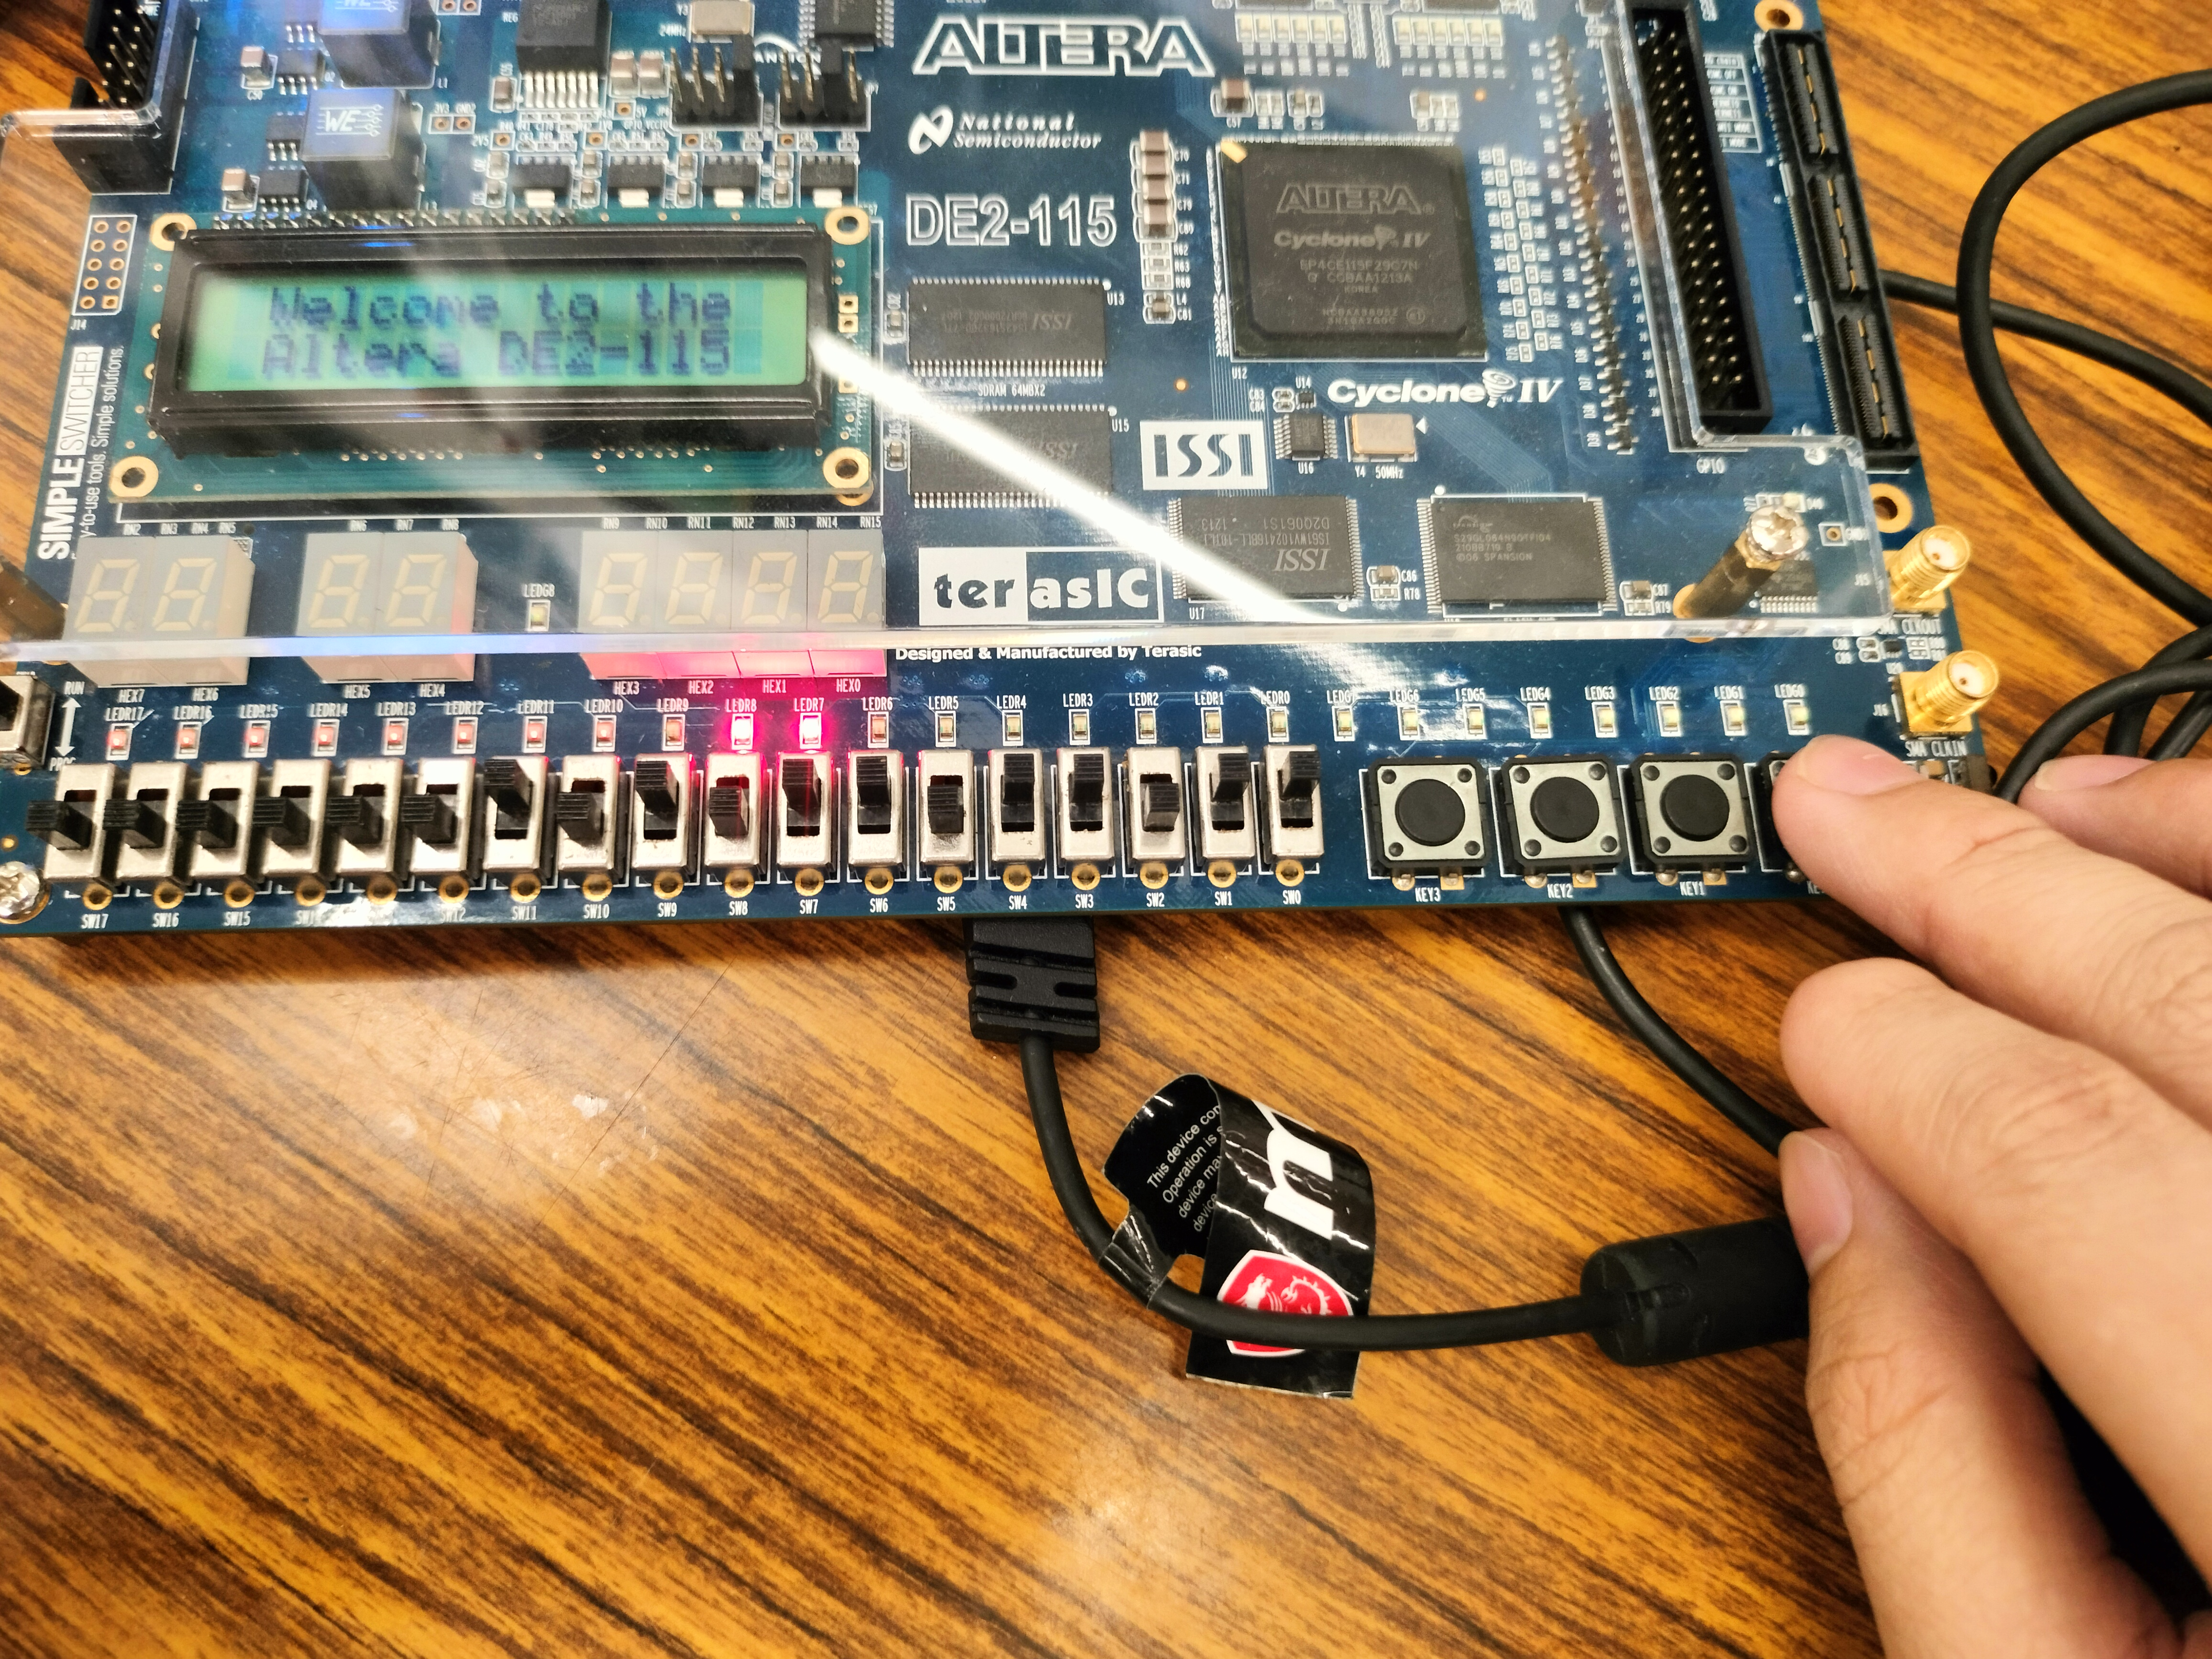
\includegraphics[width=0.5\textwidth]{./Photo/IMG20260513213526.jpg} \\
\textbf{左移過程 1}：按下 KEY0，位元向左（高位元）移動。 & 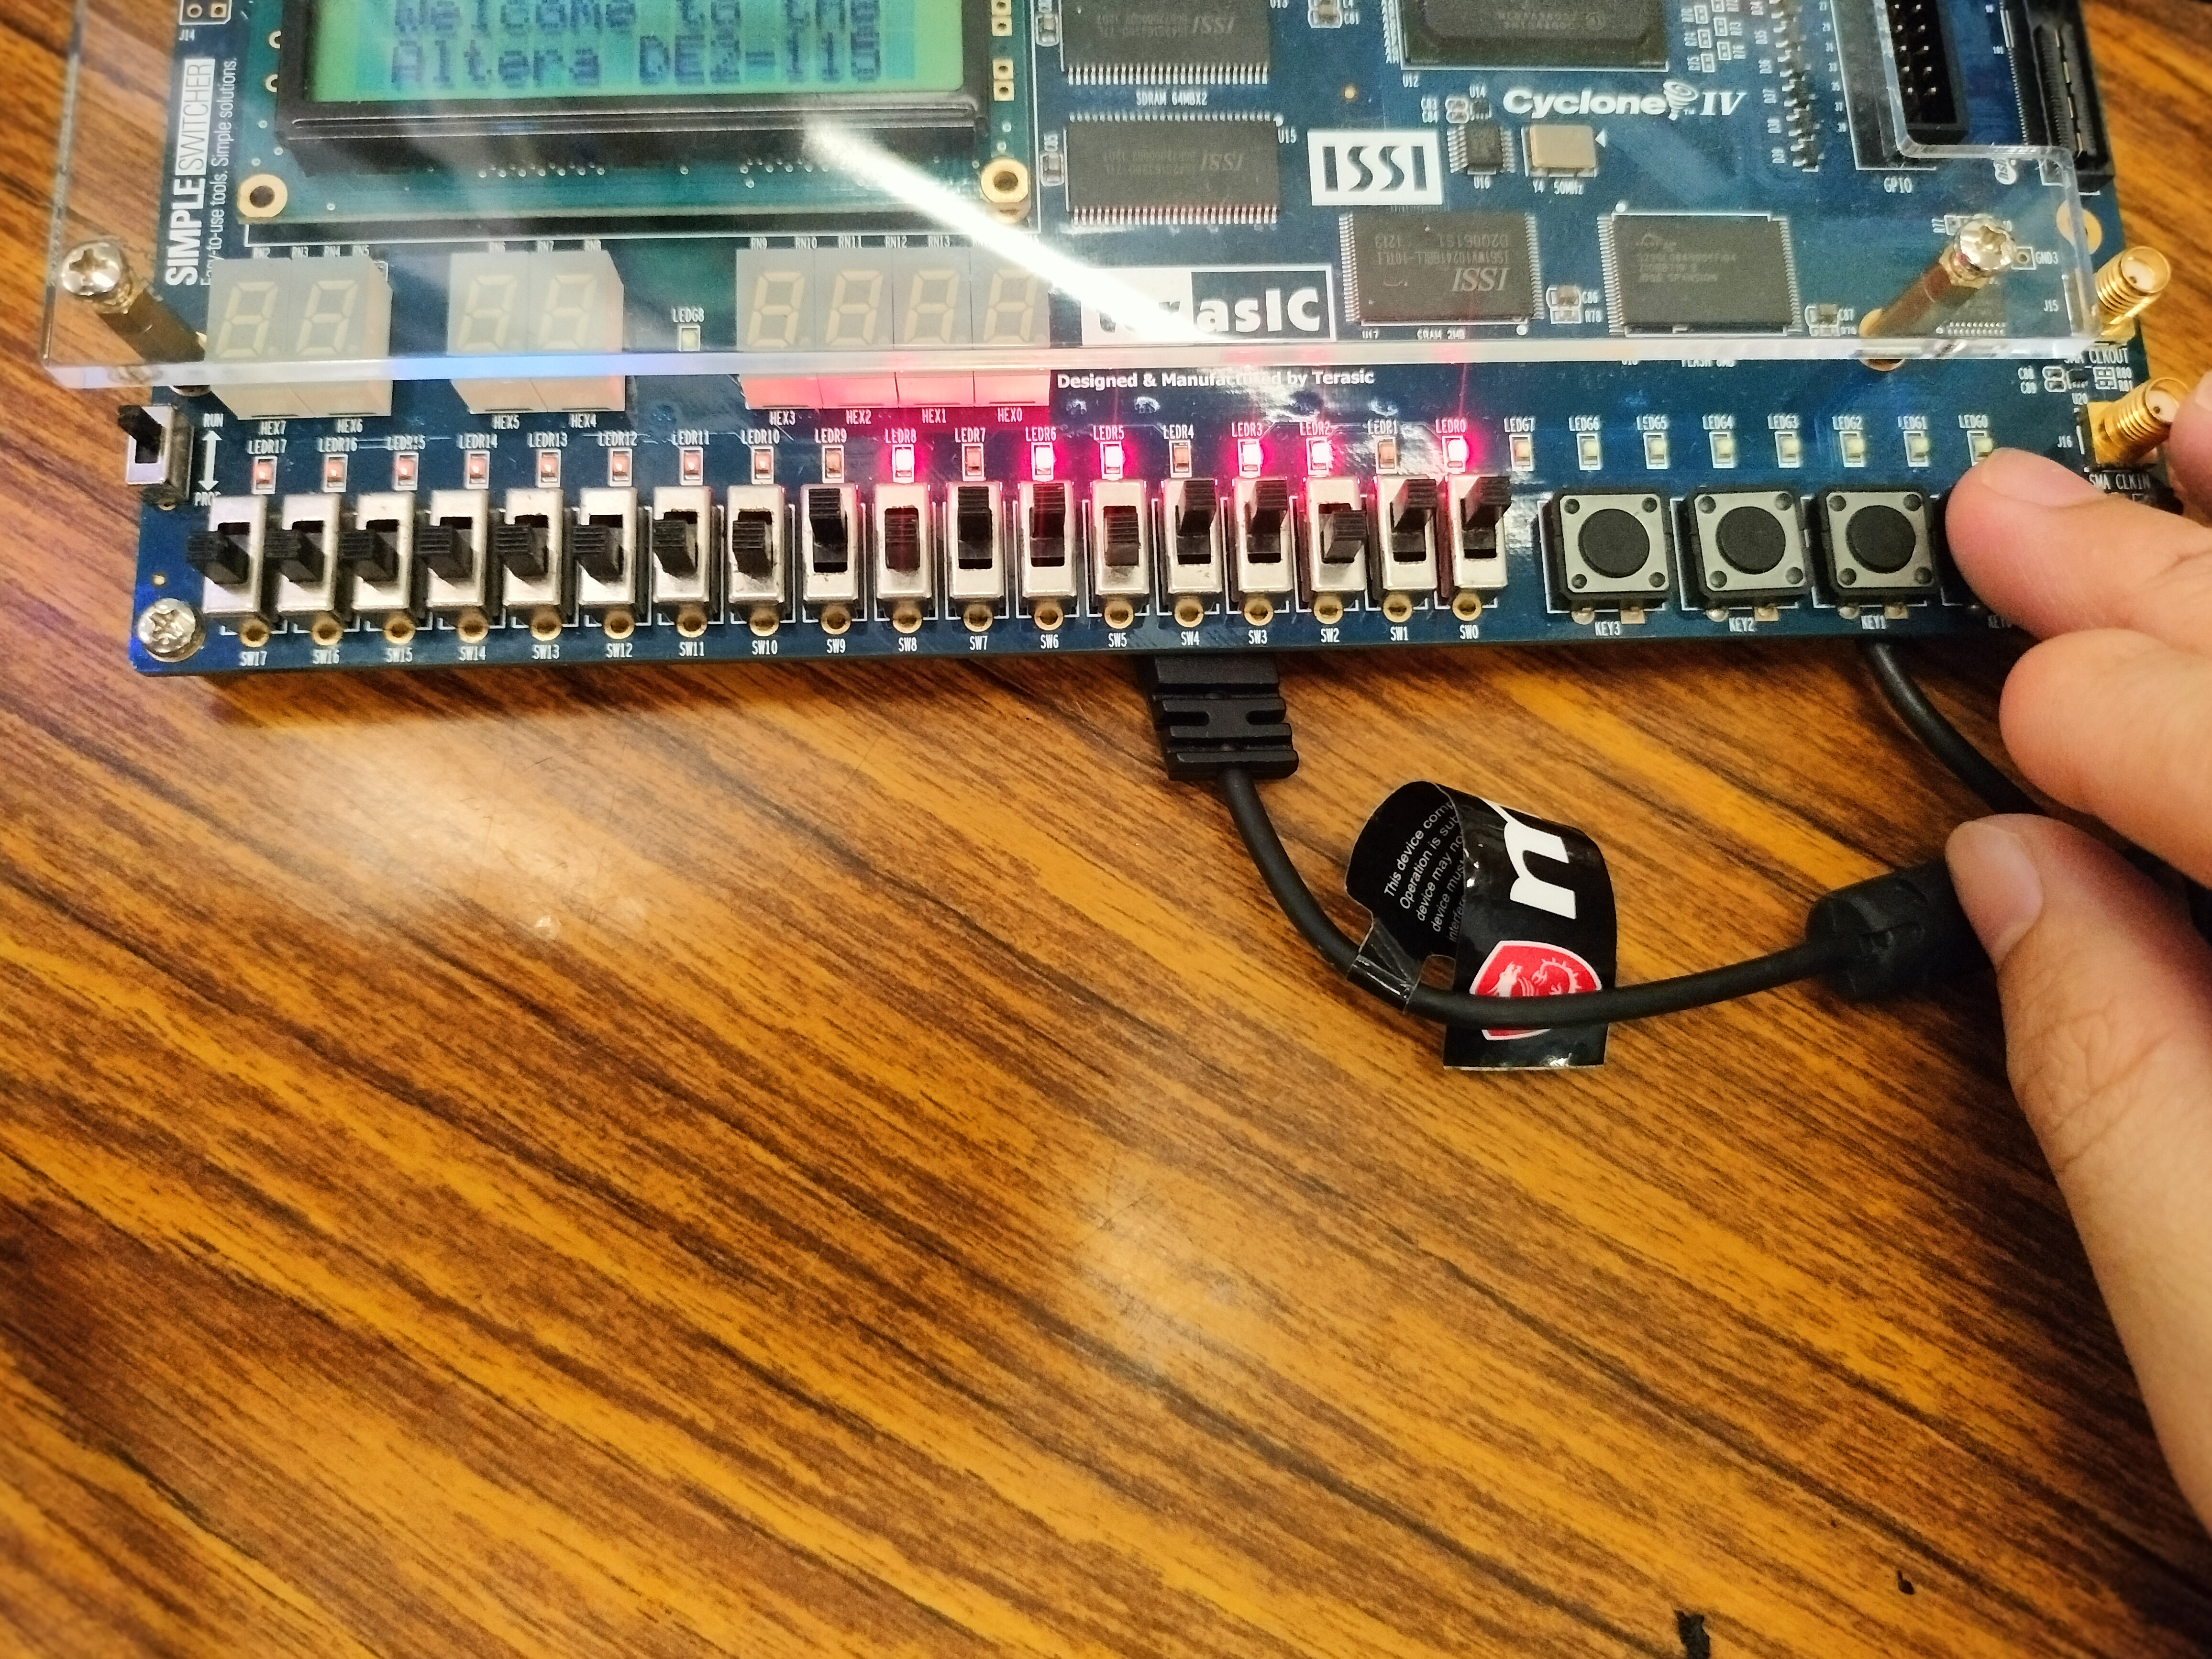
\includegraphics[width=0.5\textwidth]{./Photo/IMG20260513213623.jpg} \\
\textbf{左移過程 2}：連續位移，觀察 LED 往左跳動。 & 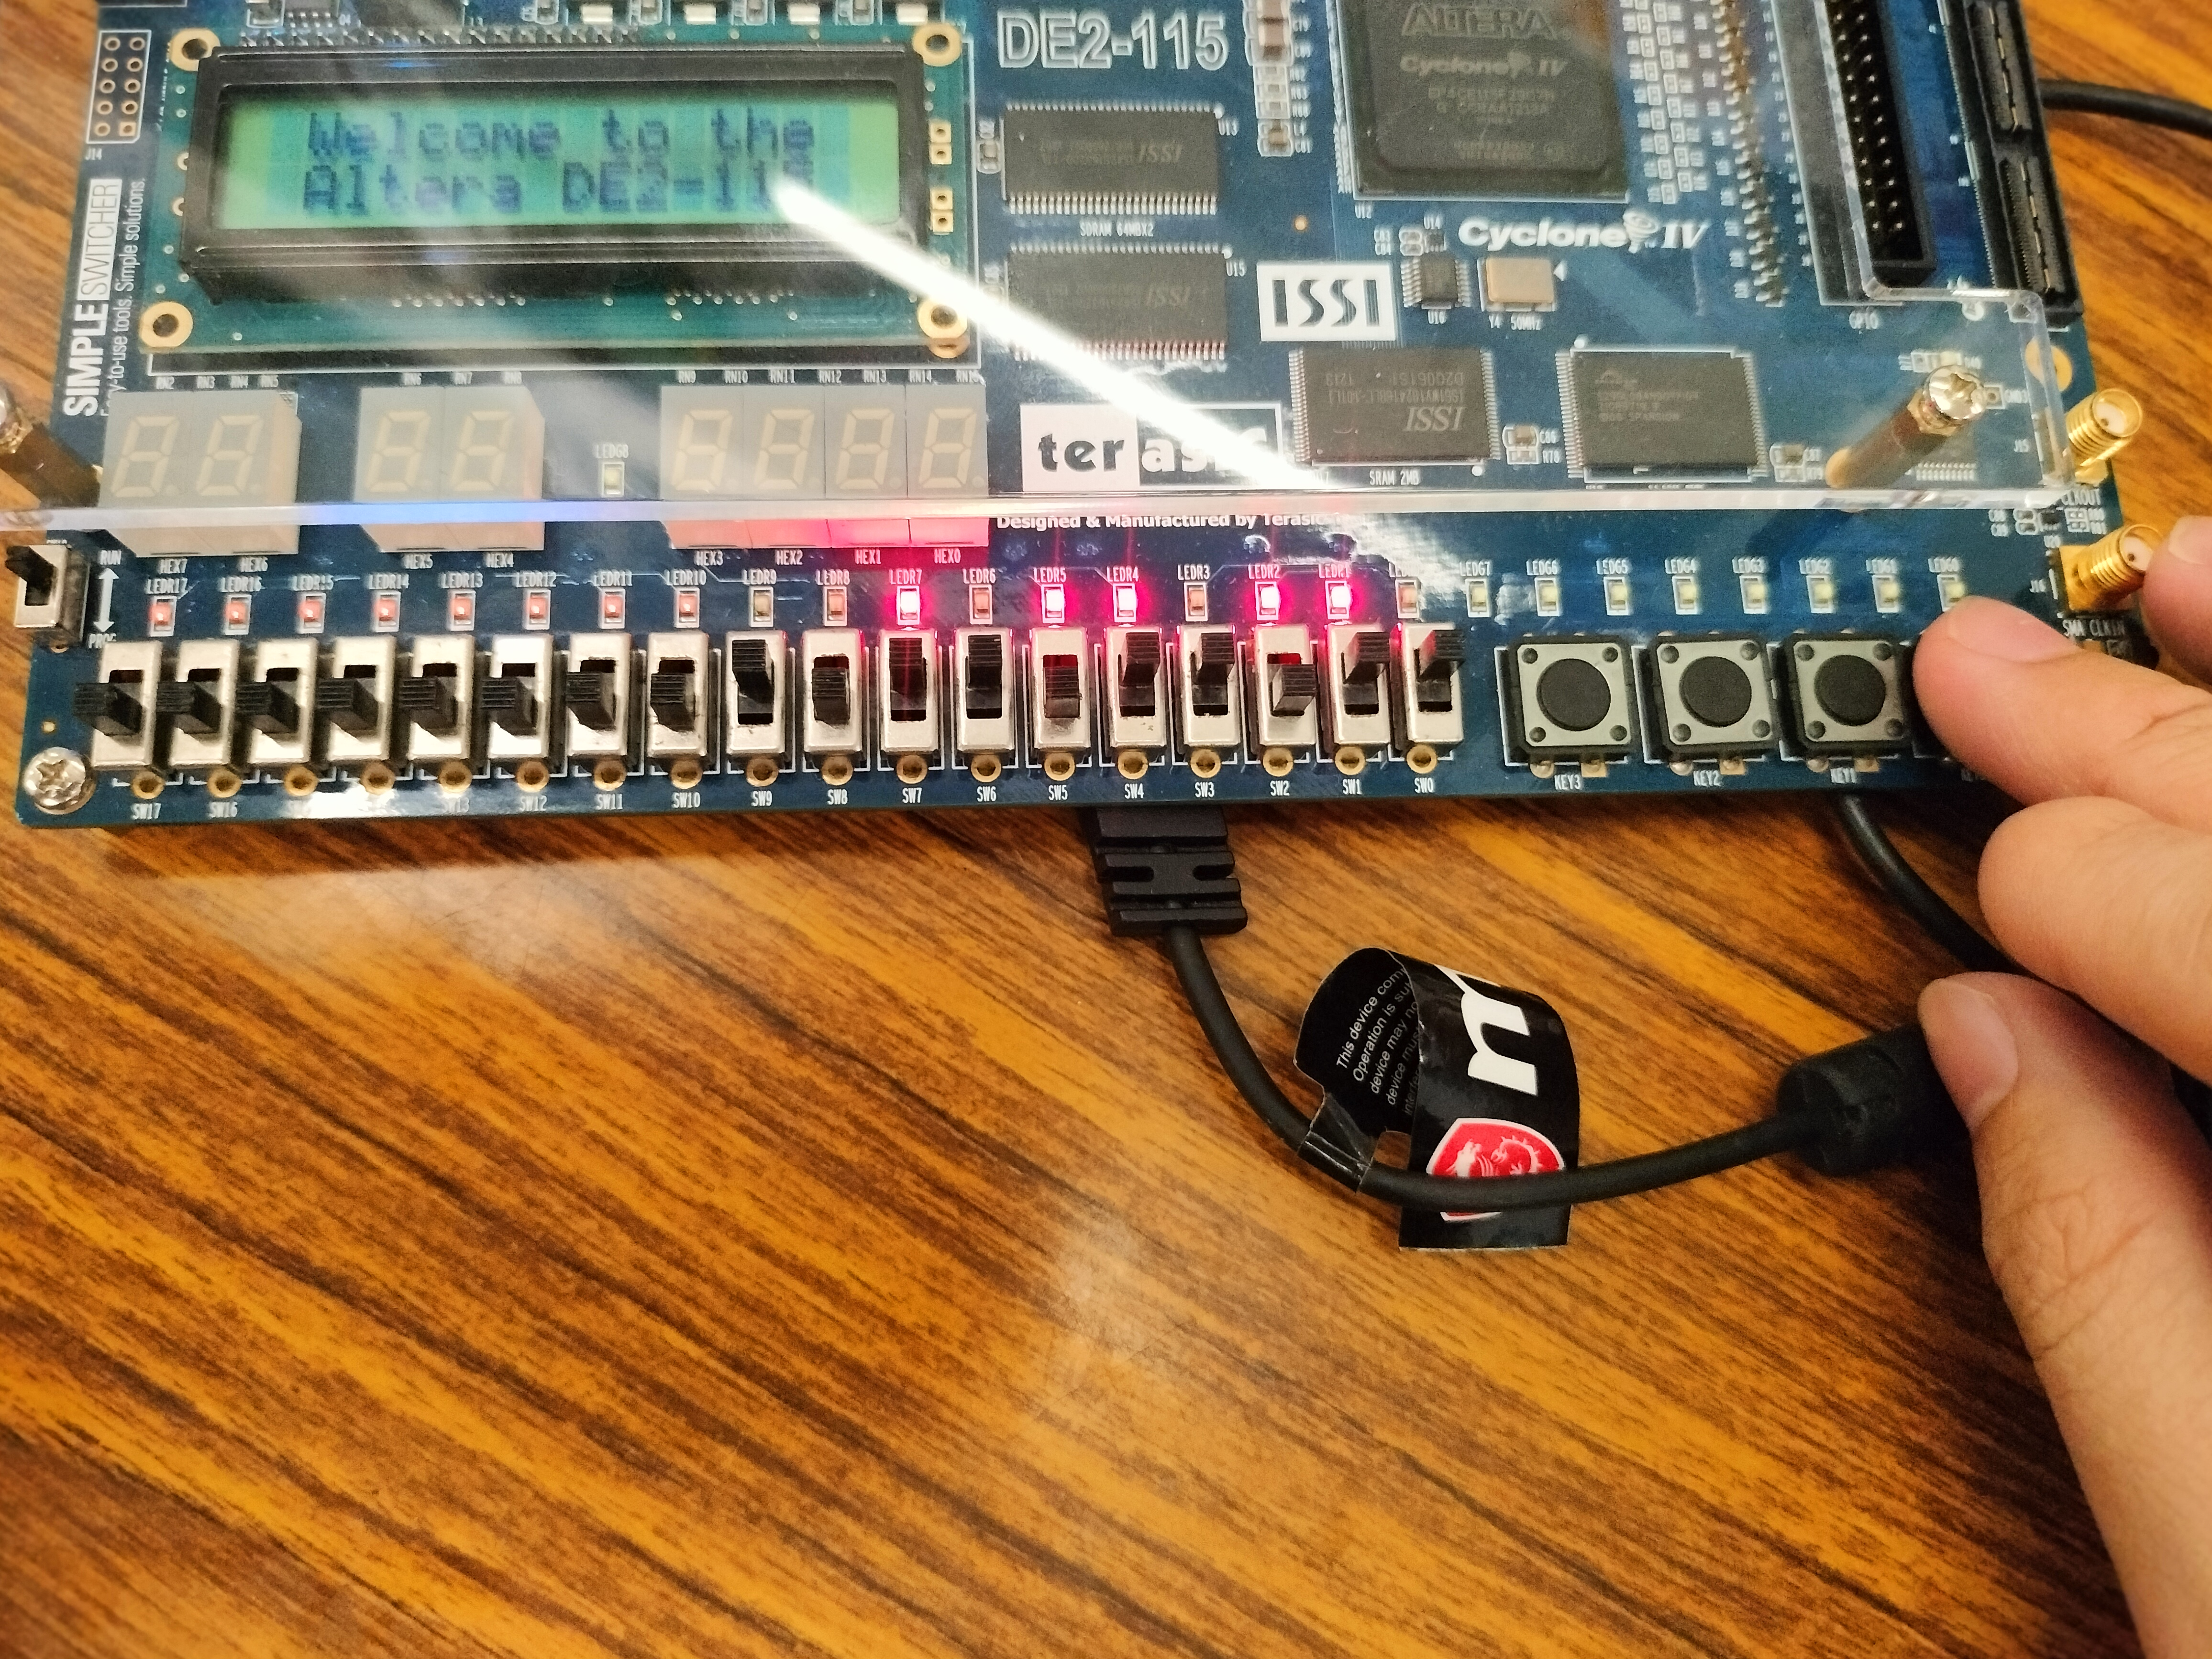
\includegraphics[width=0.5\textwidth]{./Photo/IMG20260513213633.jpg} \\
\textbf{左移過程 3}：位元持續移往 MSB。 & 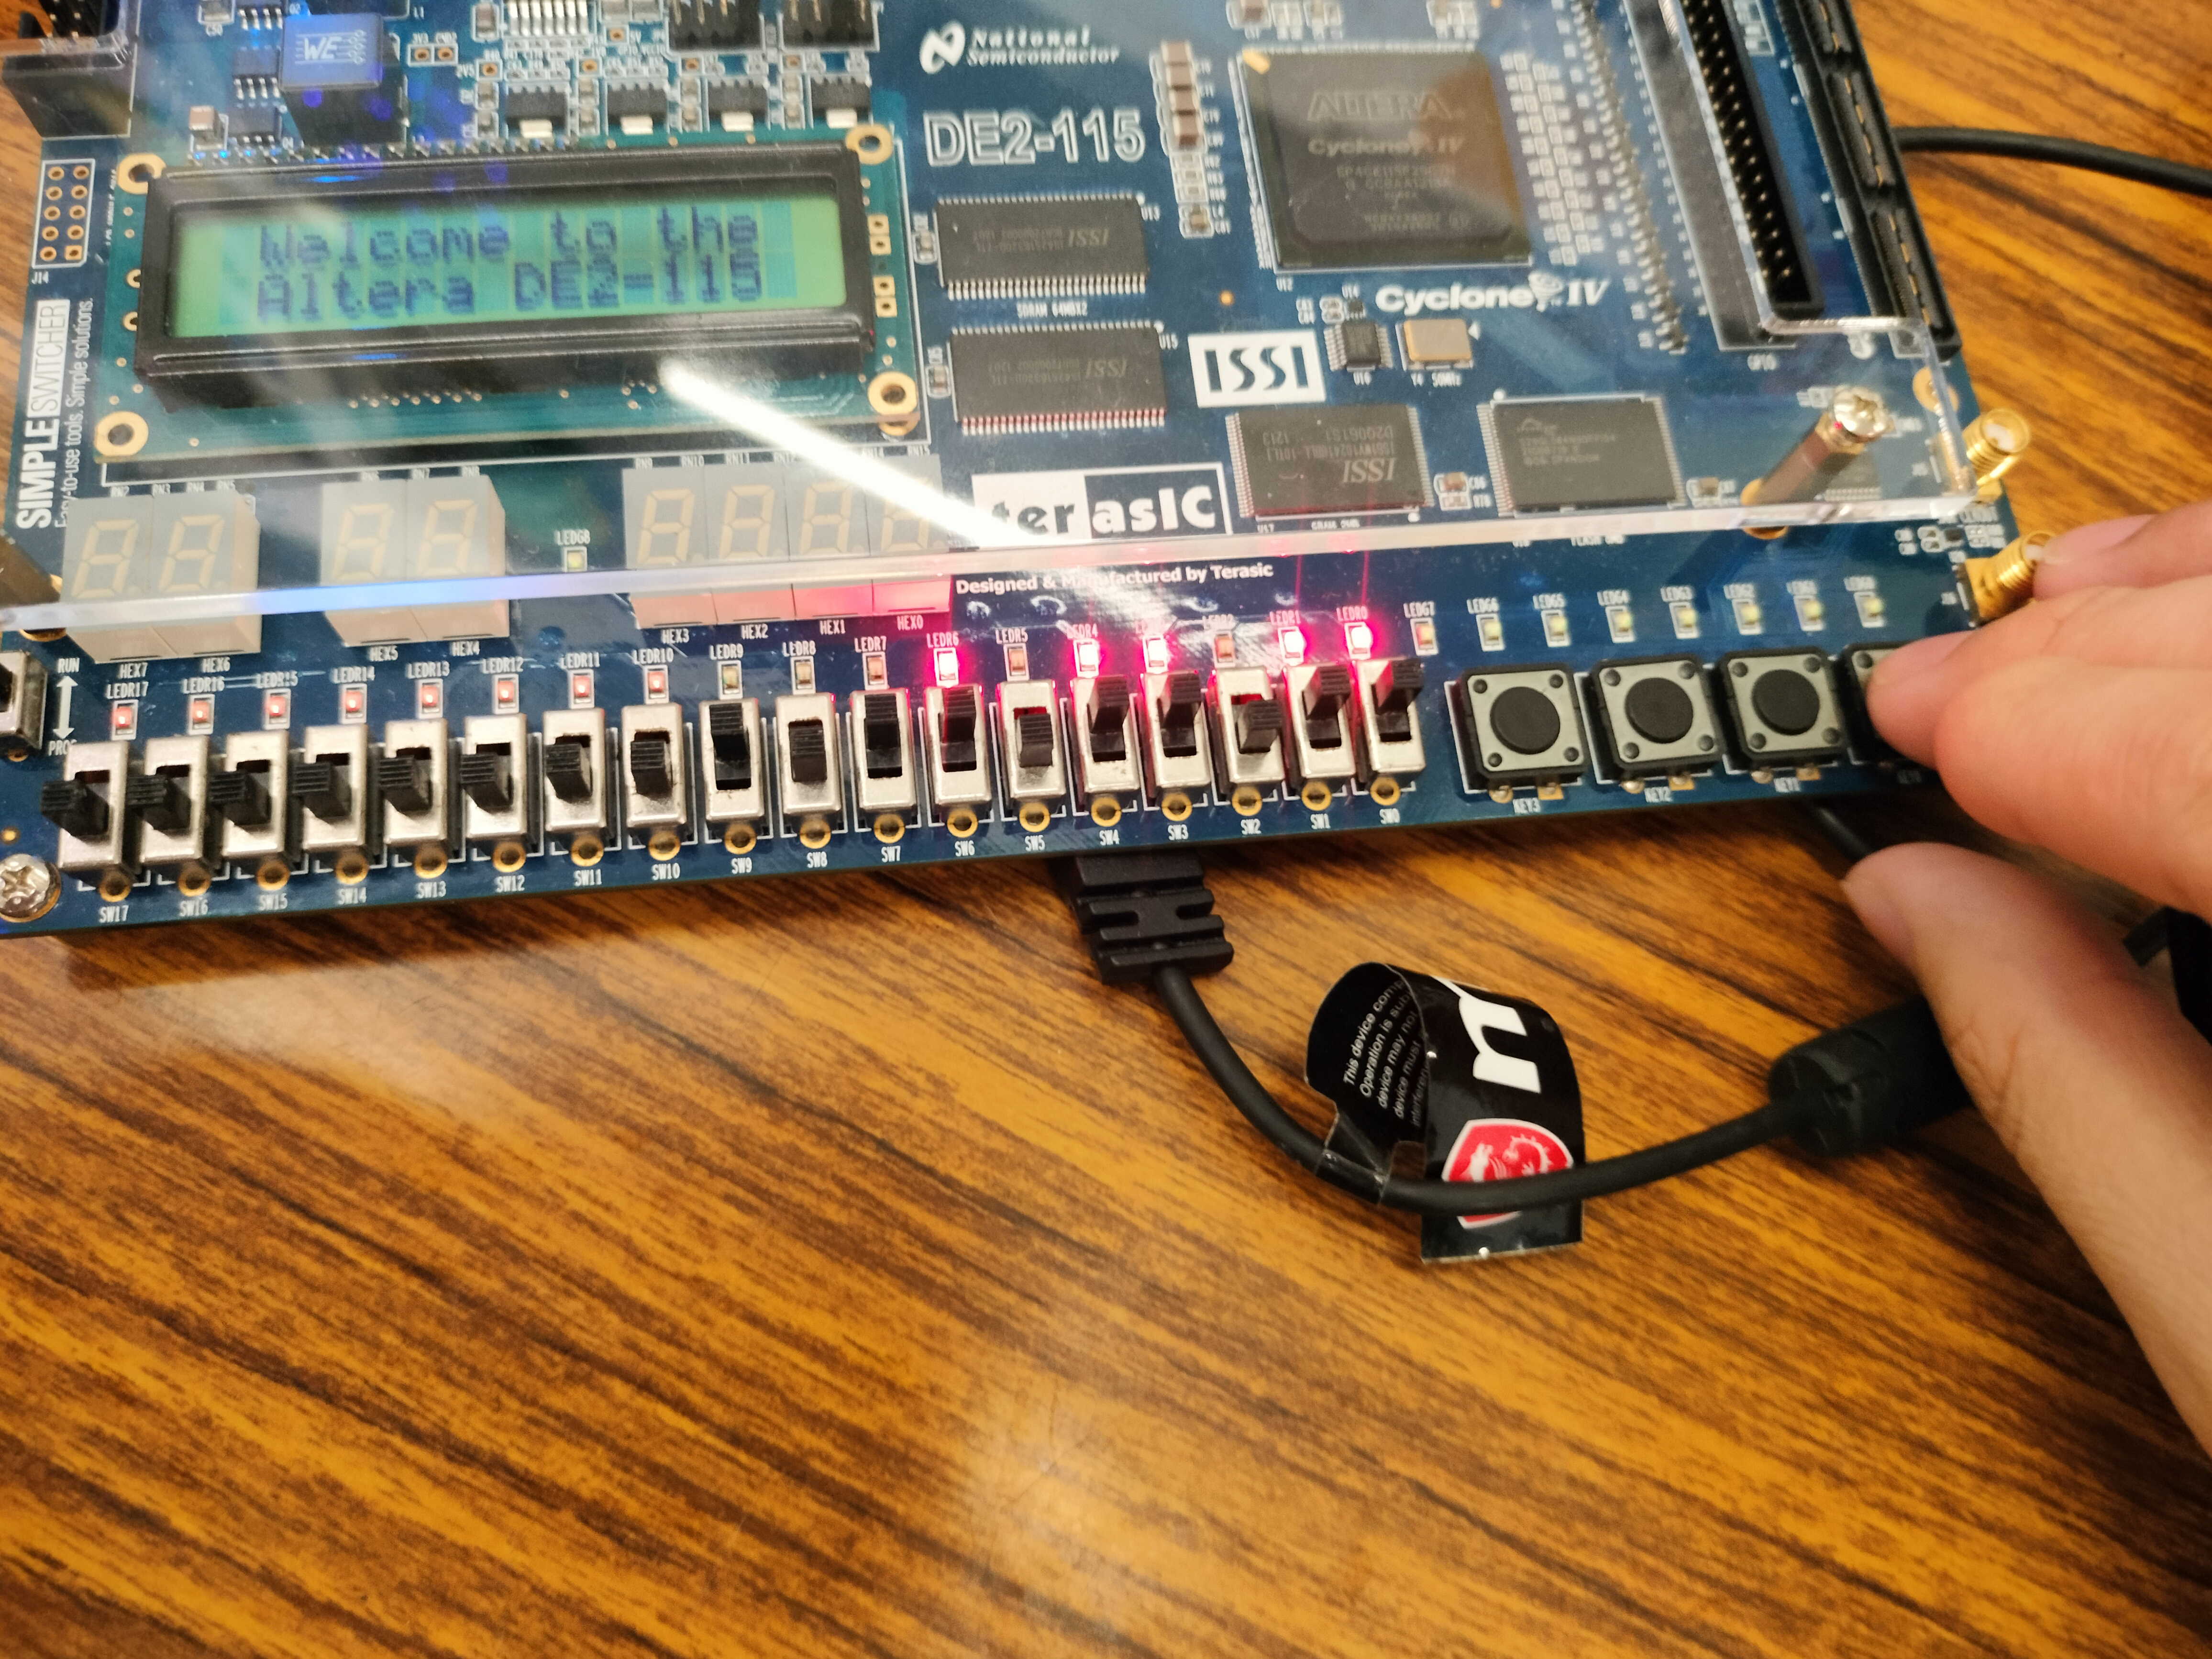
\includegraphics[width=0.5\textwidth]{./Photo/IMG20260513213706.jpg} \\
\textbf{左移過程 4}：位元即將移出邊界。 & 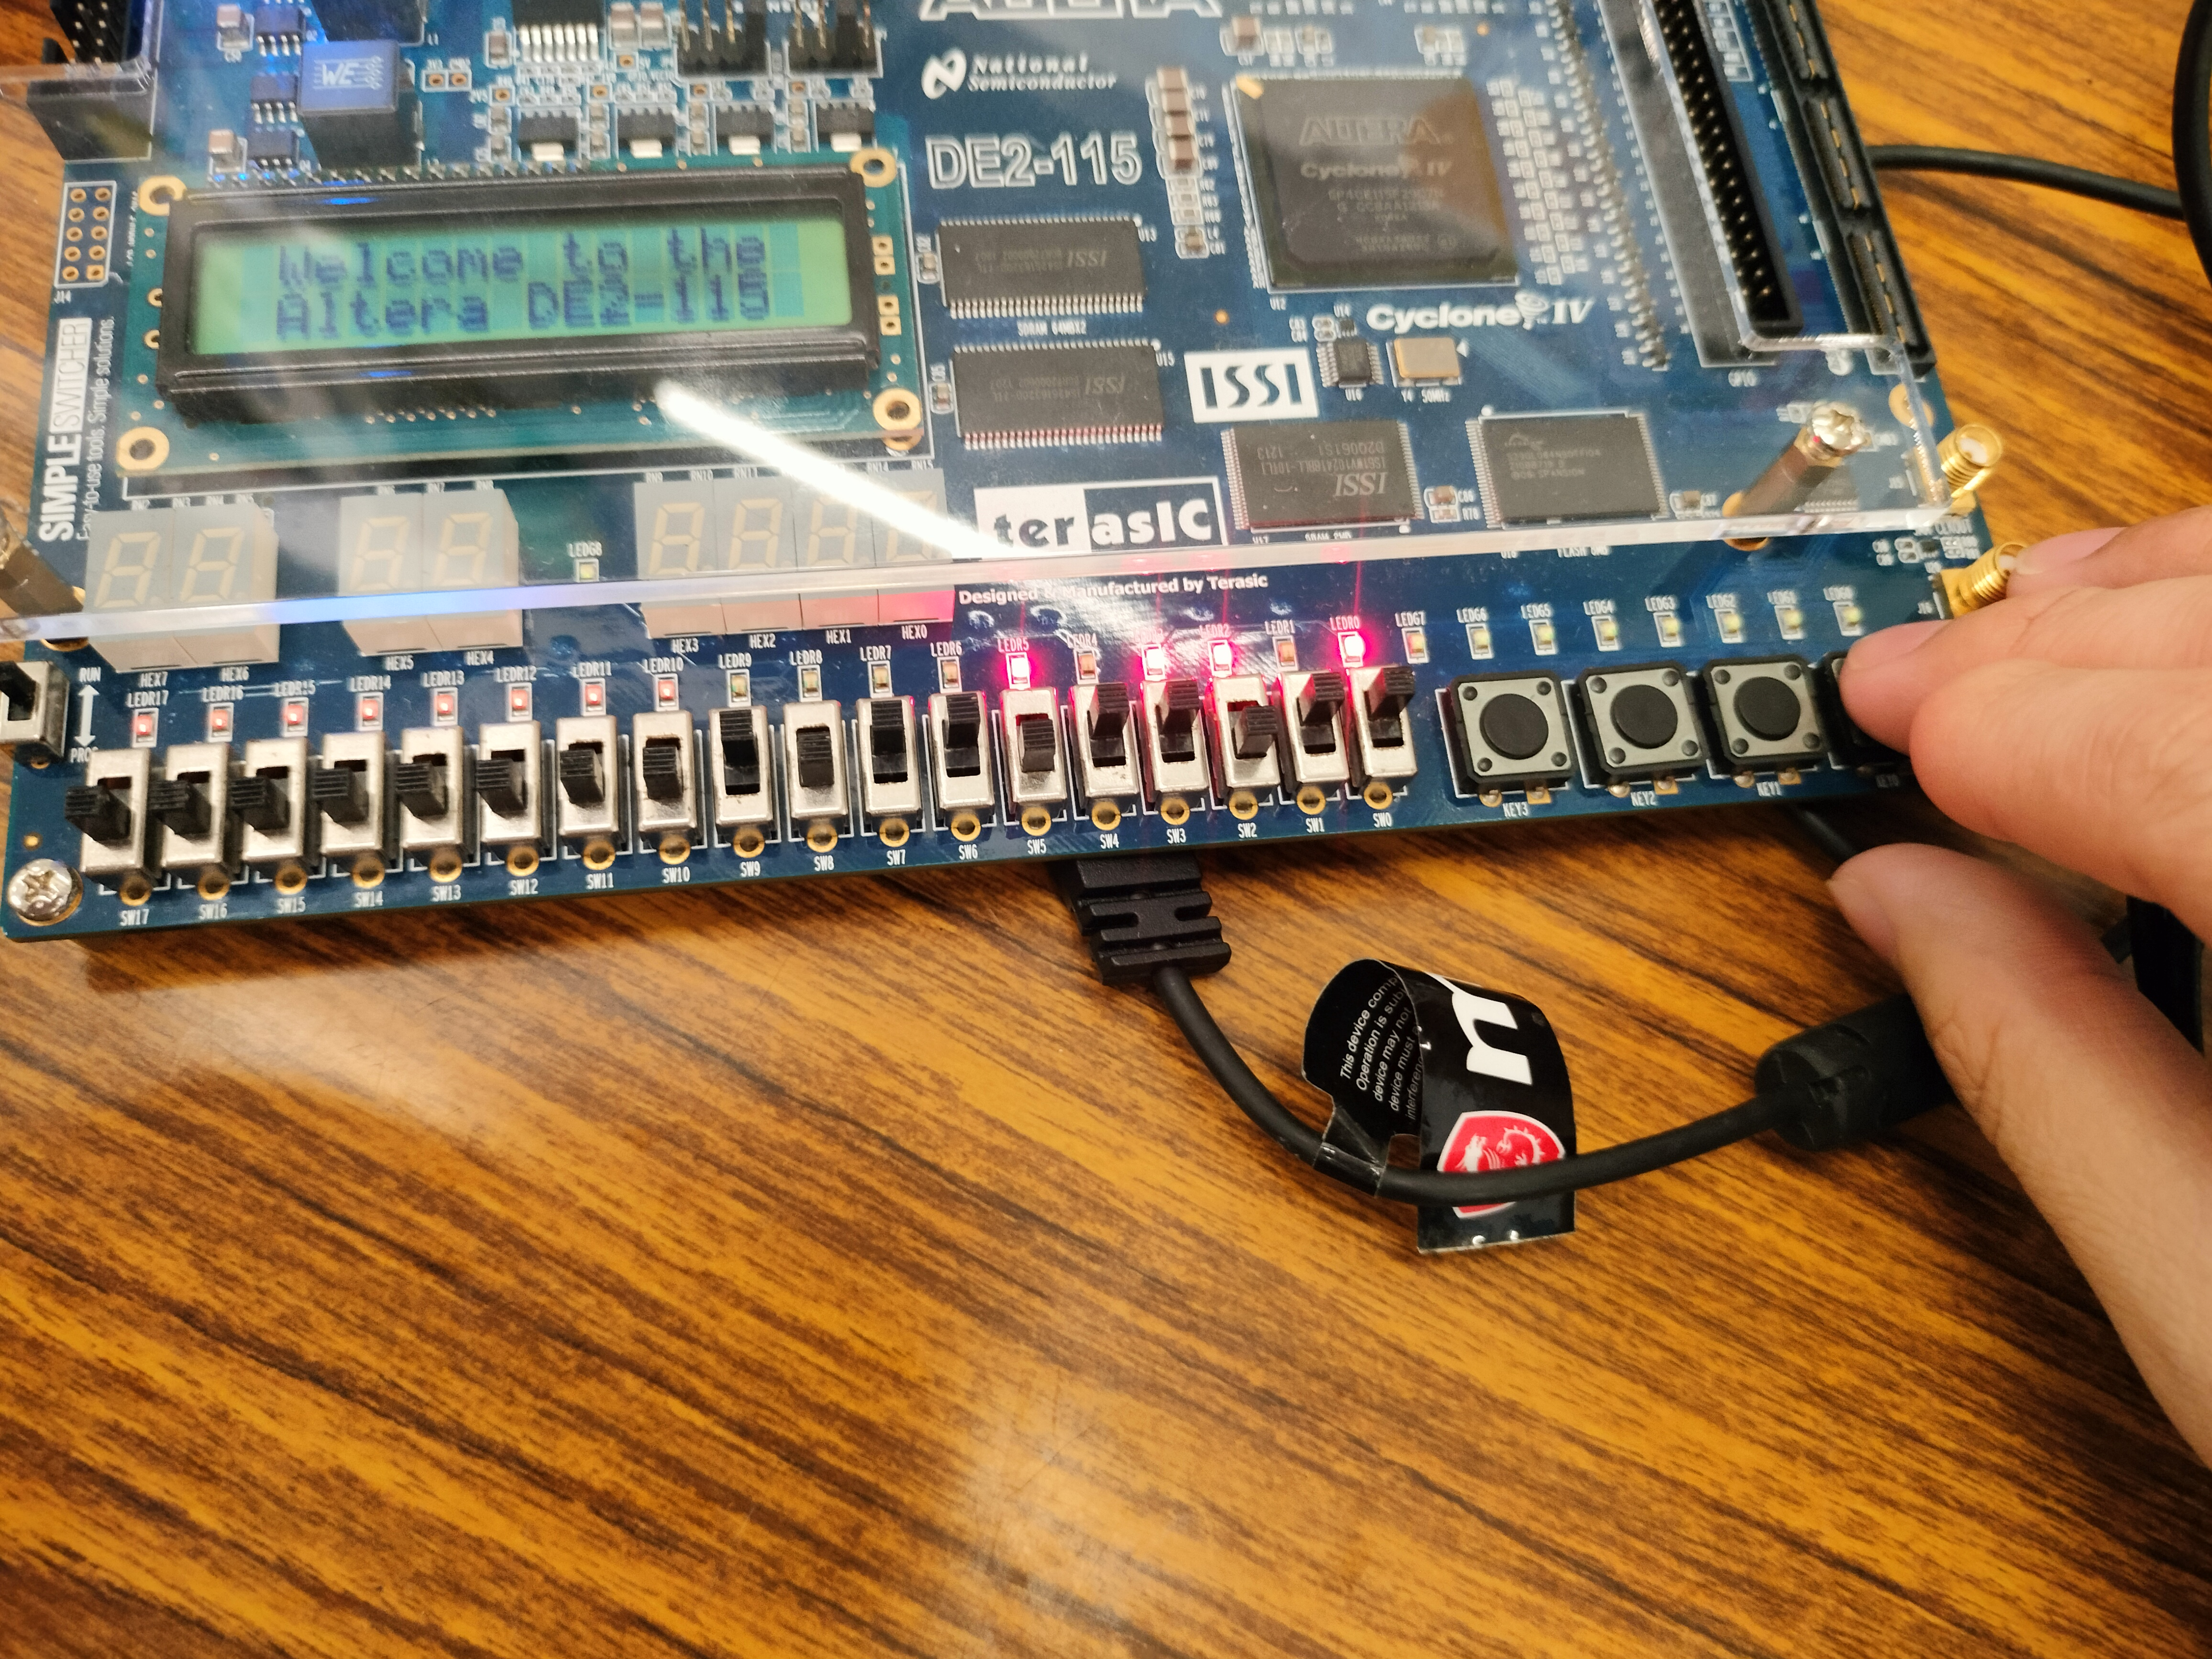
\includegraphics[width=0.5\textwidth]{./Photo/IMG20260513213711.jpg} \\
\bottomrule
\end{longtable}

\subsubsection{4. 串列輸入與連續位移 (SDI \& Shift)}
\begin{longtable}{p{5cm} c}
\toprule
狀態描述 & 實體照片 \\
\midrule
\textbf{SDI 輸入 1}：設定 SW13 (sdi)，觀察新位元從 LSB 進入。 & 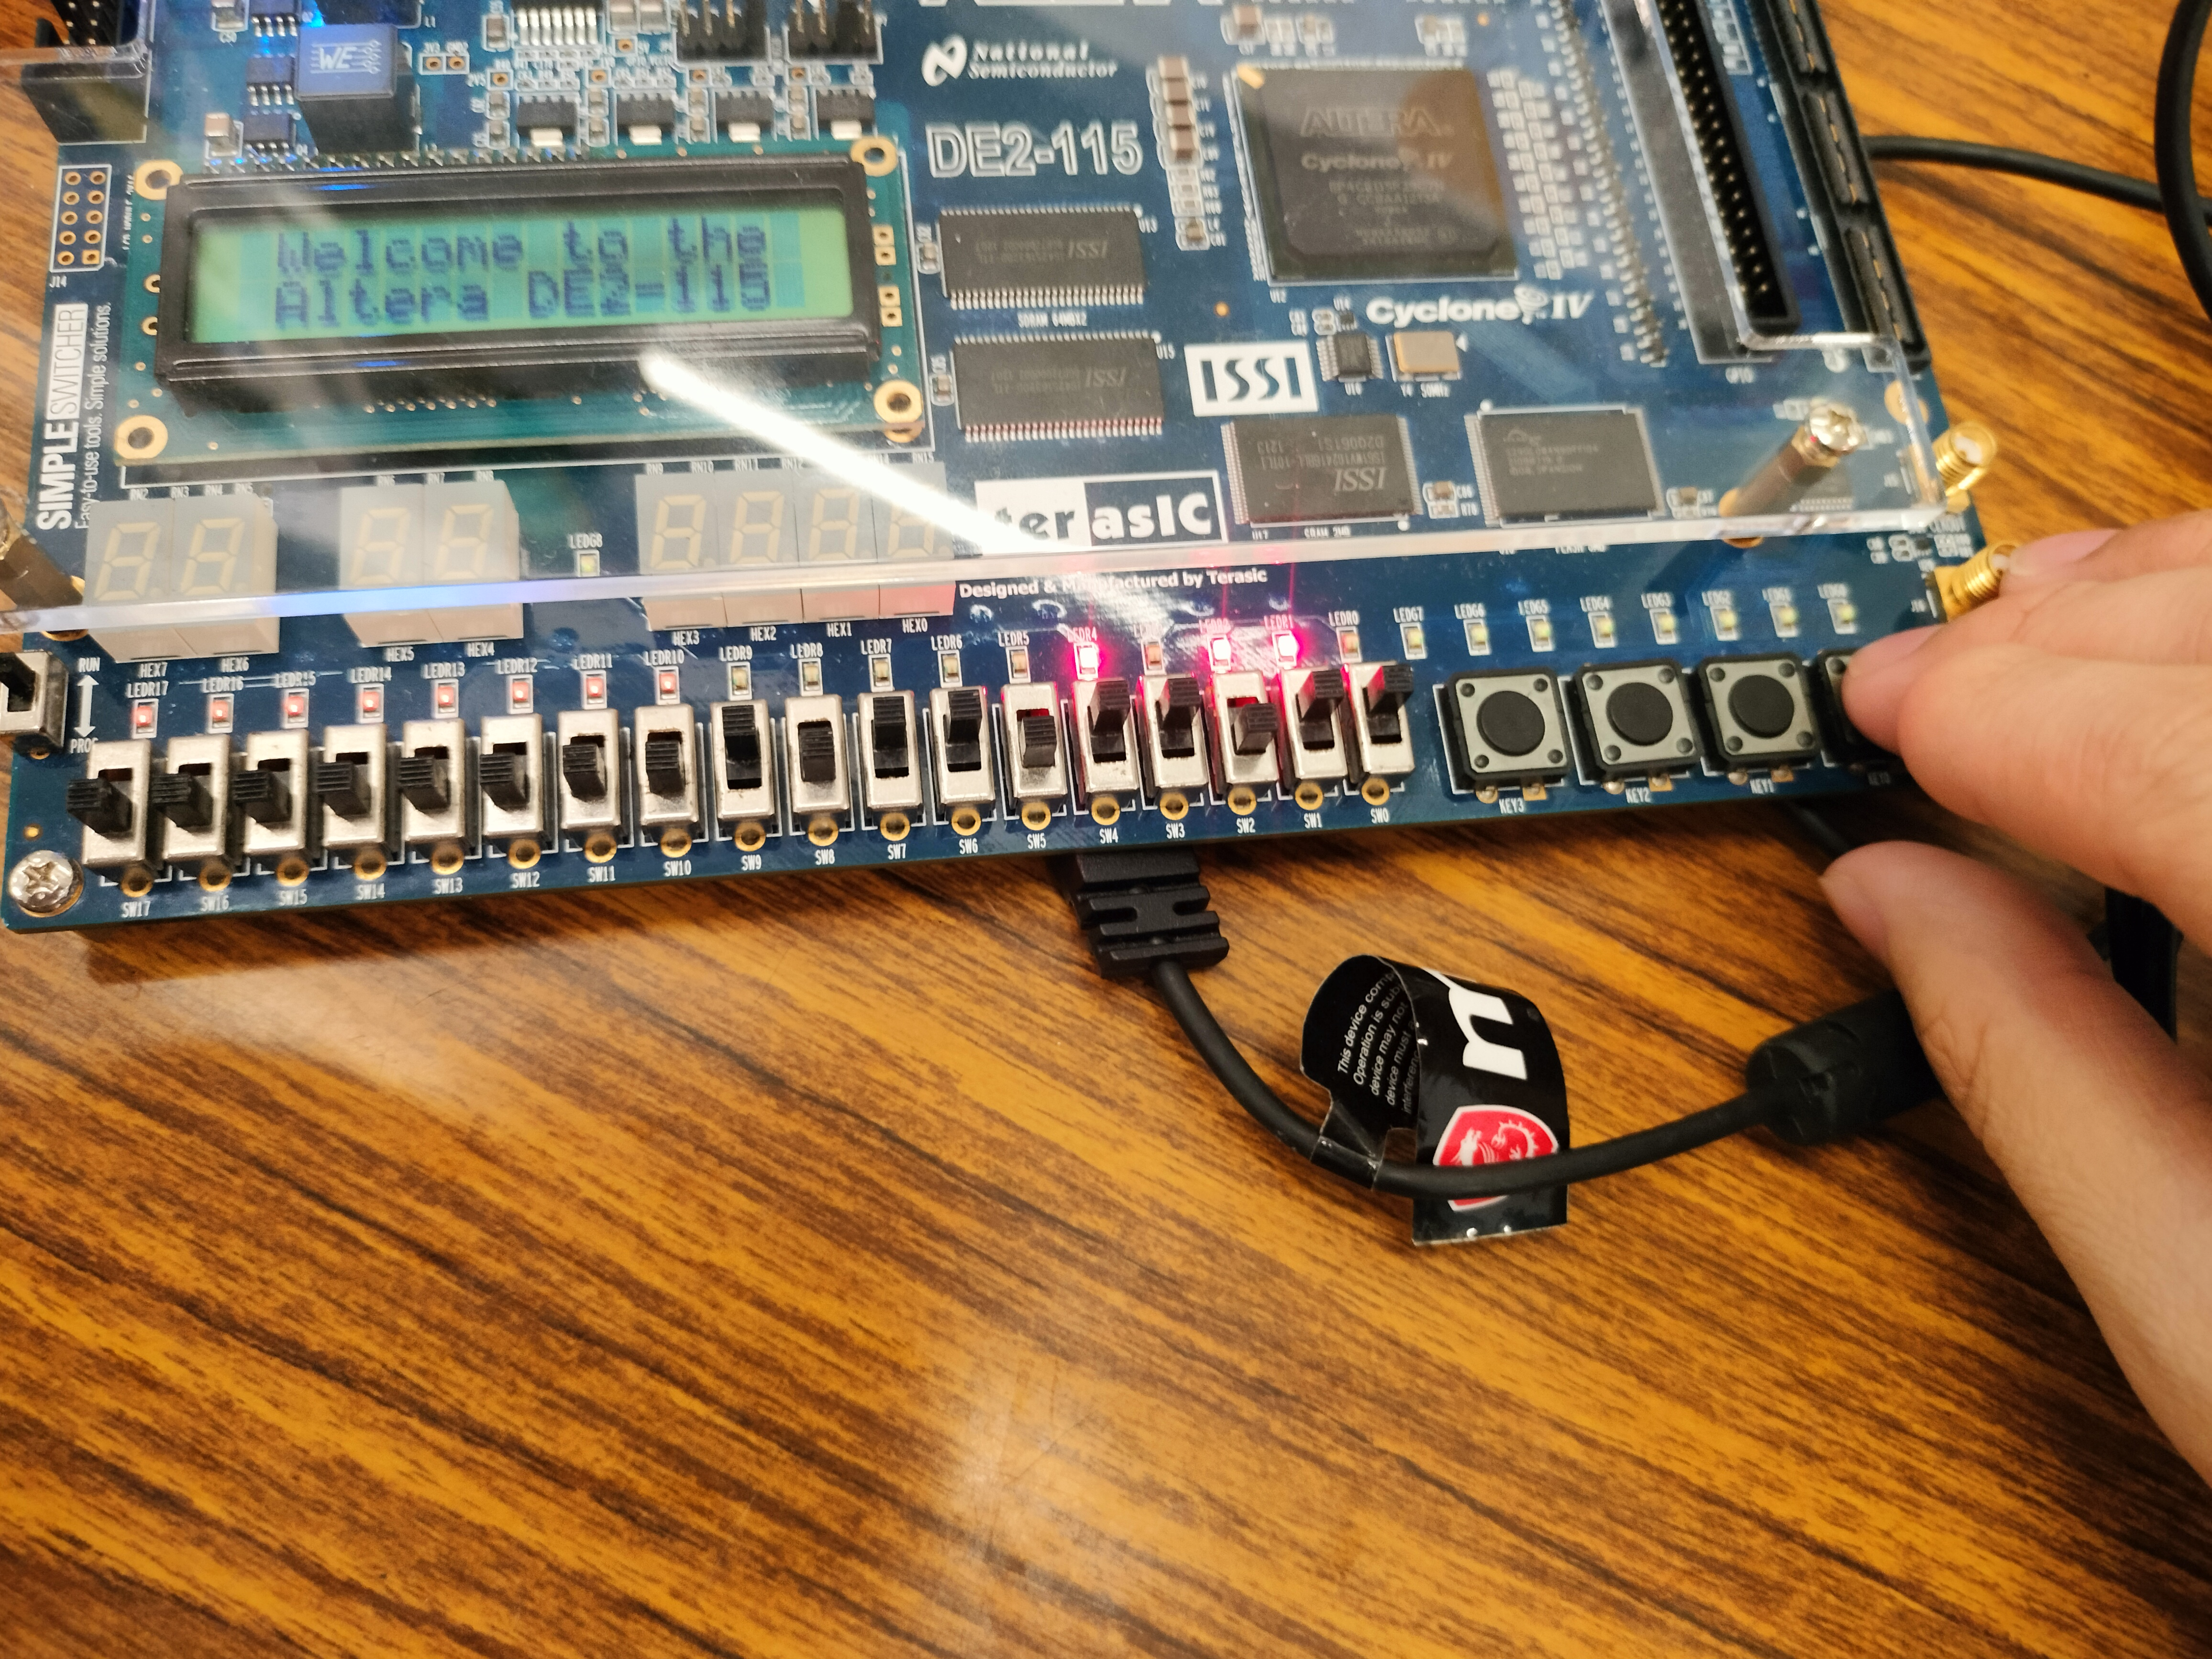
\includegraphics[width=0.5\textwidth]{./Photo/IMG20260513213716.jpg} \\
\textbf{SDI 輸入 2}：連續位移使 sdi 填滿低位元。 & 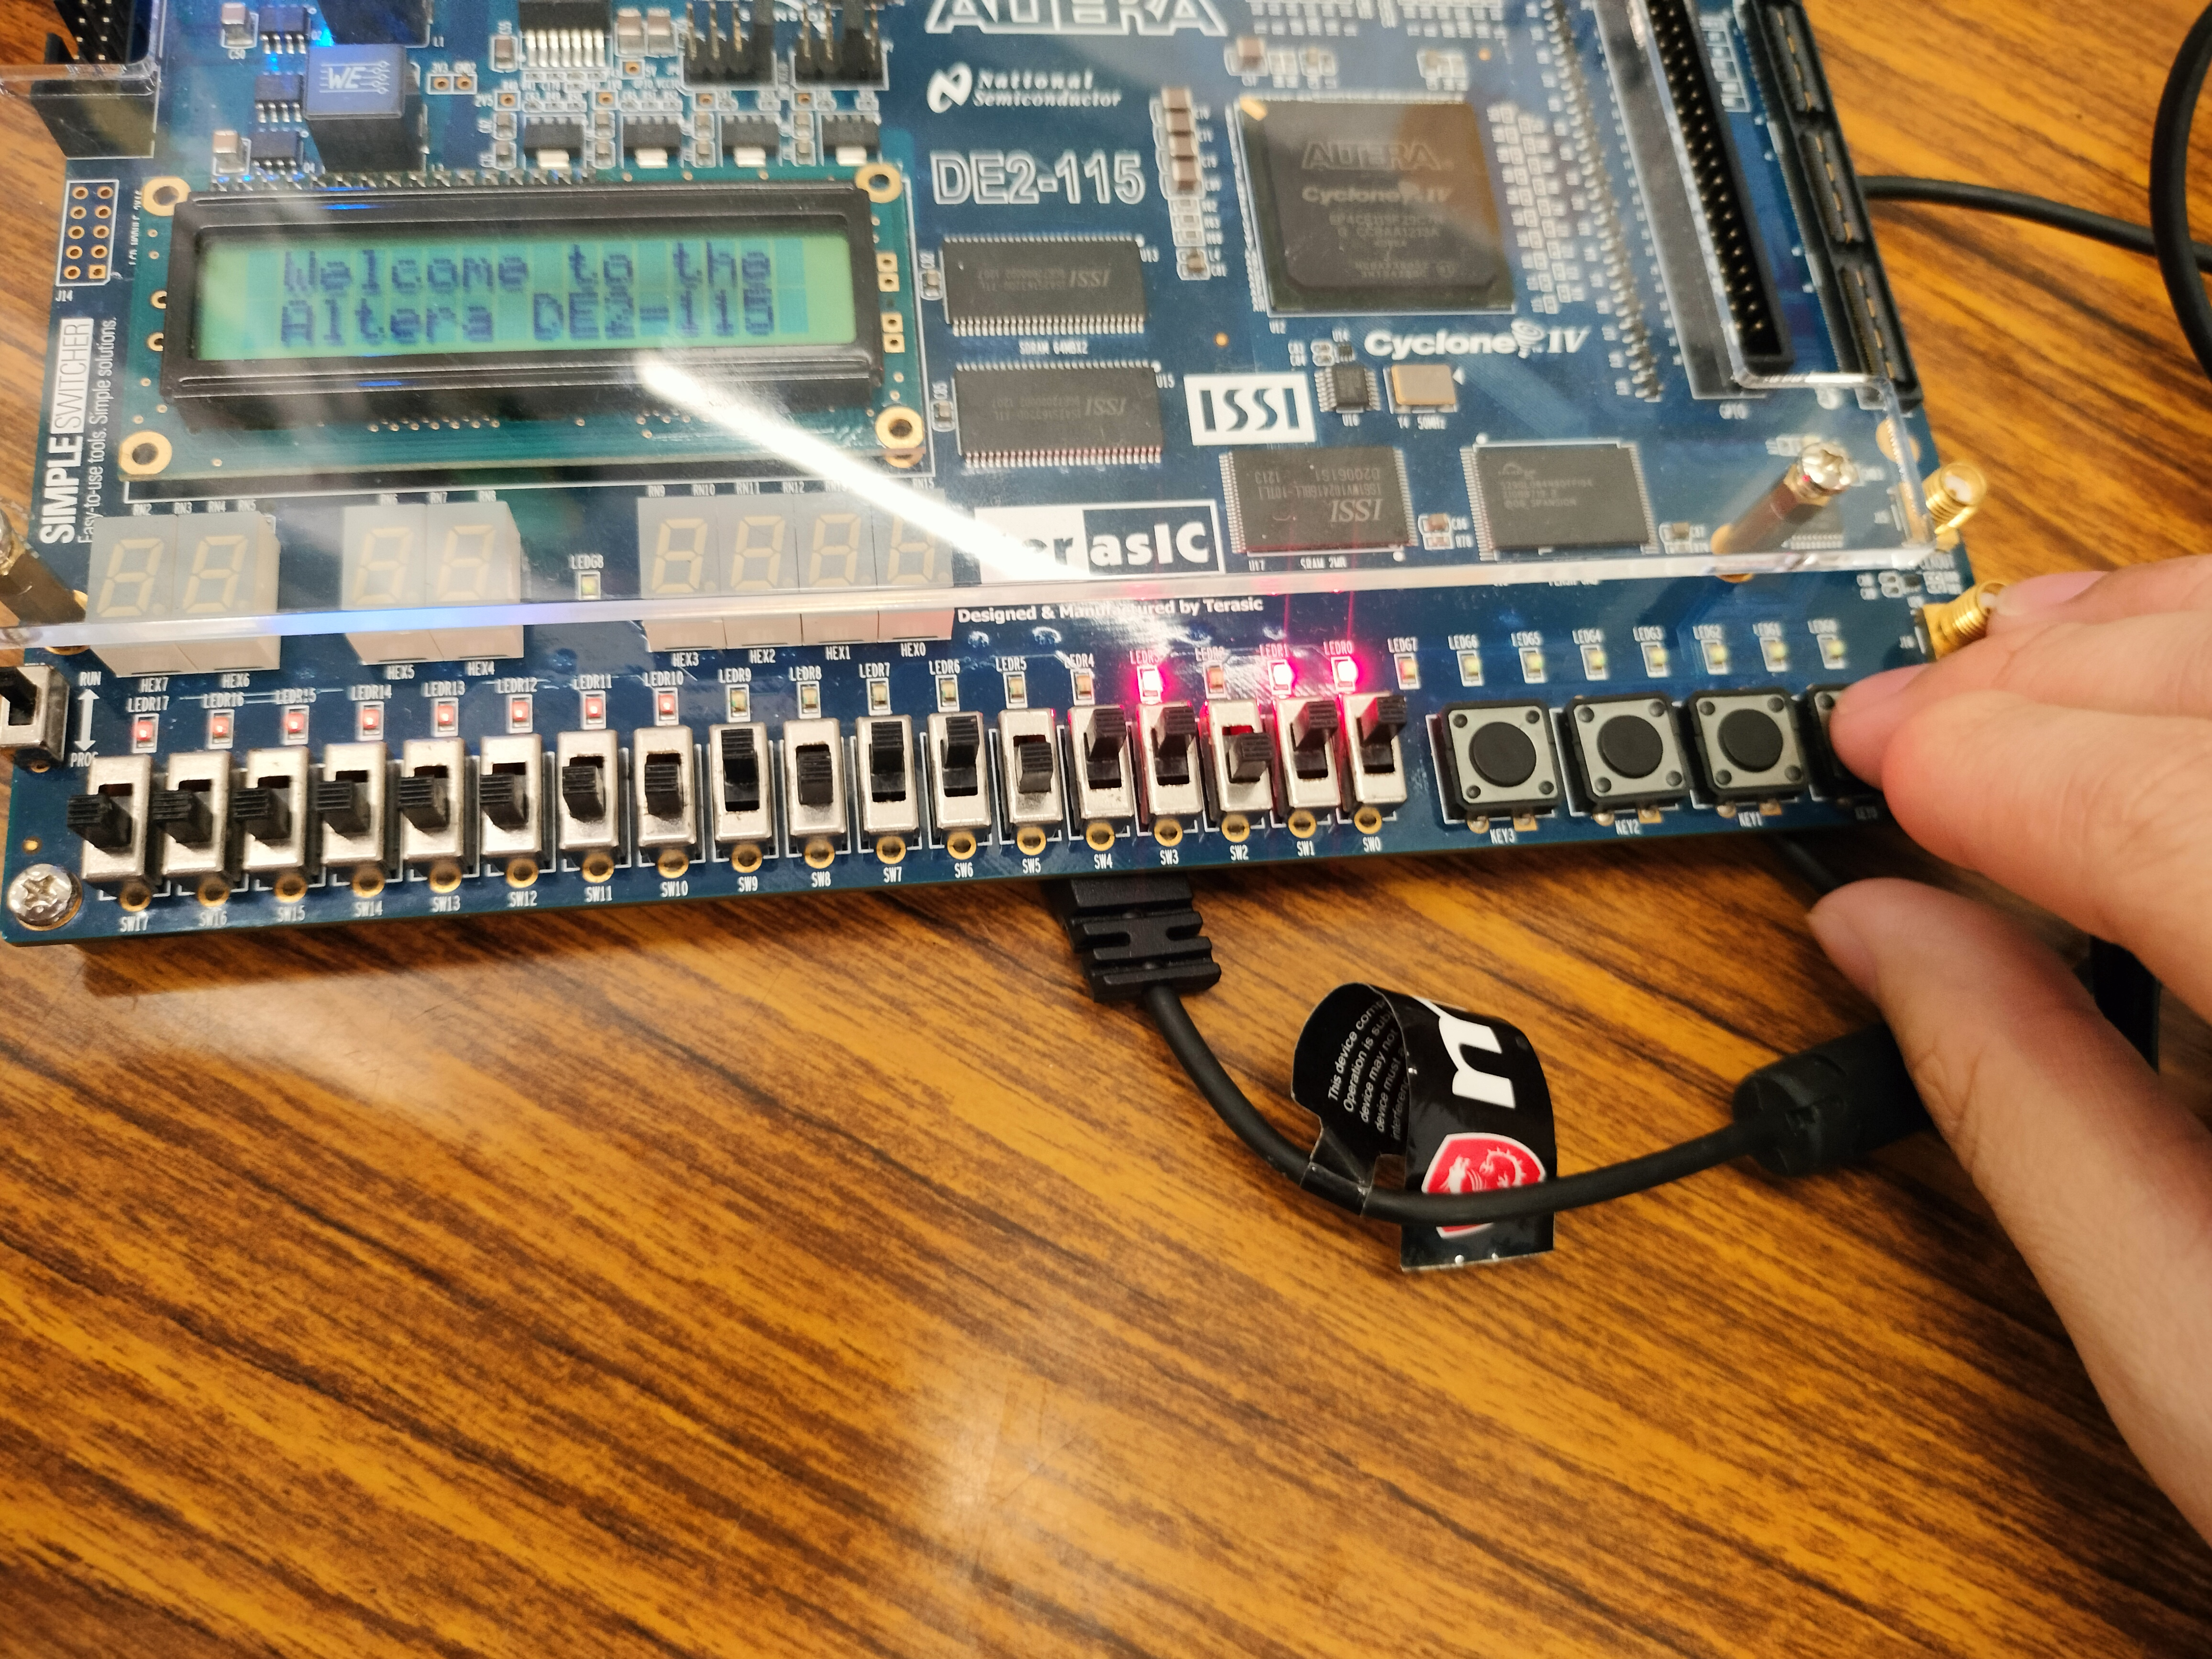
\includegraphics[width=0.5\textwidth]{./Photo/IMG20260513213719.jpg} \\
\textbf{SDI 輸入 3}：模式完整移入之狀態。 & 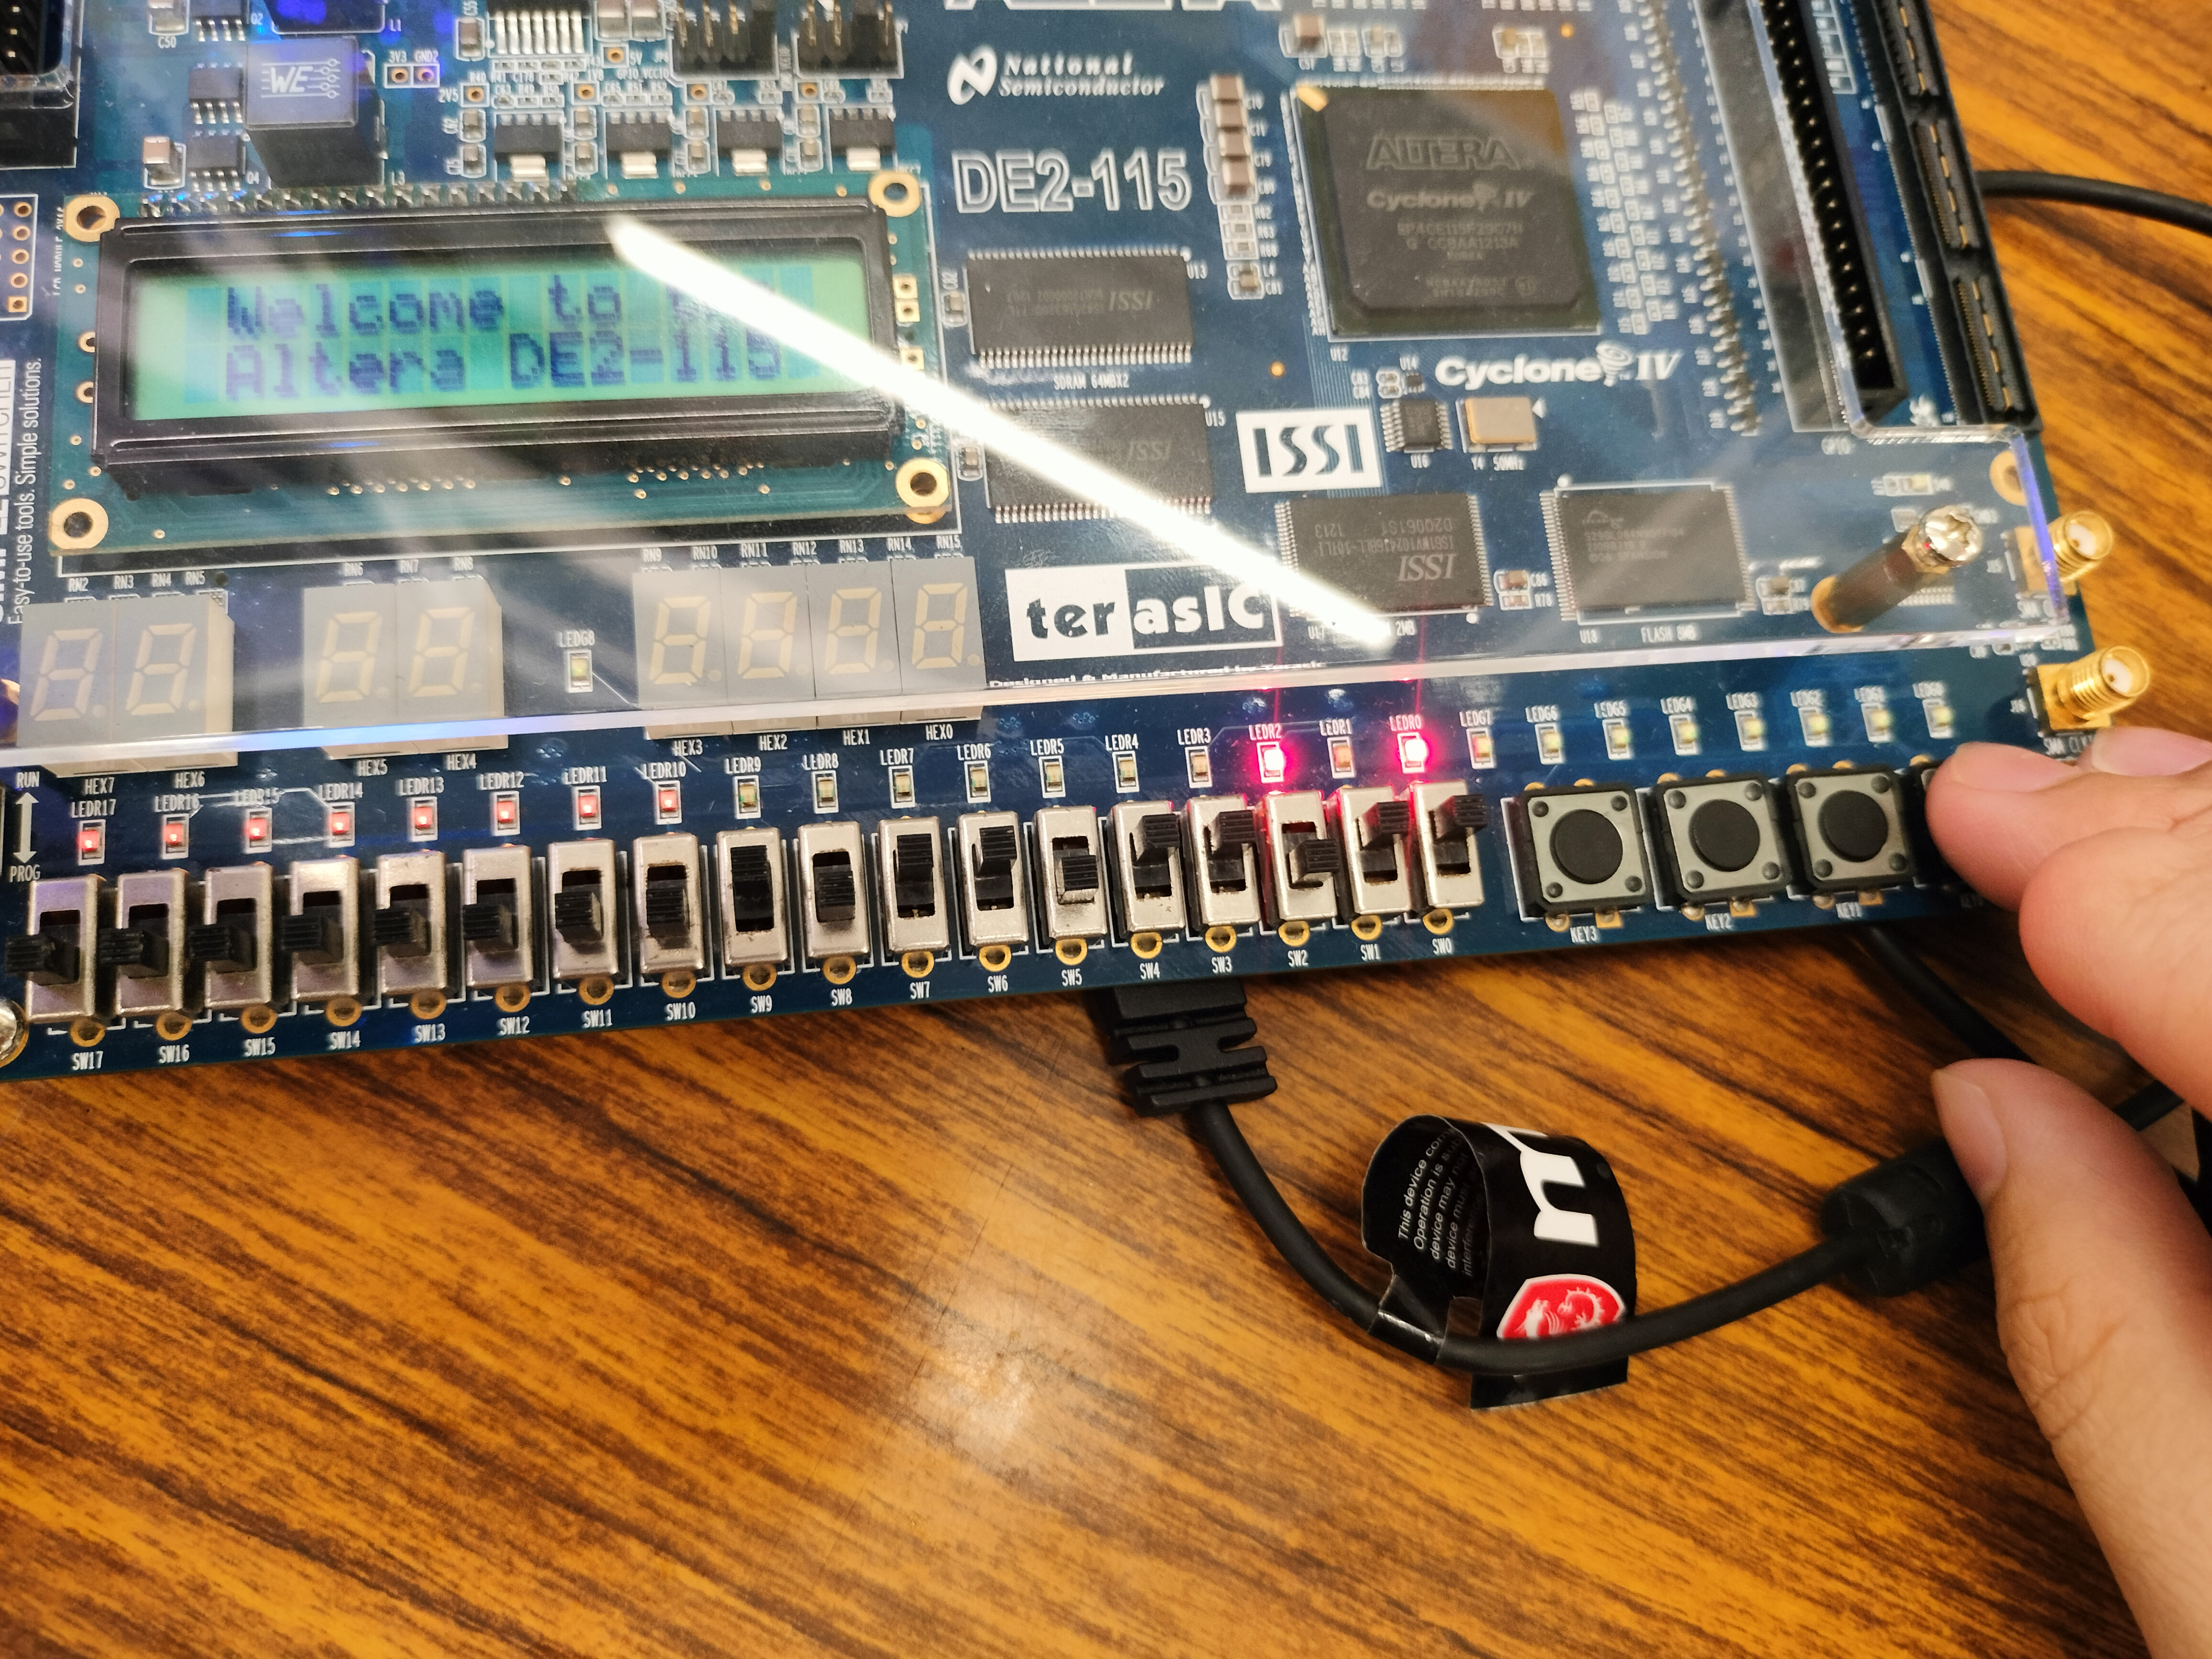
\includegraphics[width=0.5\textwidth]{./Photo/IMG20260513213753.jpg} \\
\textbf{位移序列 A}：展示連續位移的連貫性。 & 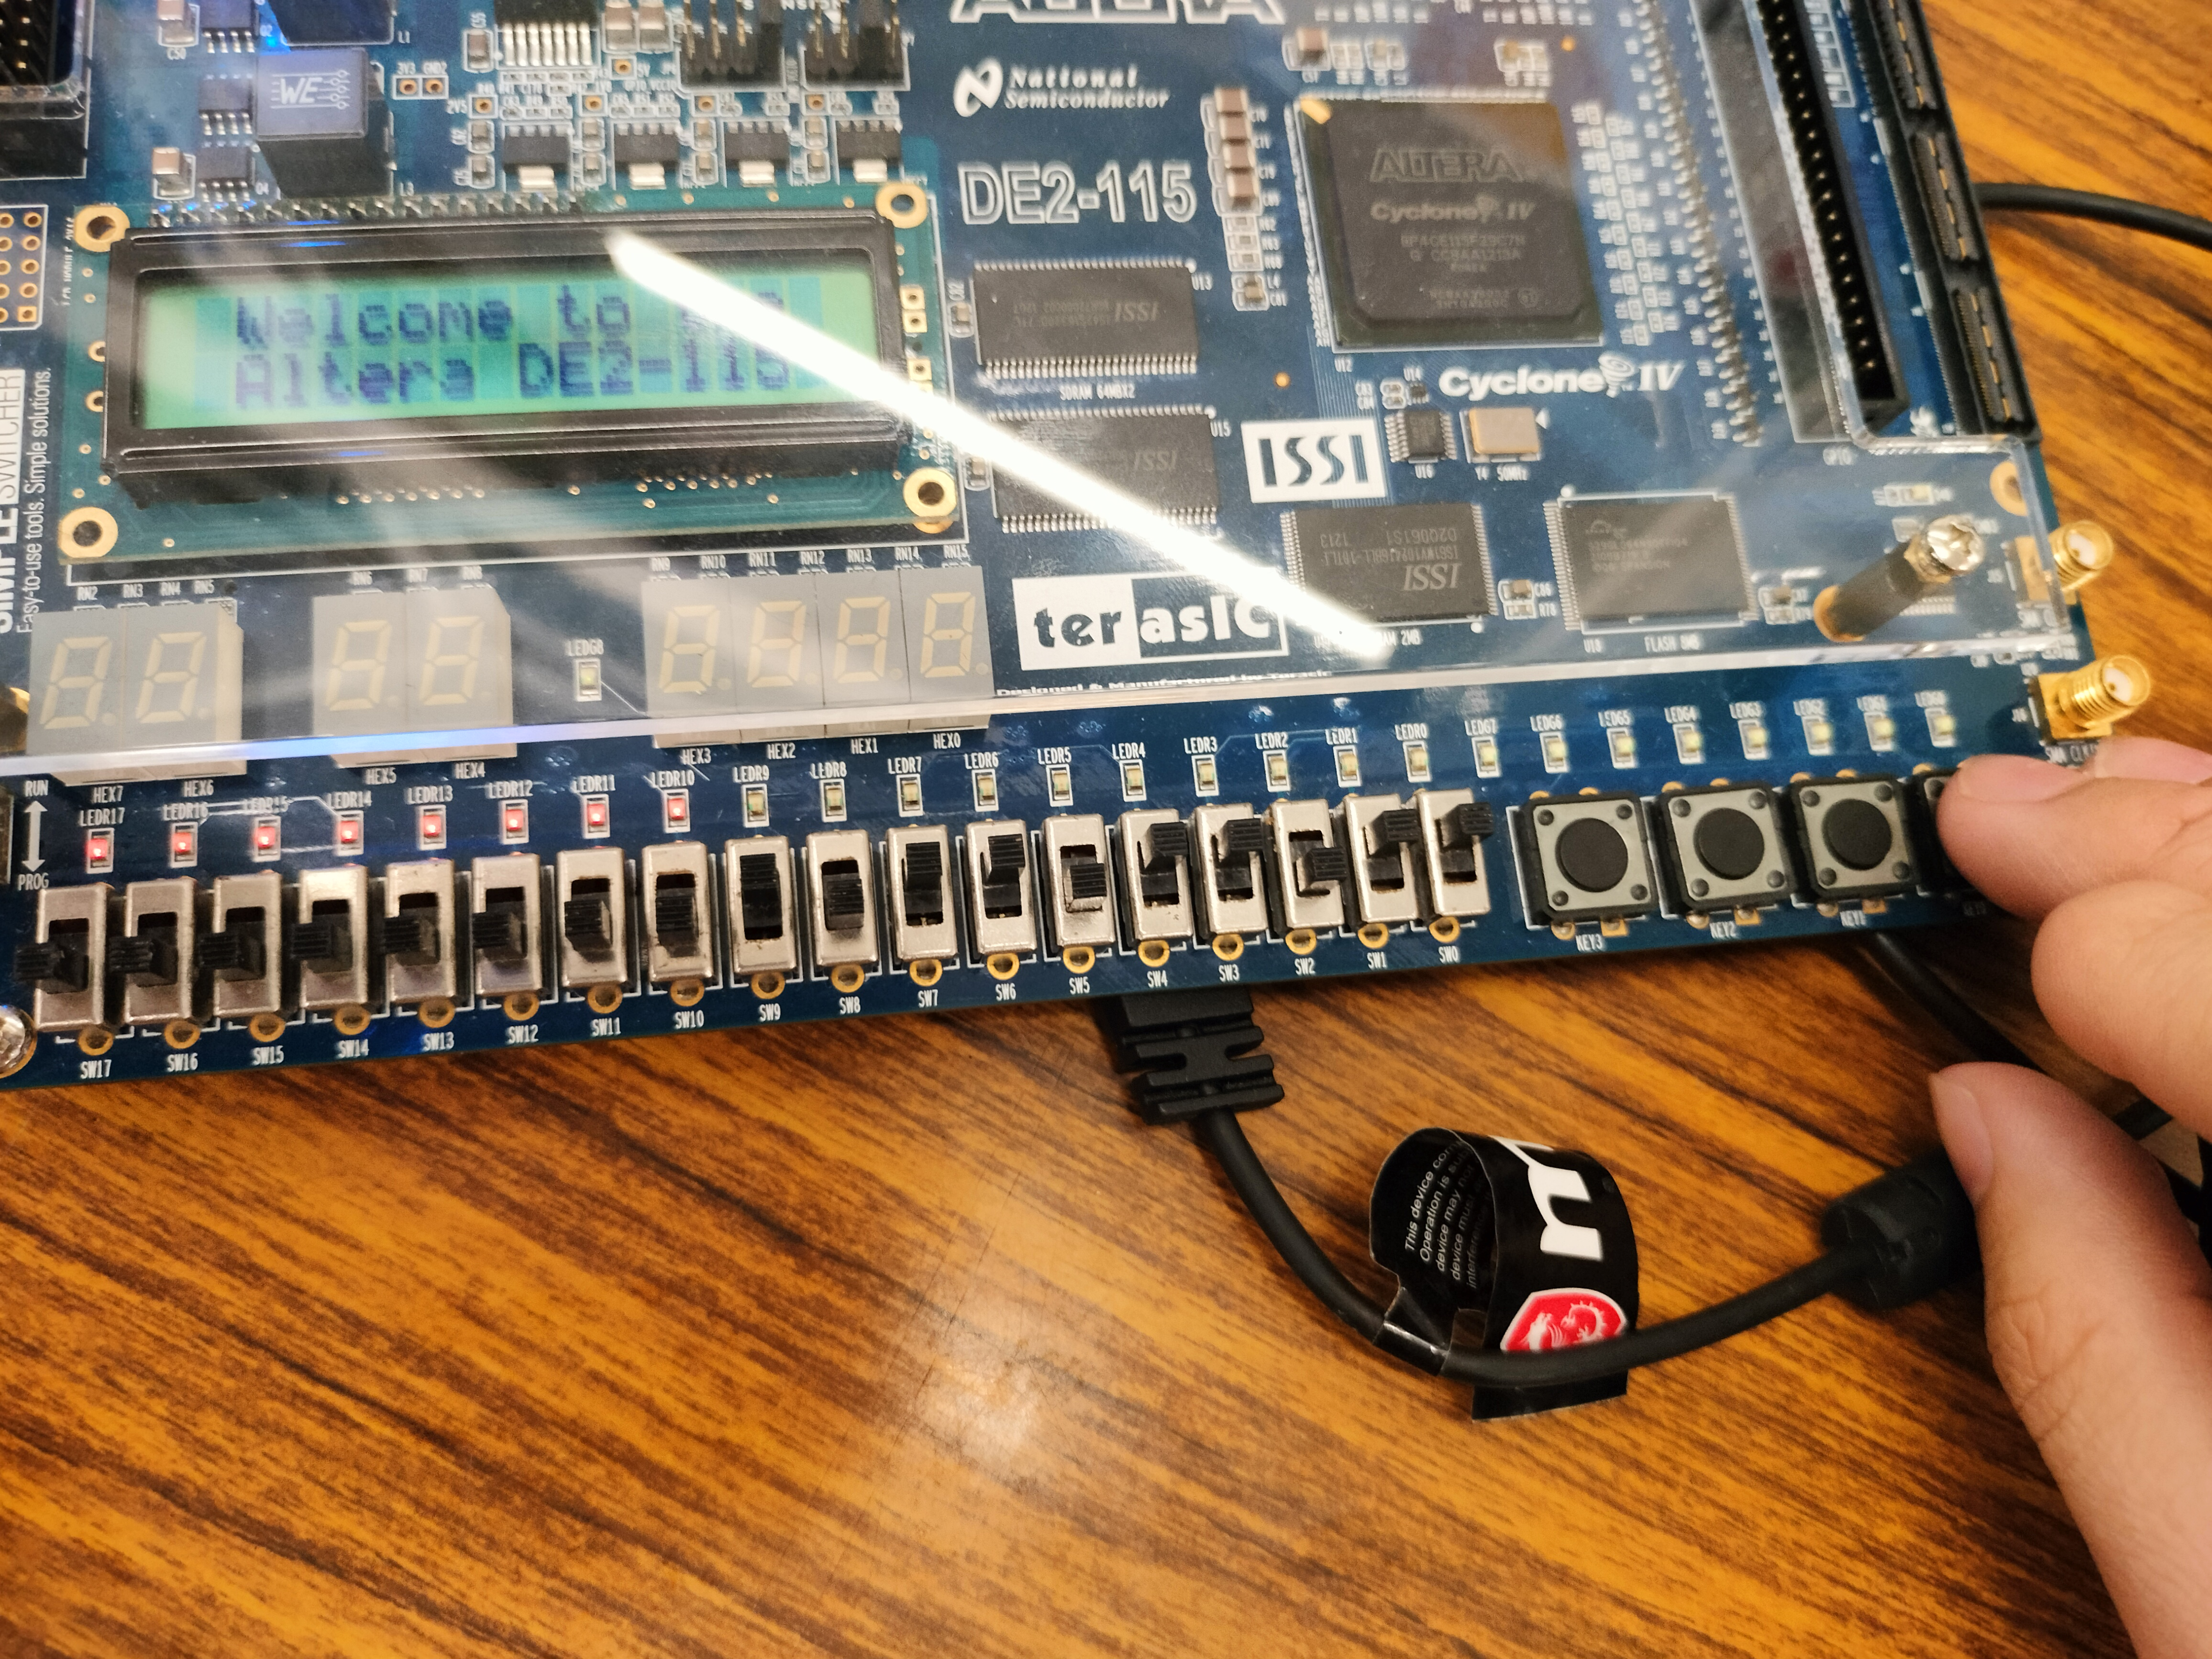
\includegraphics[width=0.5\textwidth]{./Photo/IMG20260513213801.jpg} \\
\textbf{位移序列 B}：展示連續位移的連貫性。 & 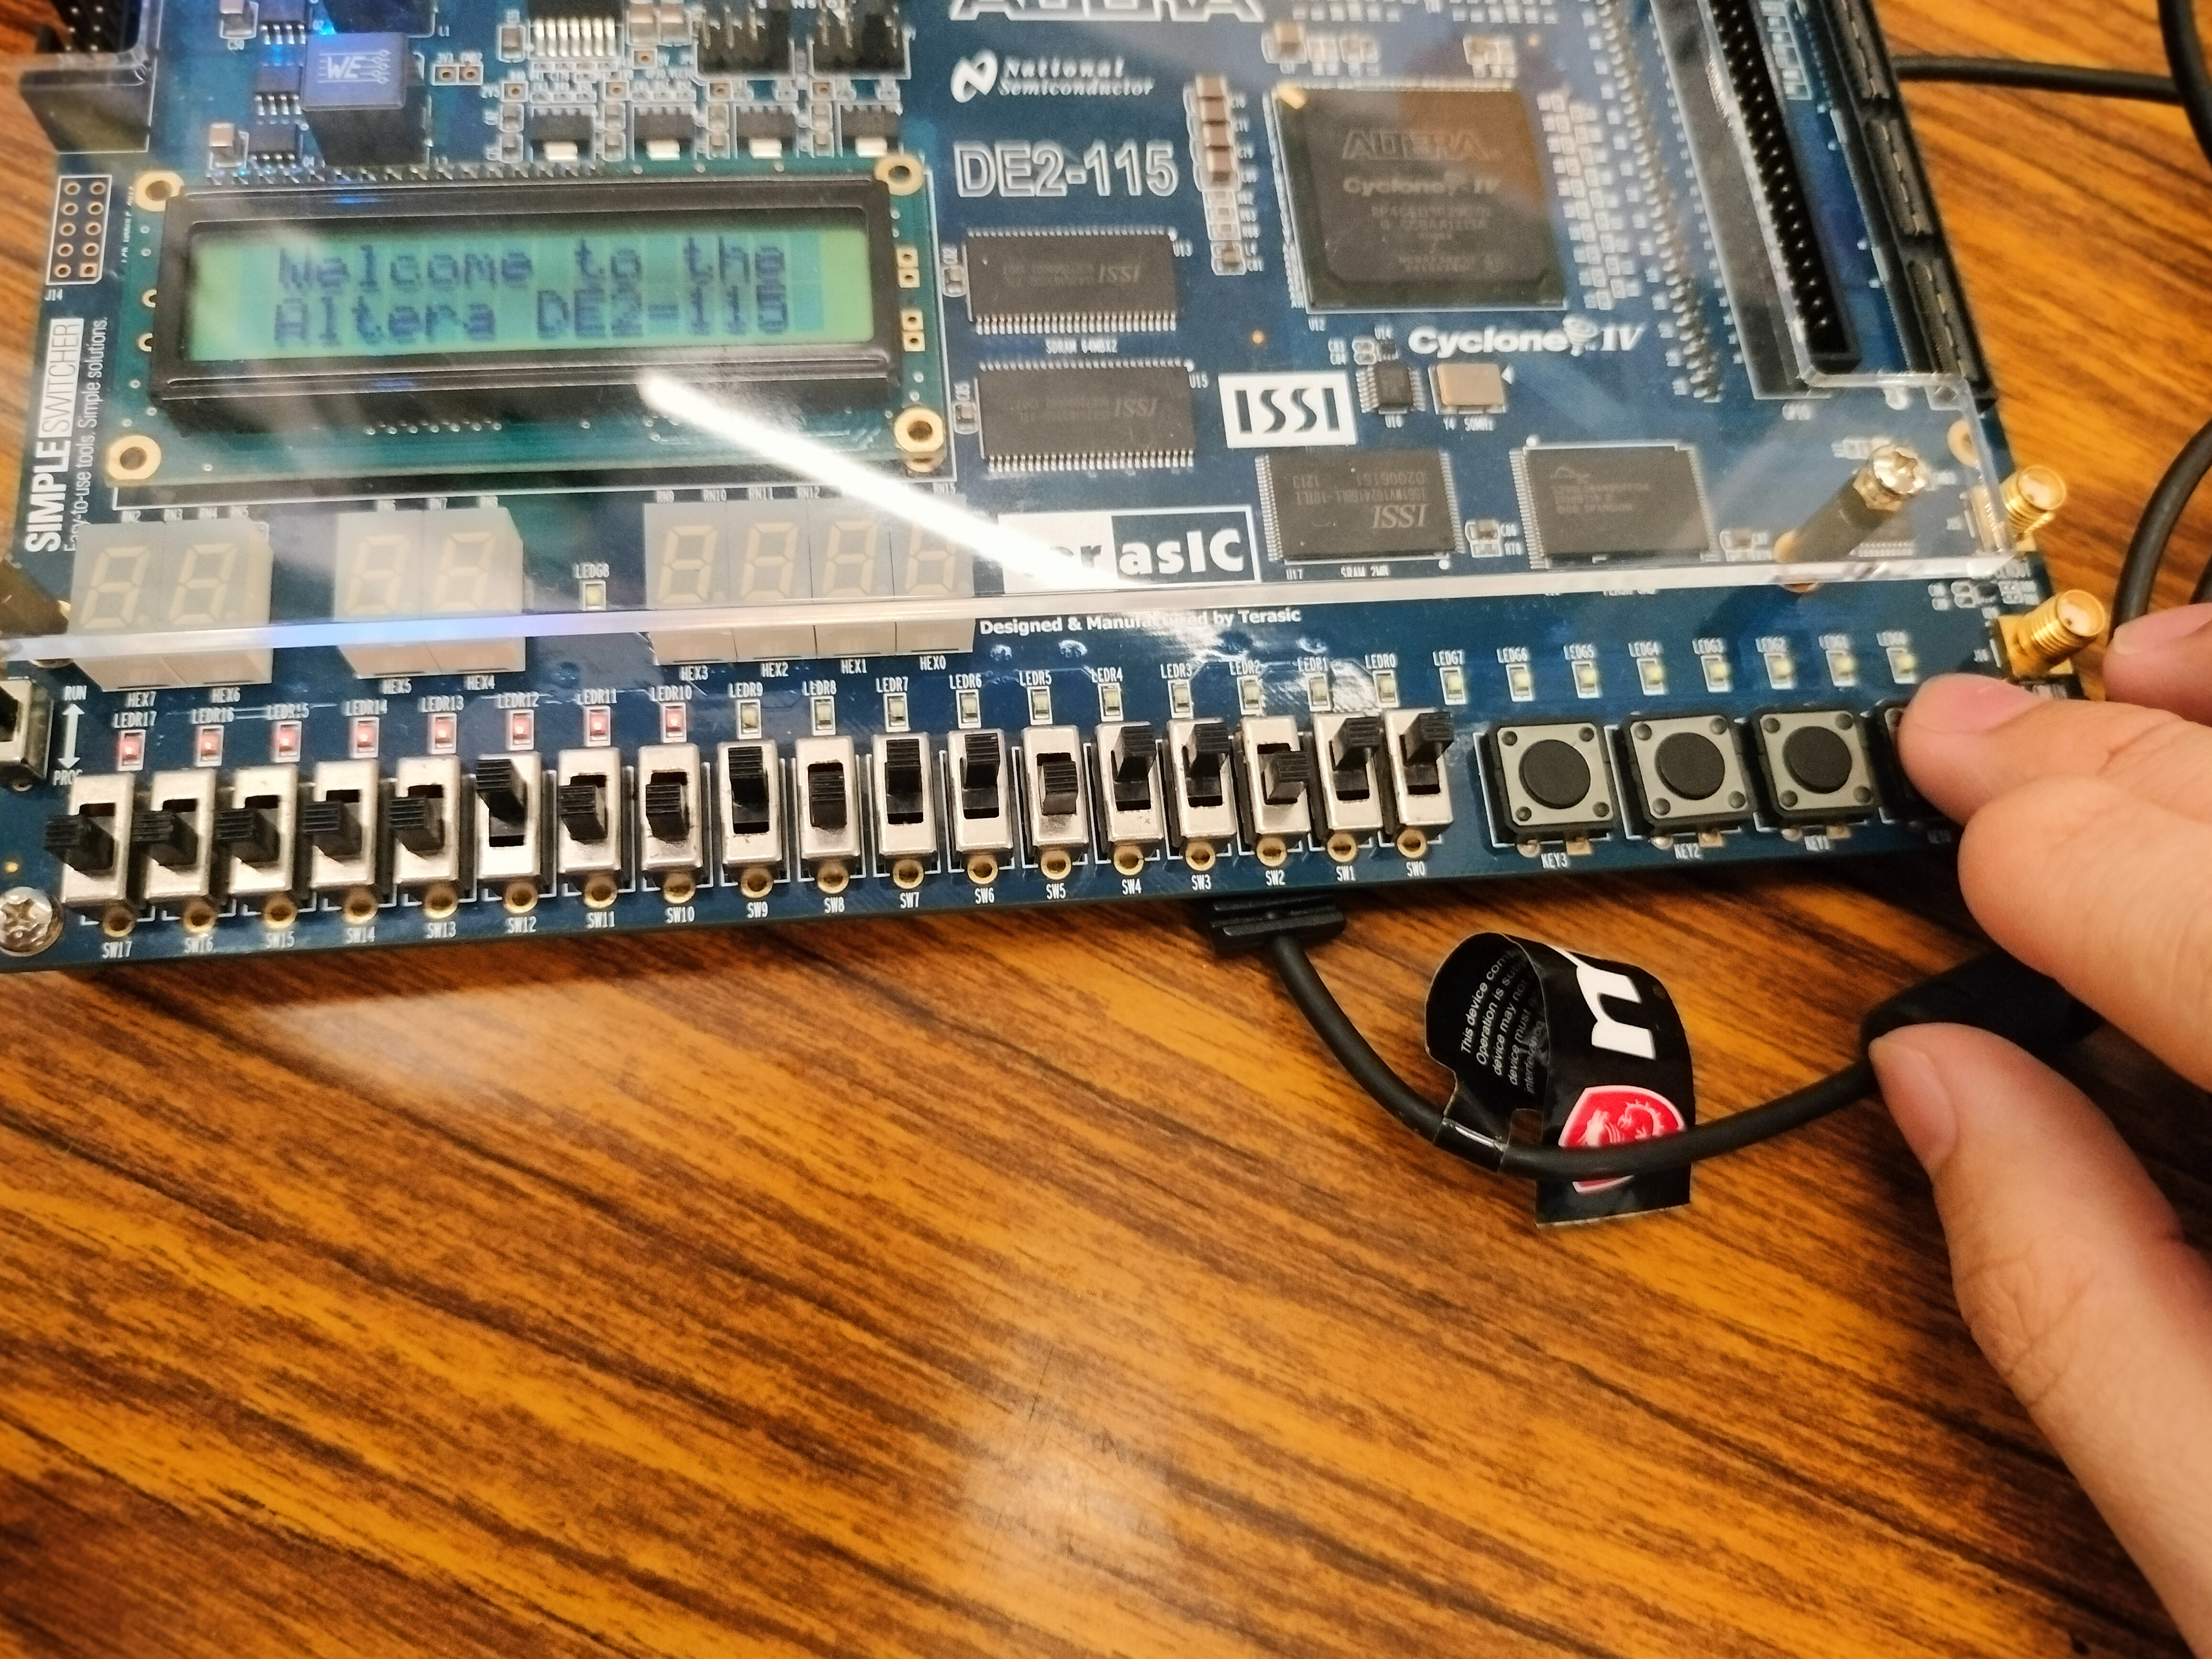
\includegraphics[width=0.5\textwidth]{./Photo/IMG20260513213833.jpg} \\
\textbf{位移序列 C}：展示連續位移的連貫性。 & 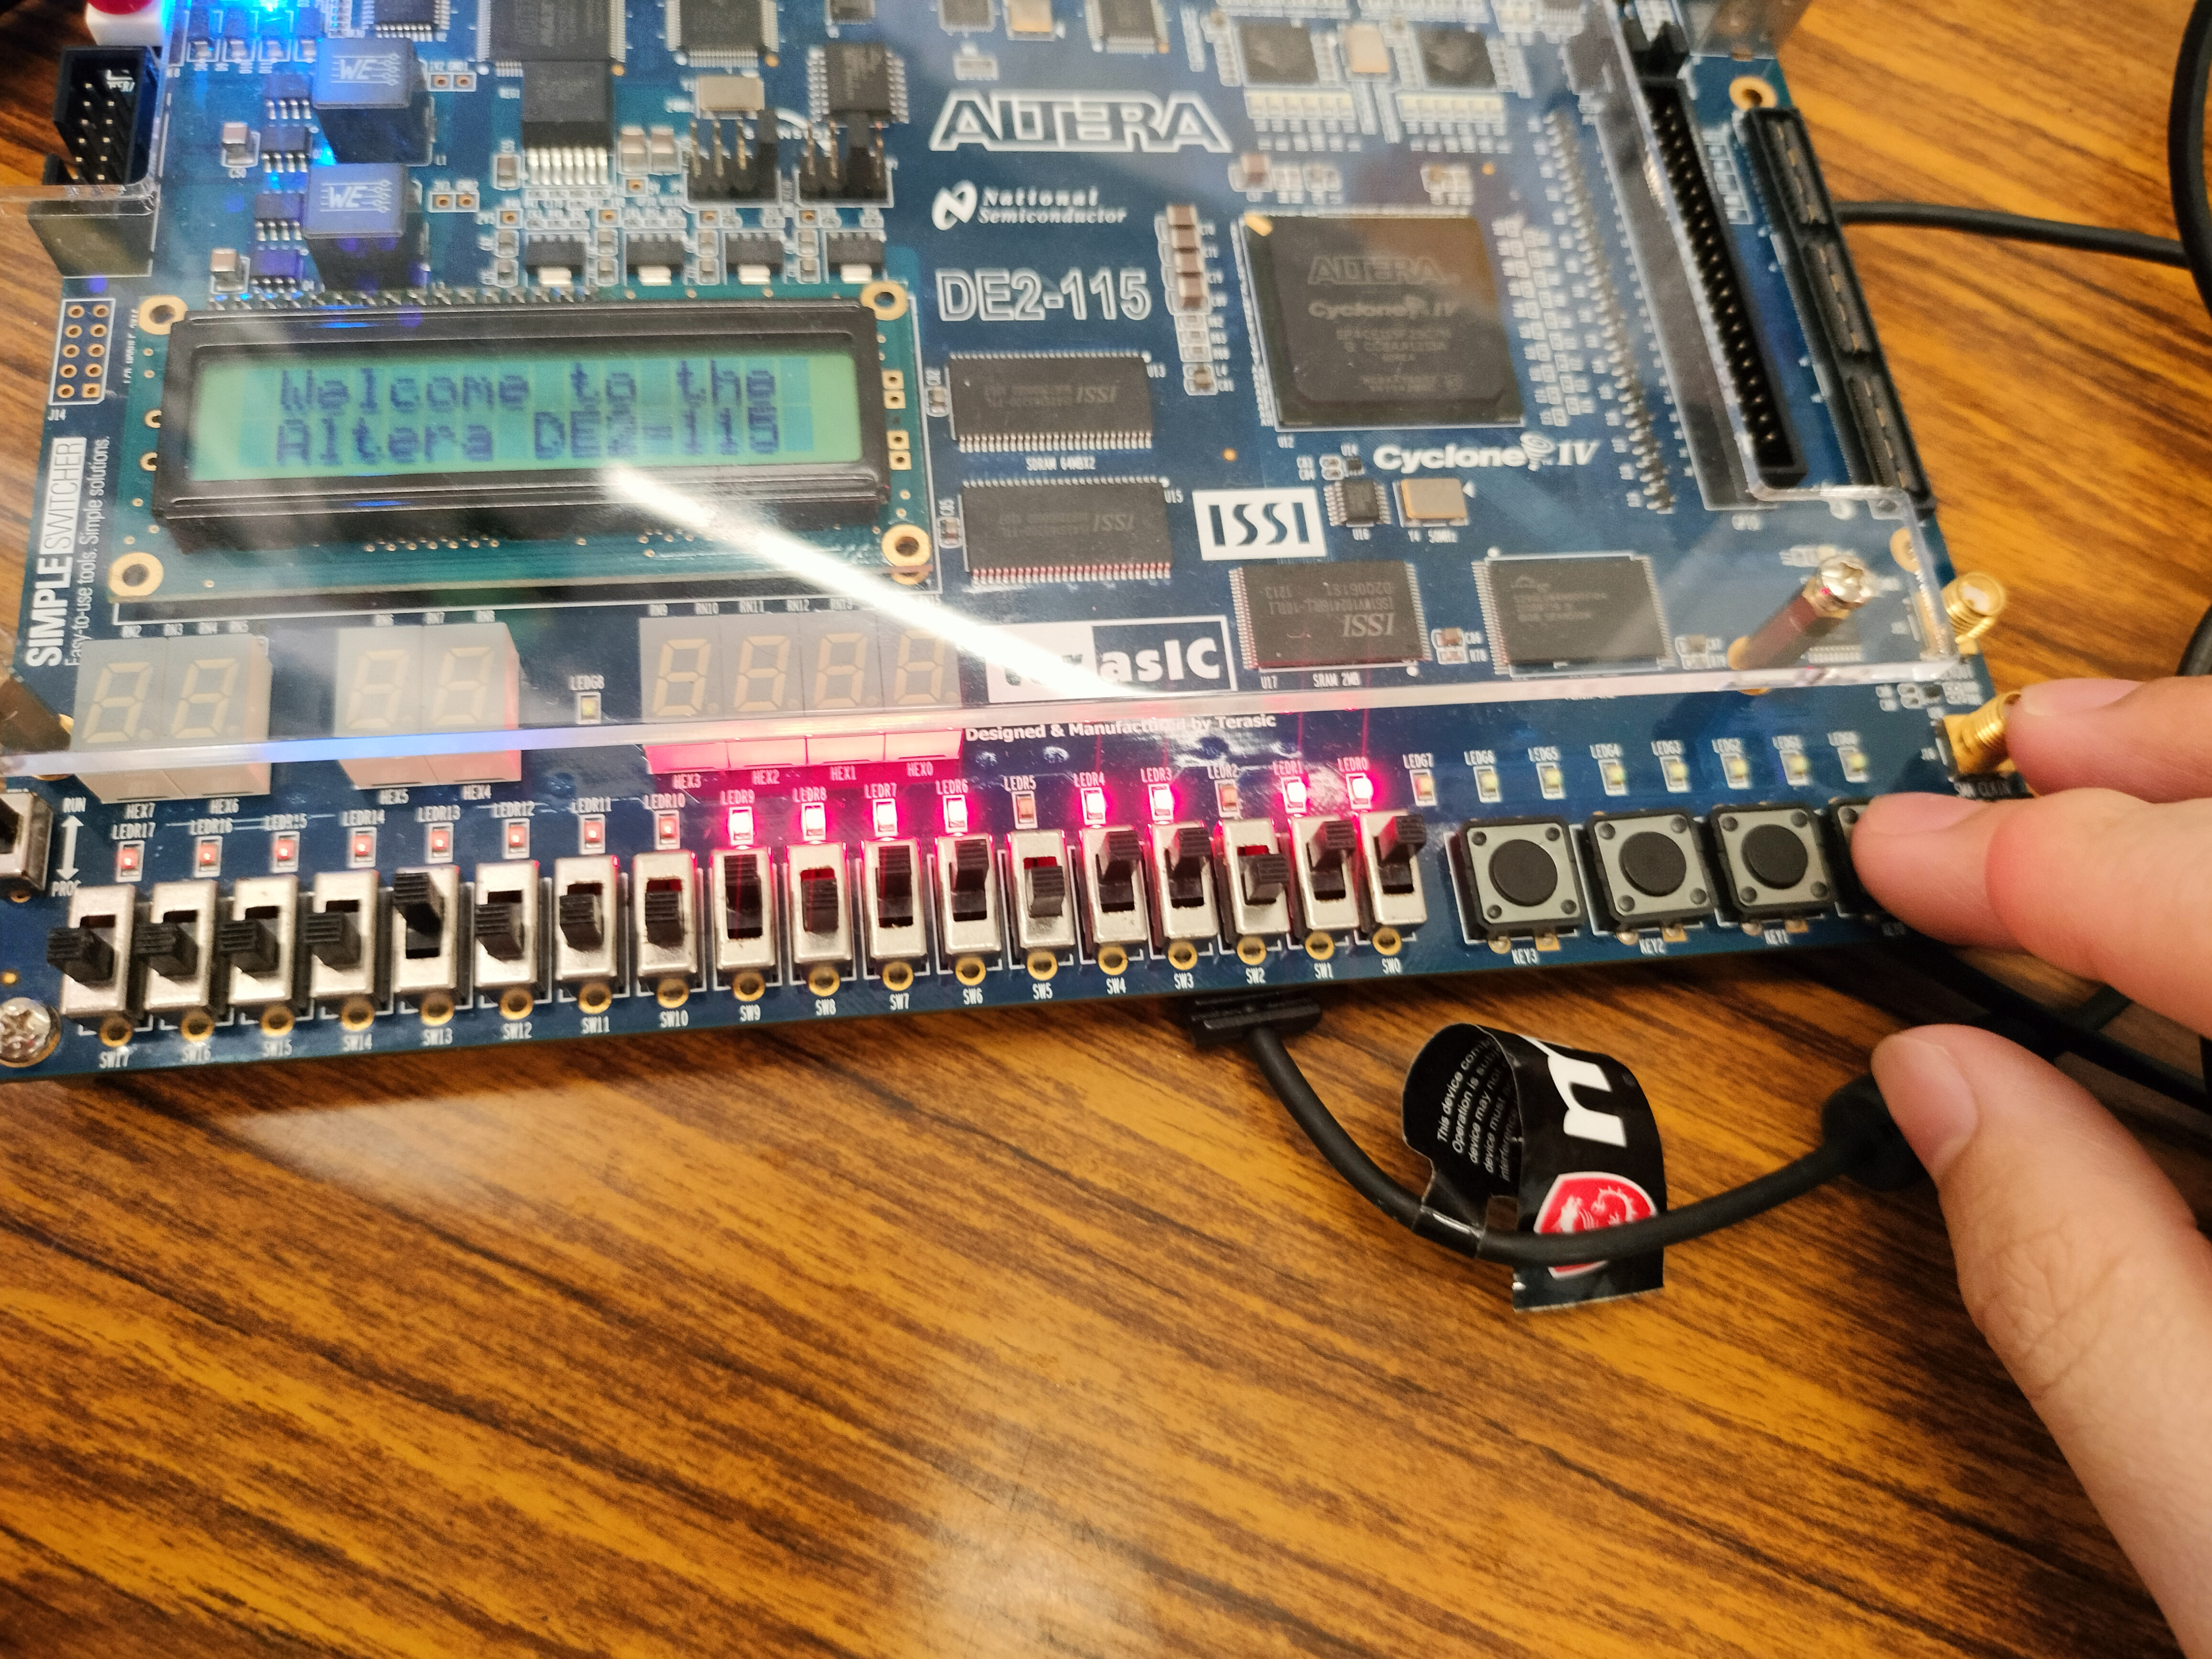
\includegraphics[width=0.5\textwidth]{./Photo/IMG20260513213859.jpg} \\
\bottomrule
\end{longtable}

\subsubsection{5. 右移操作 (Right Shift)}
\begin{longtable}{p{5cm} c}
\toprule
狀態描述 & 實體照片 \\
\midrule
\textbf{右移操作}：切換 SW11 (lr\_sel) 為 0，位元向右（低位元）移動。 & 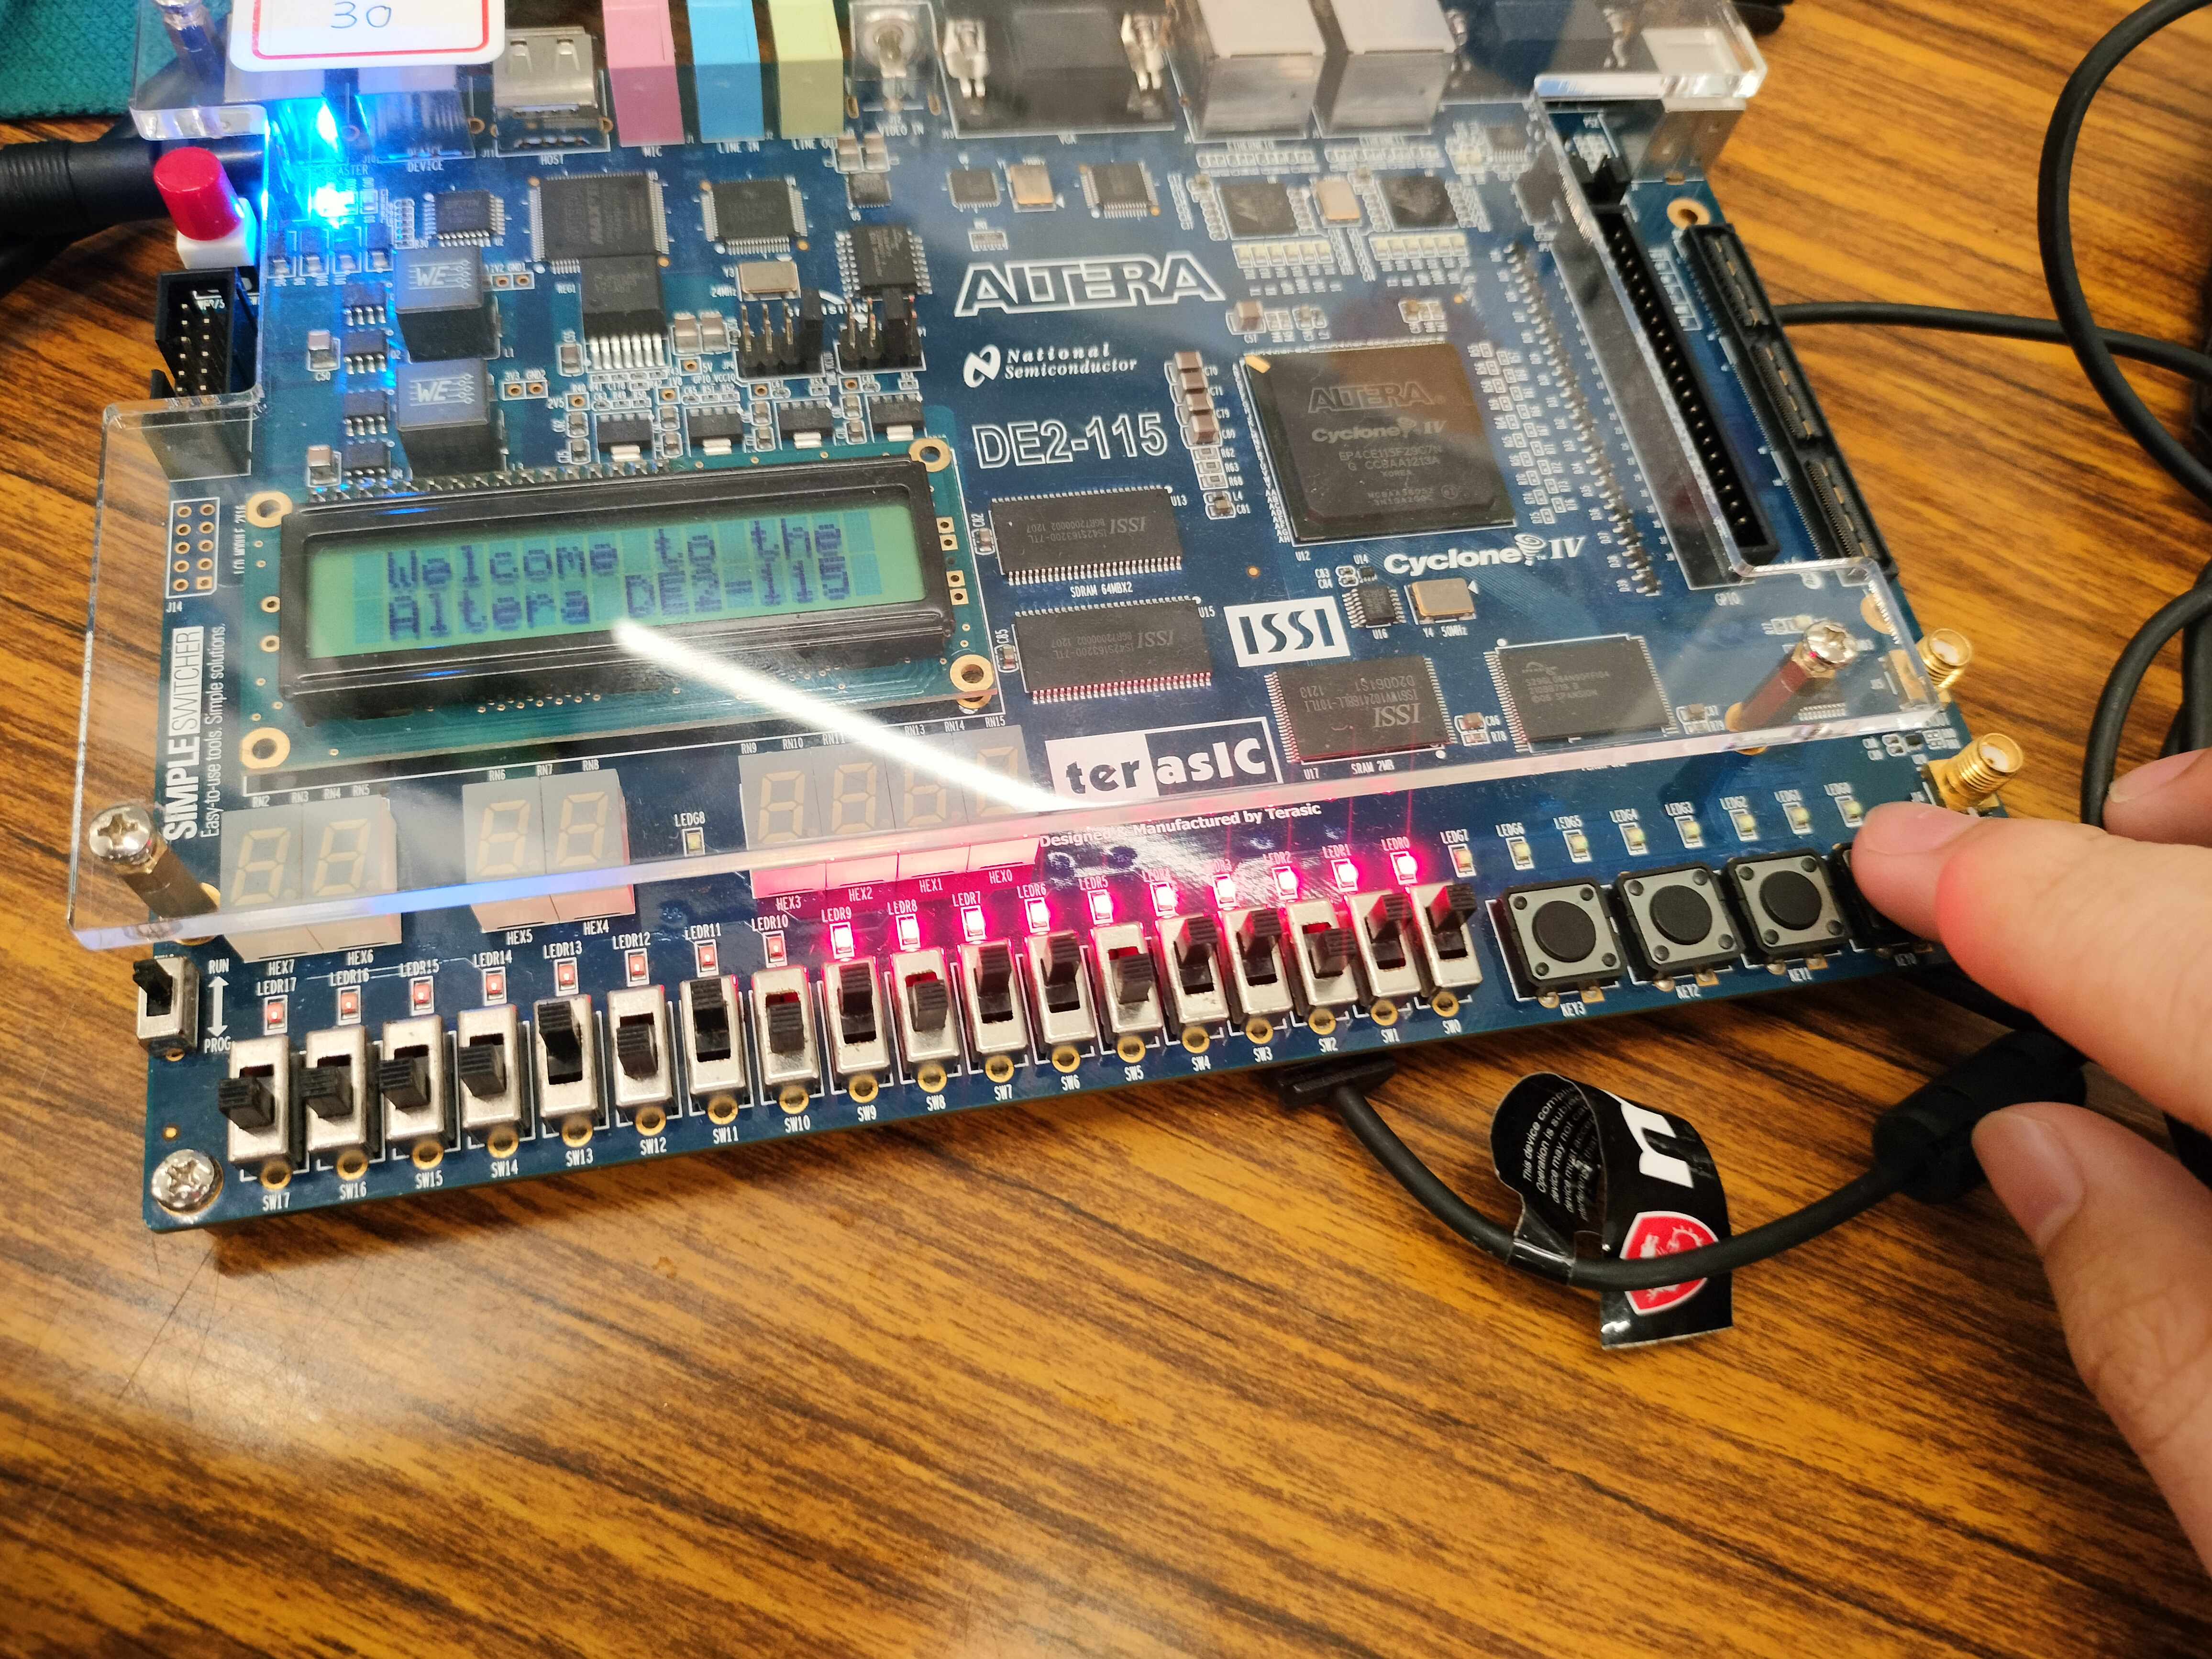
\includegraphics[width=0.5\textwidth]{./Photo/IMG20260513214908.jpg} \\
\textbf{右移至結束}：觀察數值逐位移向 LEDR0。 & 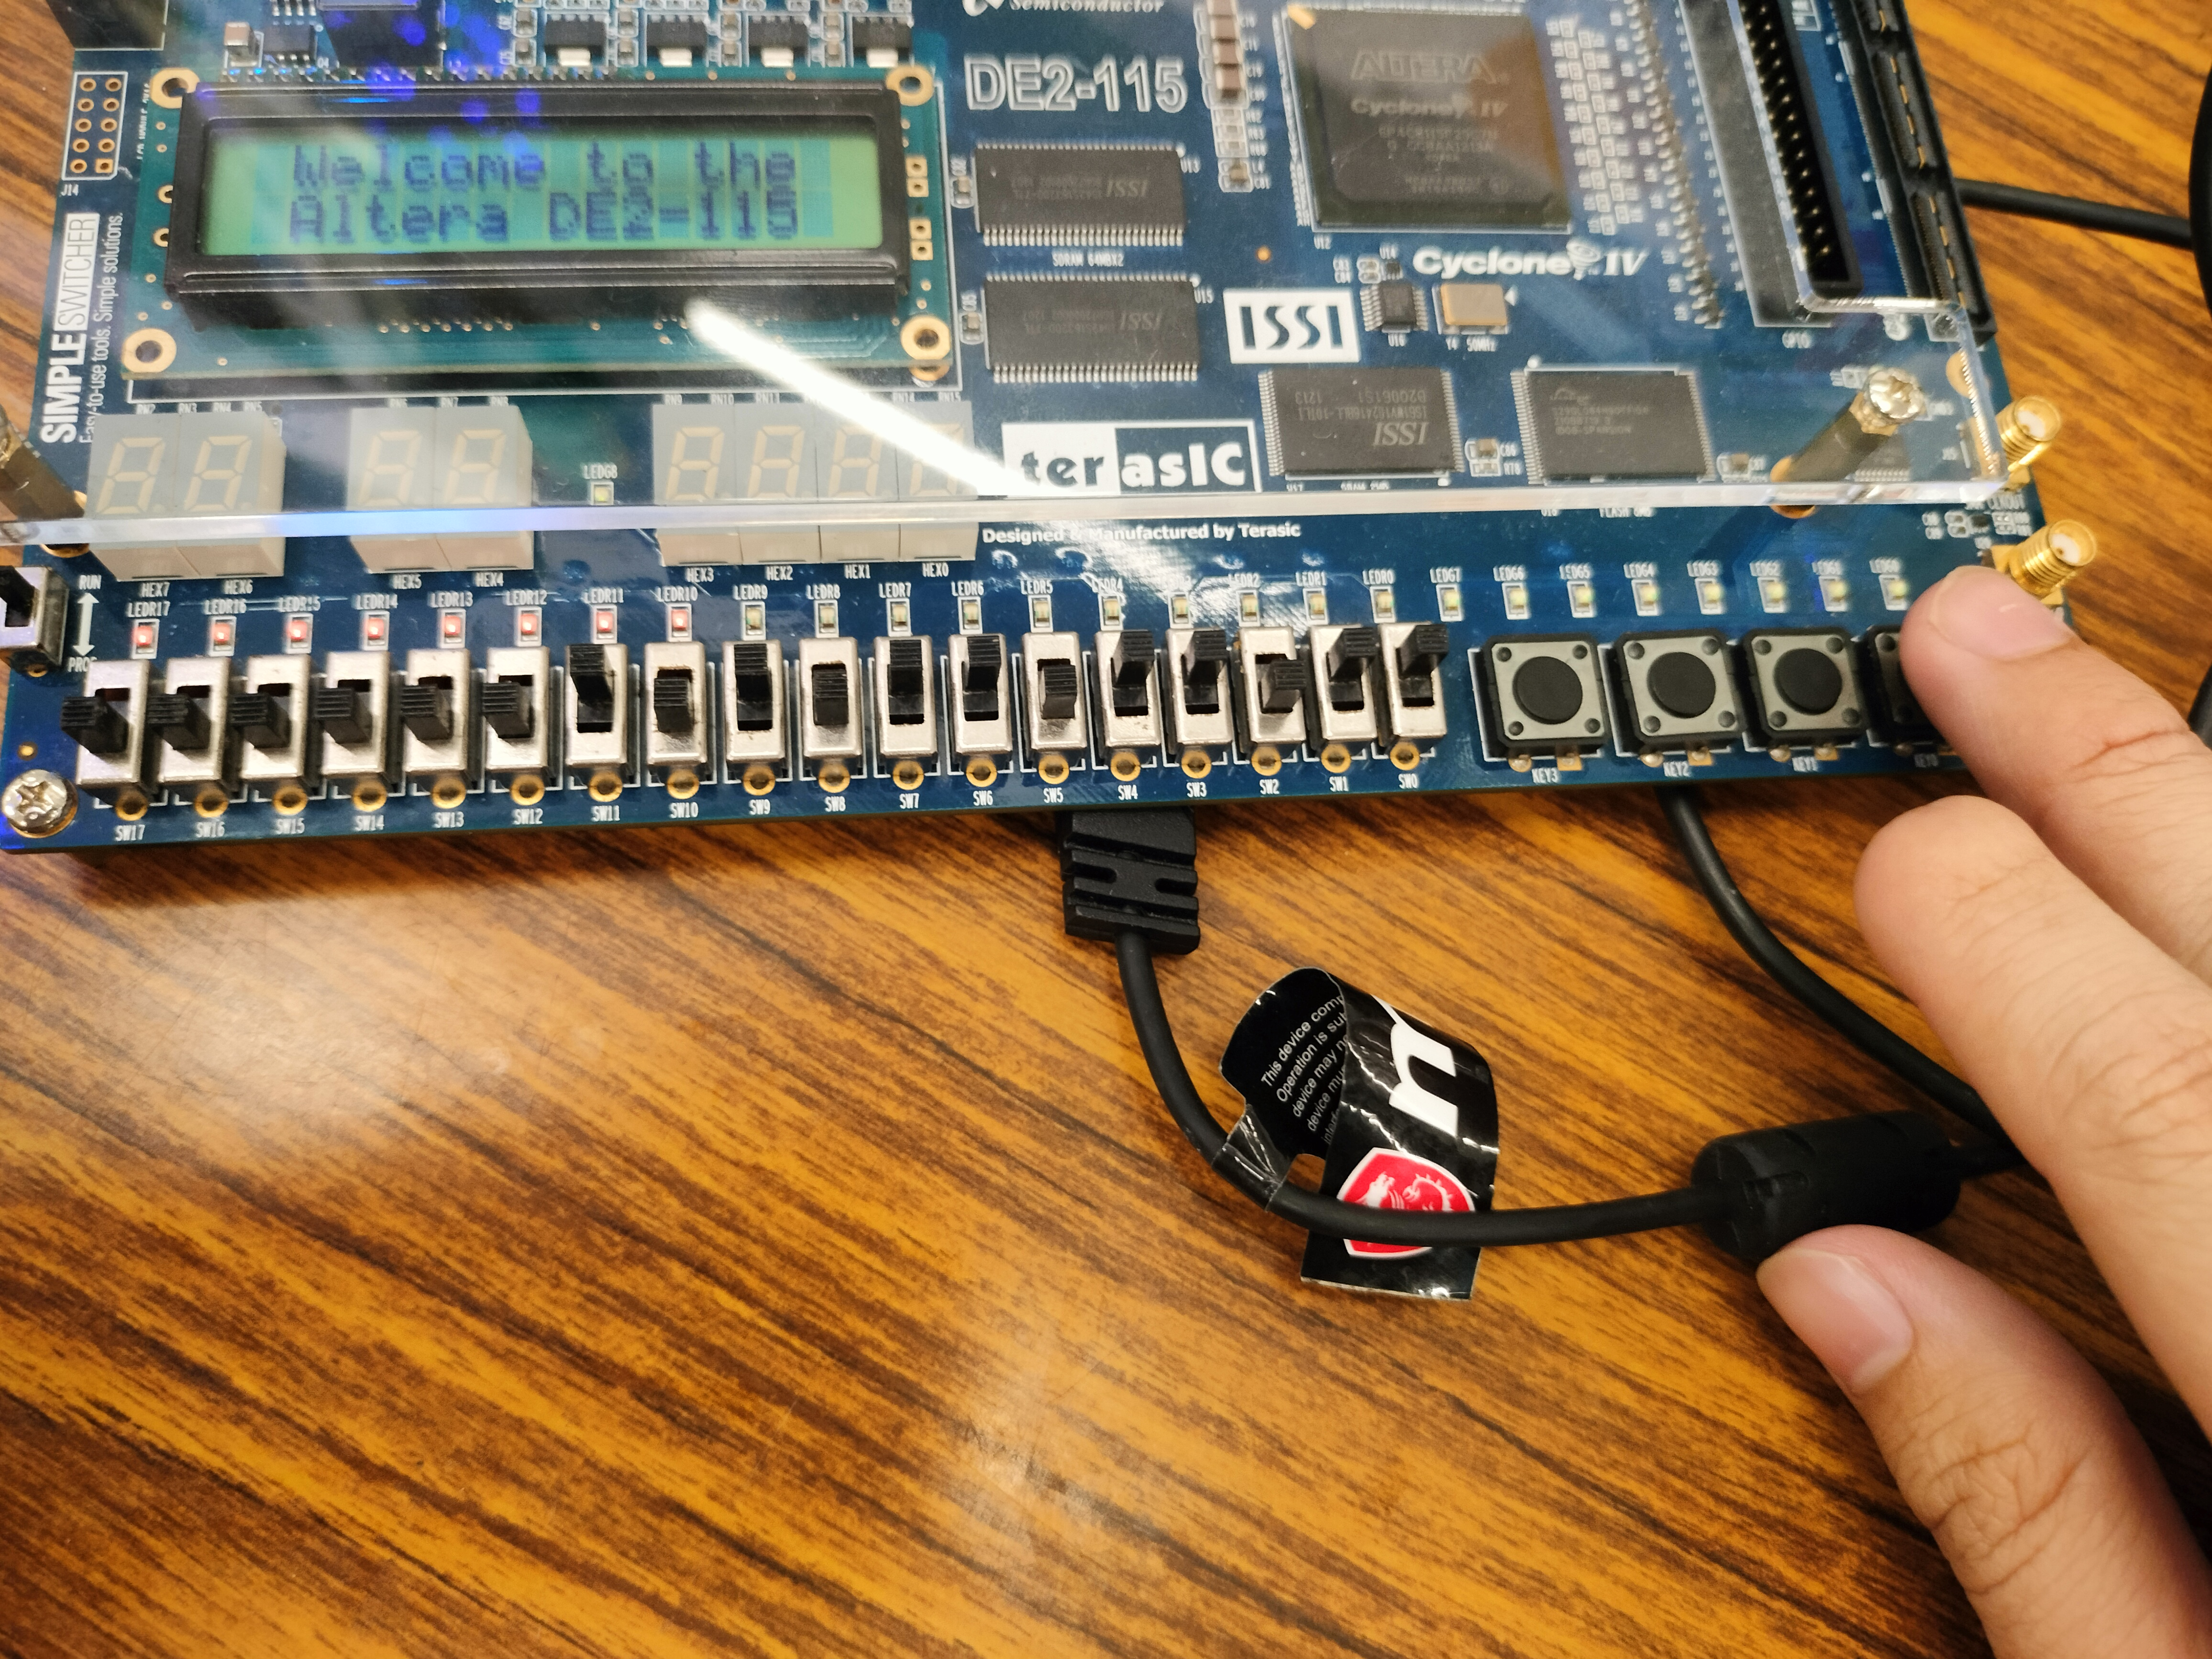
\includegraphics[width=0.5\textwidth]{./Photo/IMG20260513213448.jpg} \\
\bottomrule
\end{longtable}

\subsubsection{6. 更多實驗細節}
\begin{longtable}{p{5cm} c}
\toprule
狀態描述 & 實體照片 \\
\midrule
\textbf{載入模式細節 A}：特定開關組合下的輸出狀態。 & 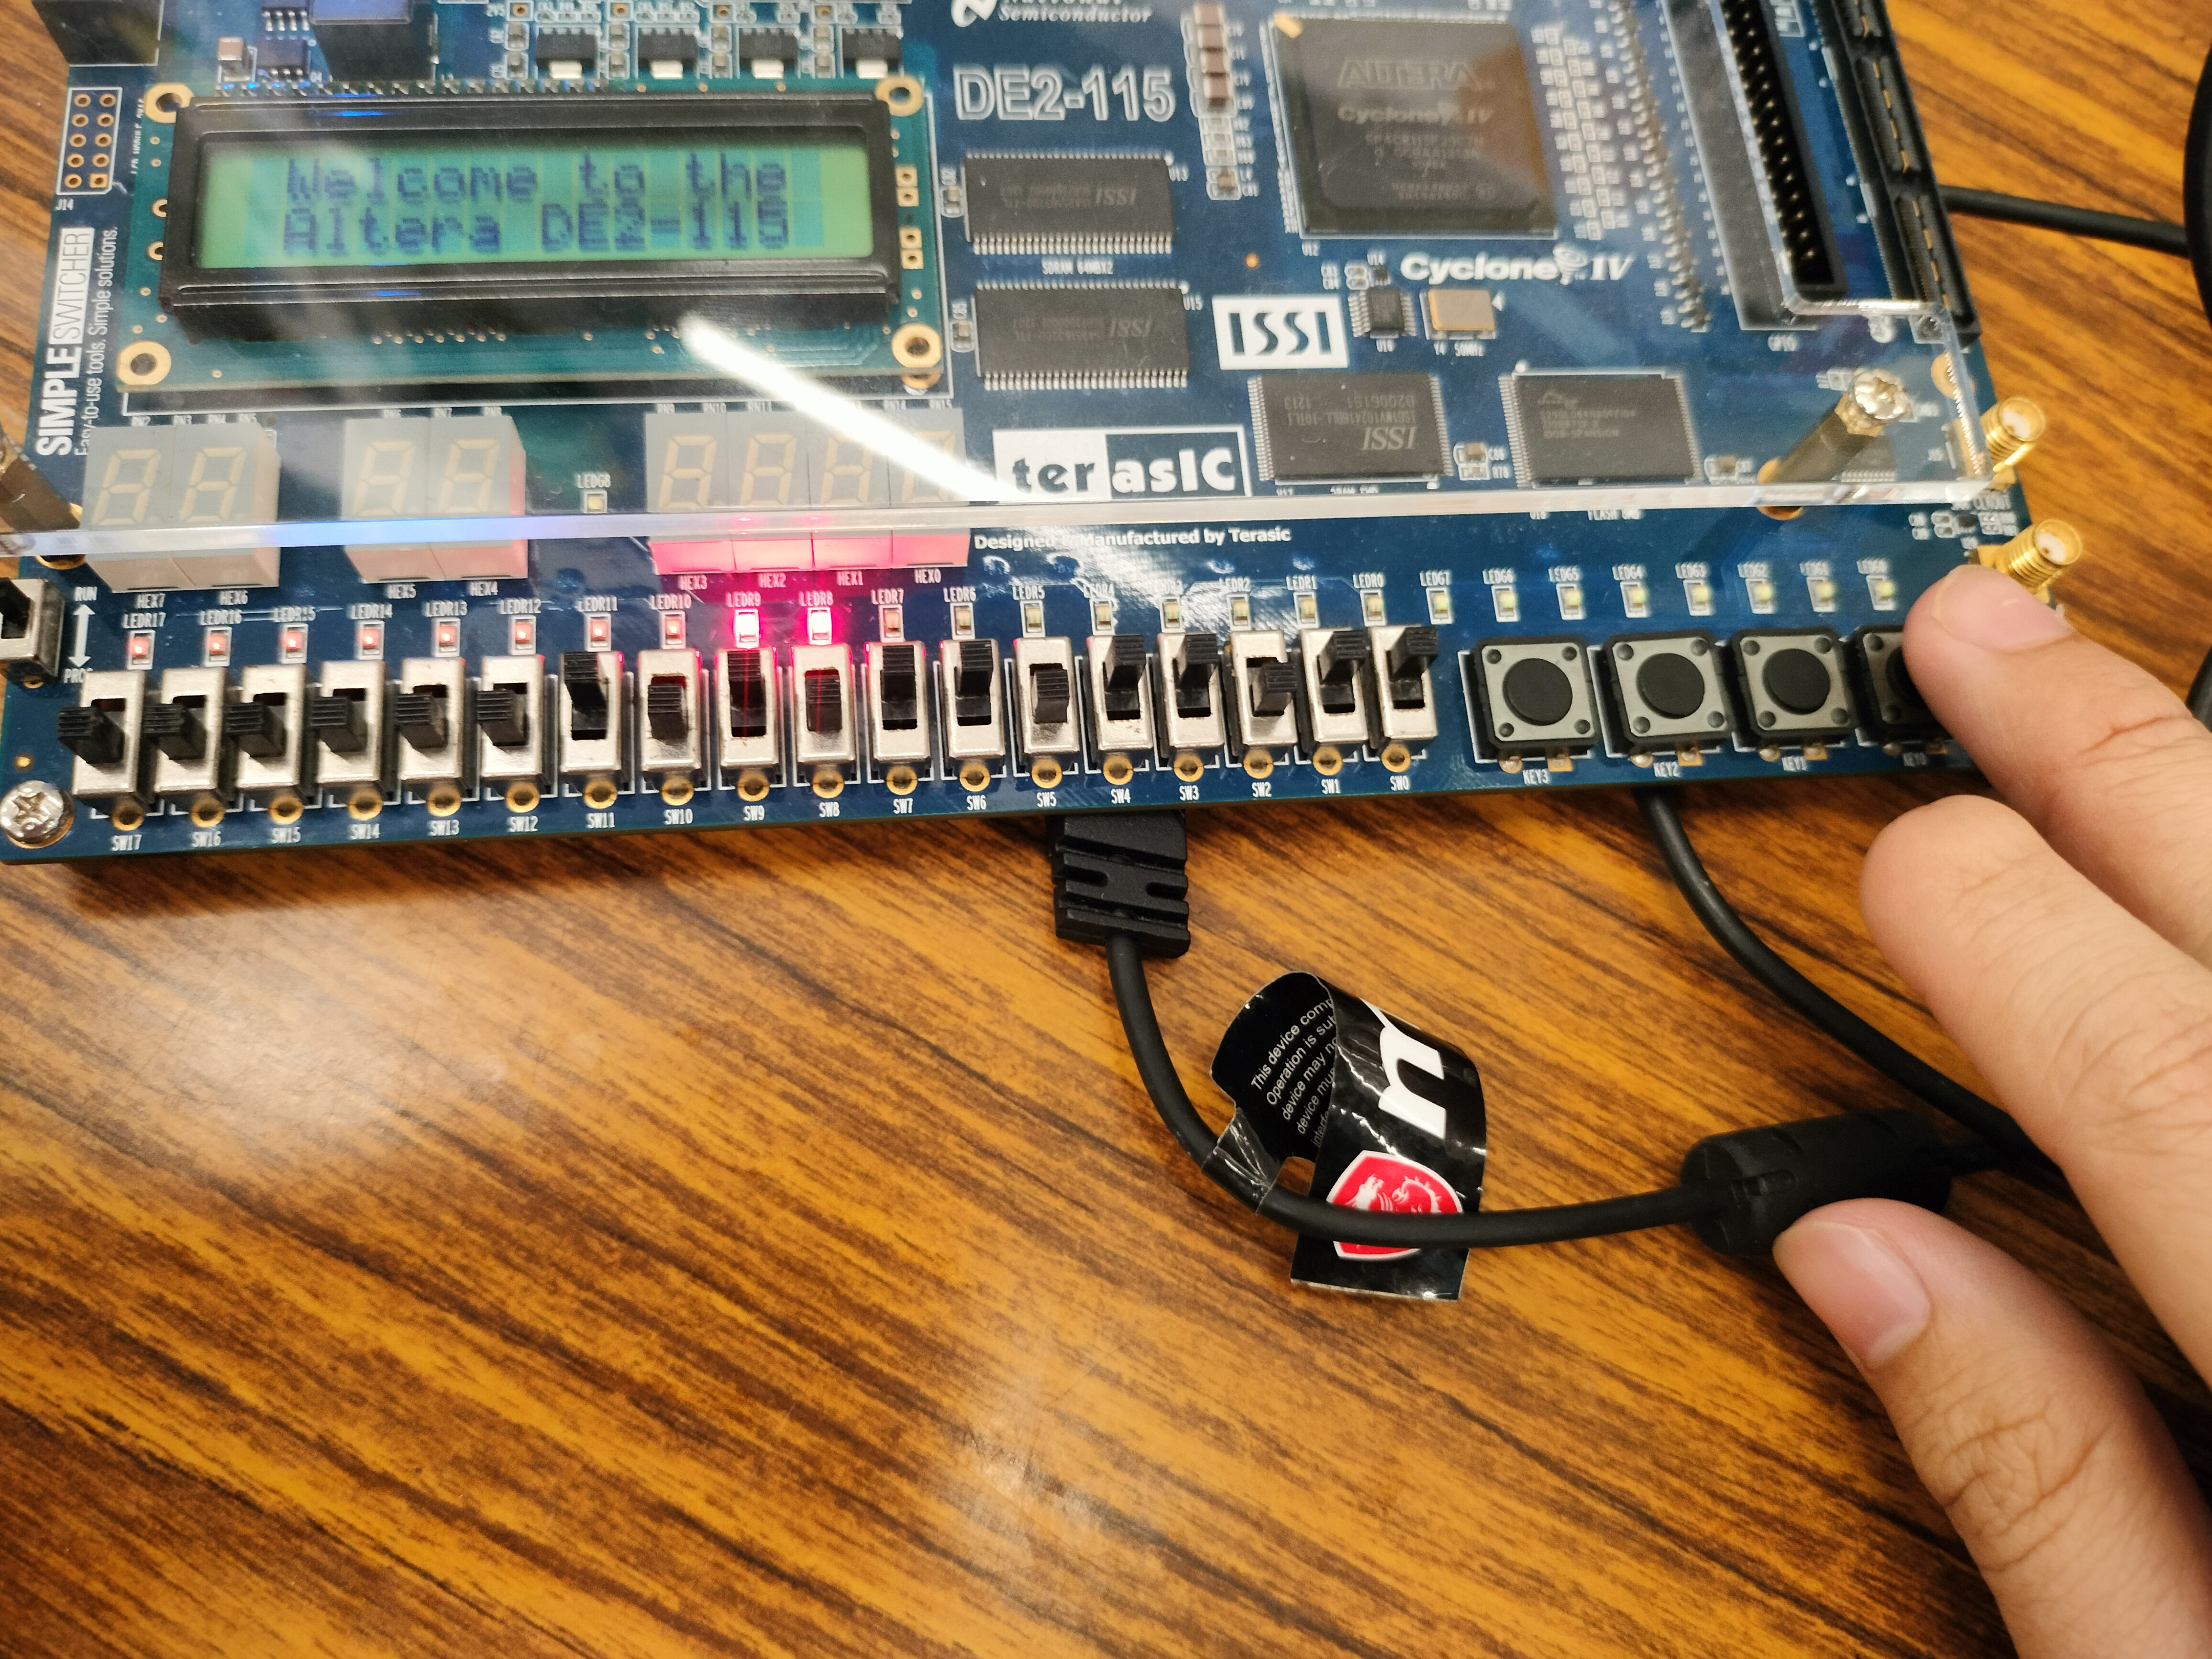
\includegraphics[width=0.5\textwidth]{./Photo/IMG20260513213443.jpg} \\
\textbf{載入模式細節 B}：特定開關組合下的輸出狀態。 & 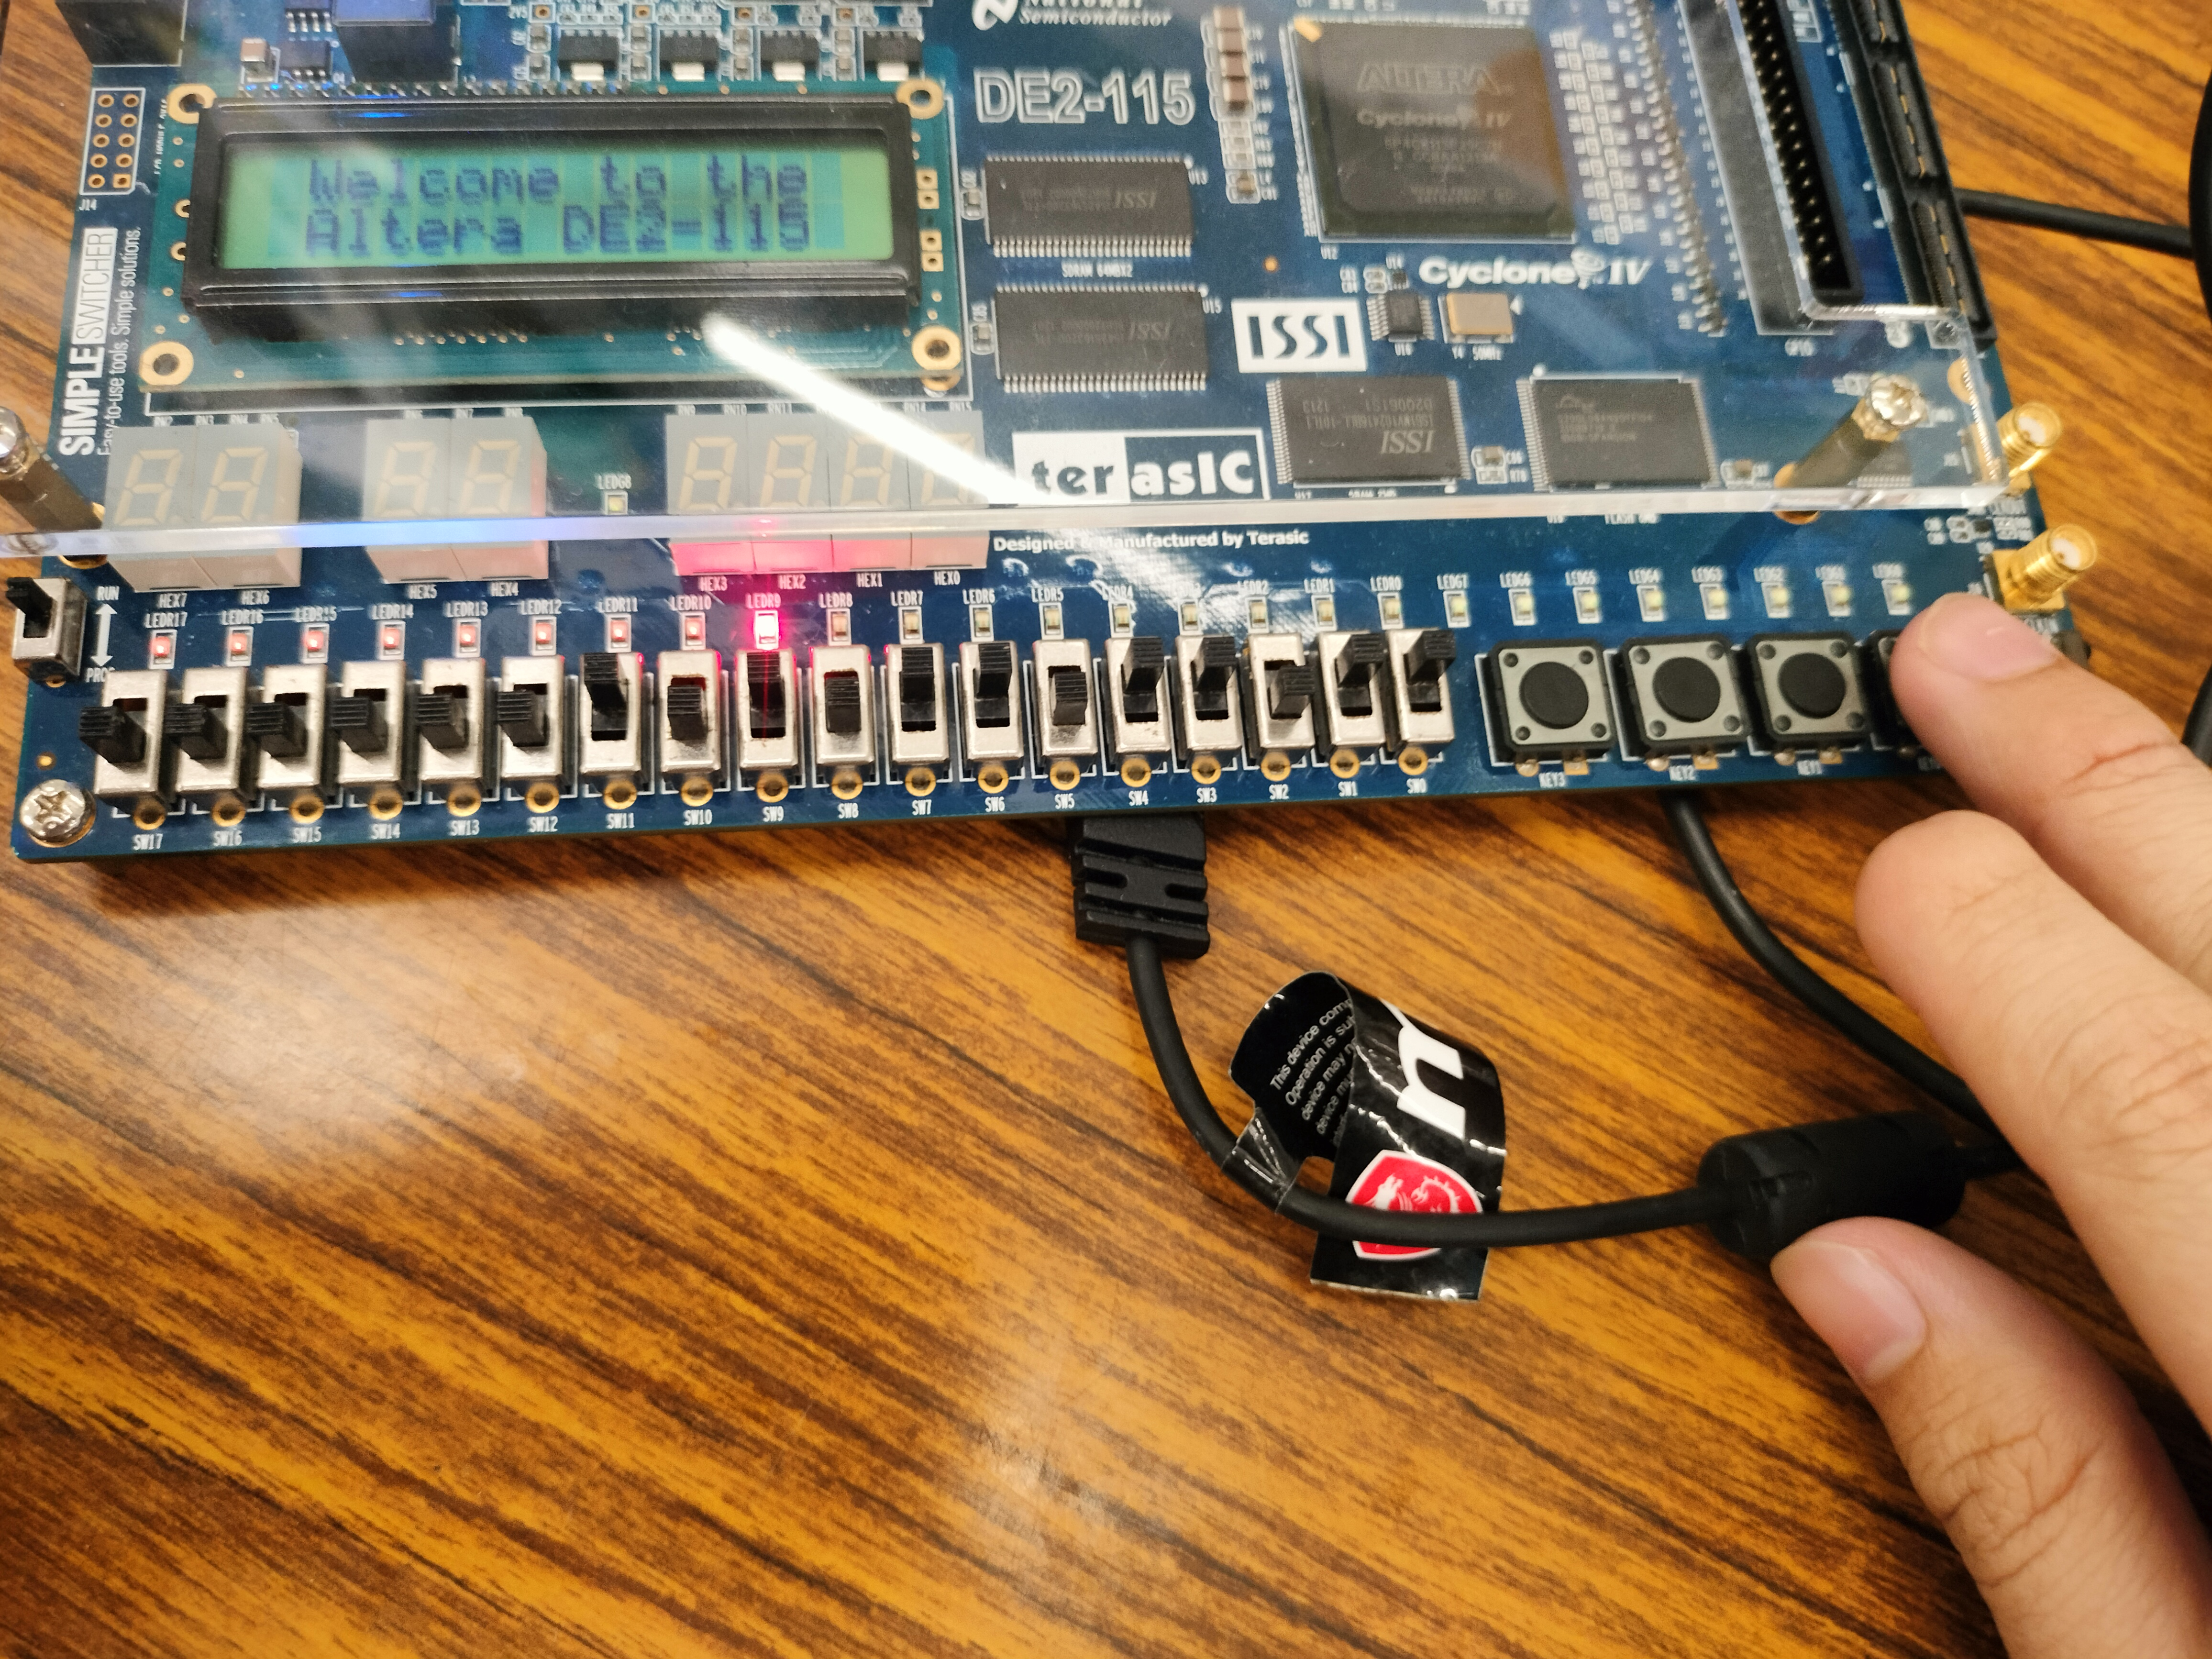
\includegraphics[width=0.5\textwidth]{./Photo/IMG20260513213446.jpg} \\
\textbf{位移中間態}：觀察位移過程中的 LED 變化。 & 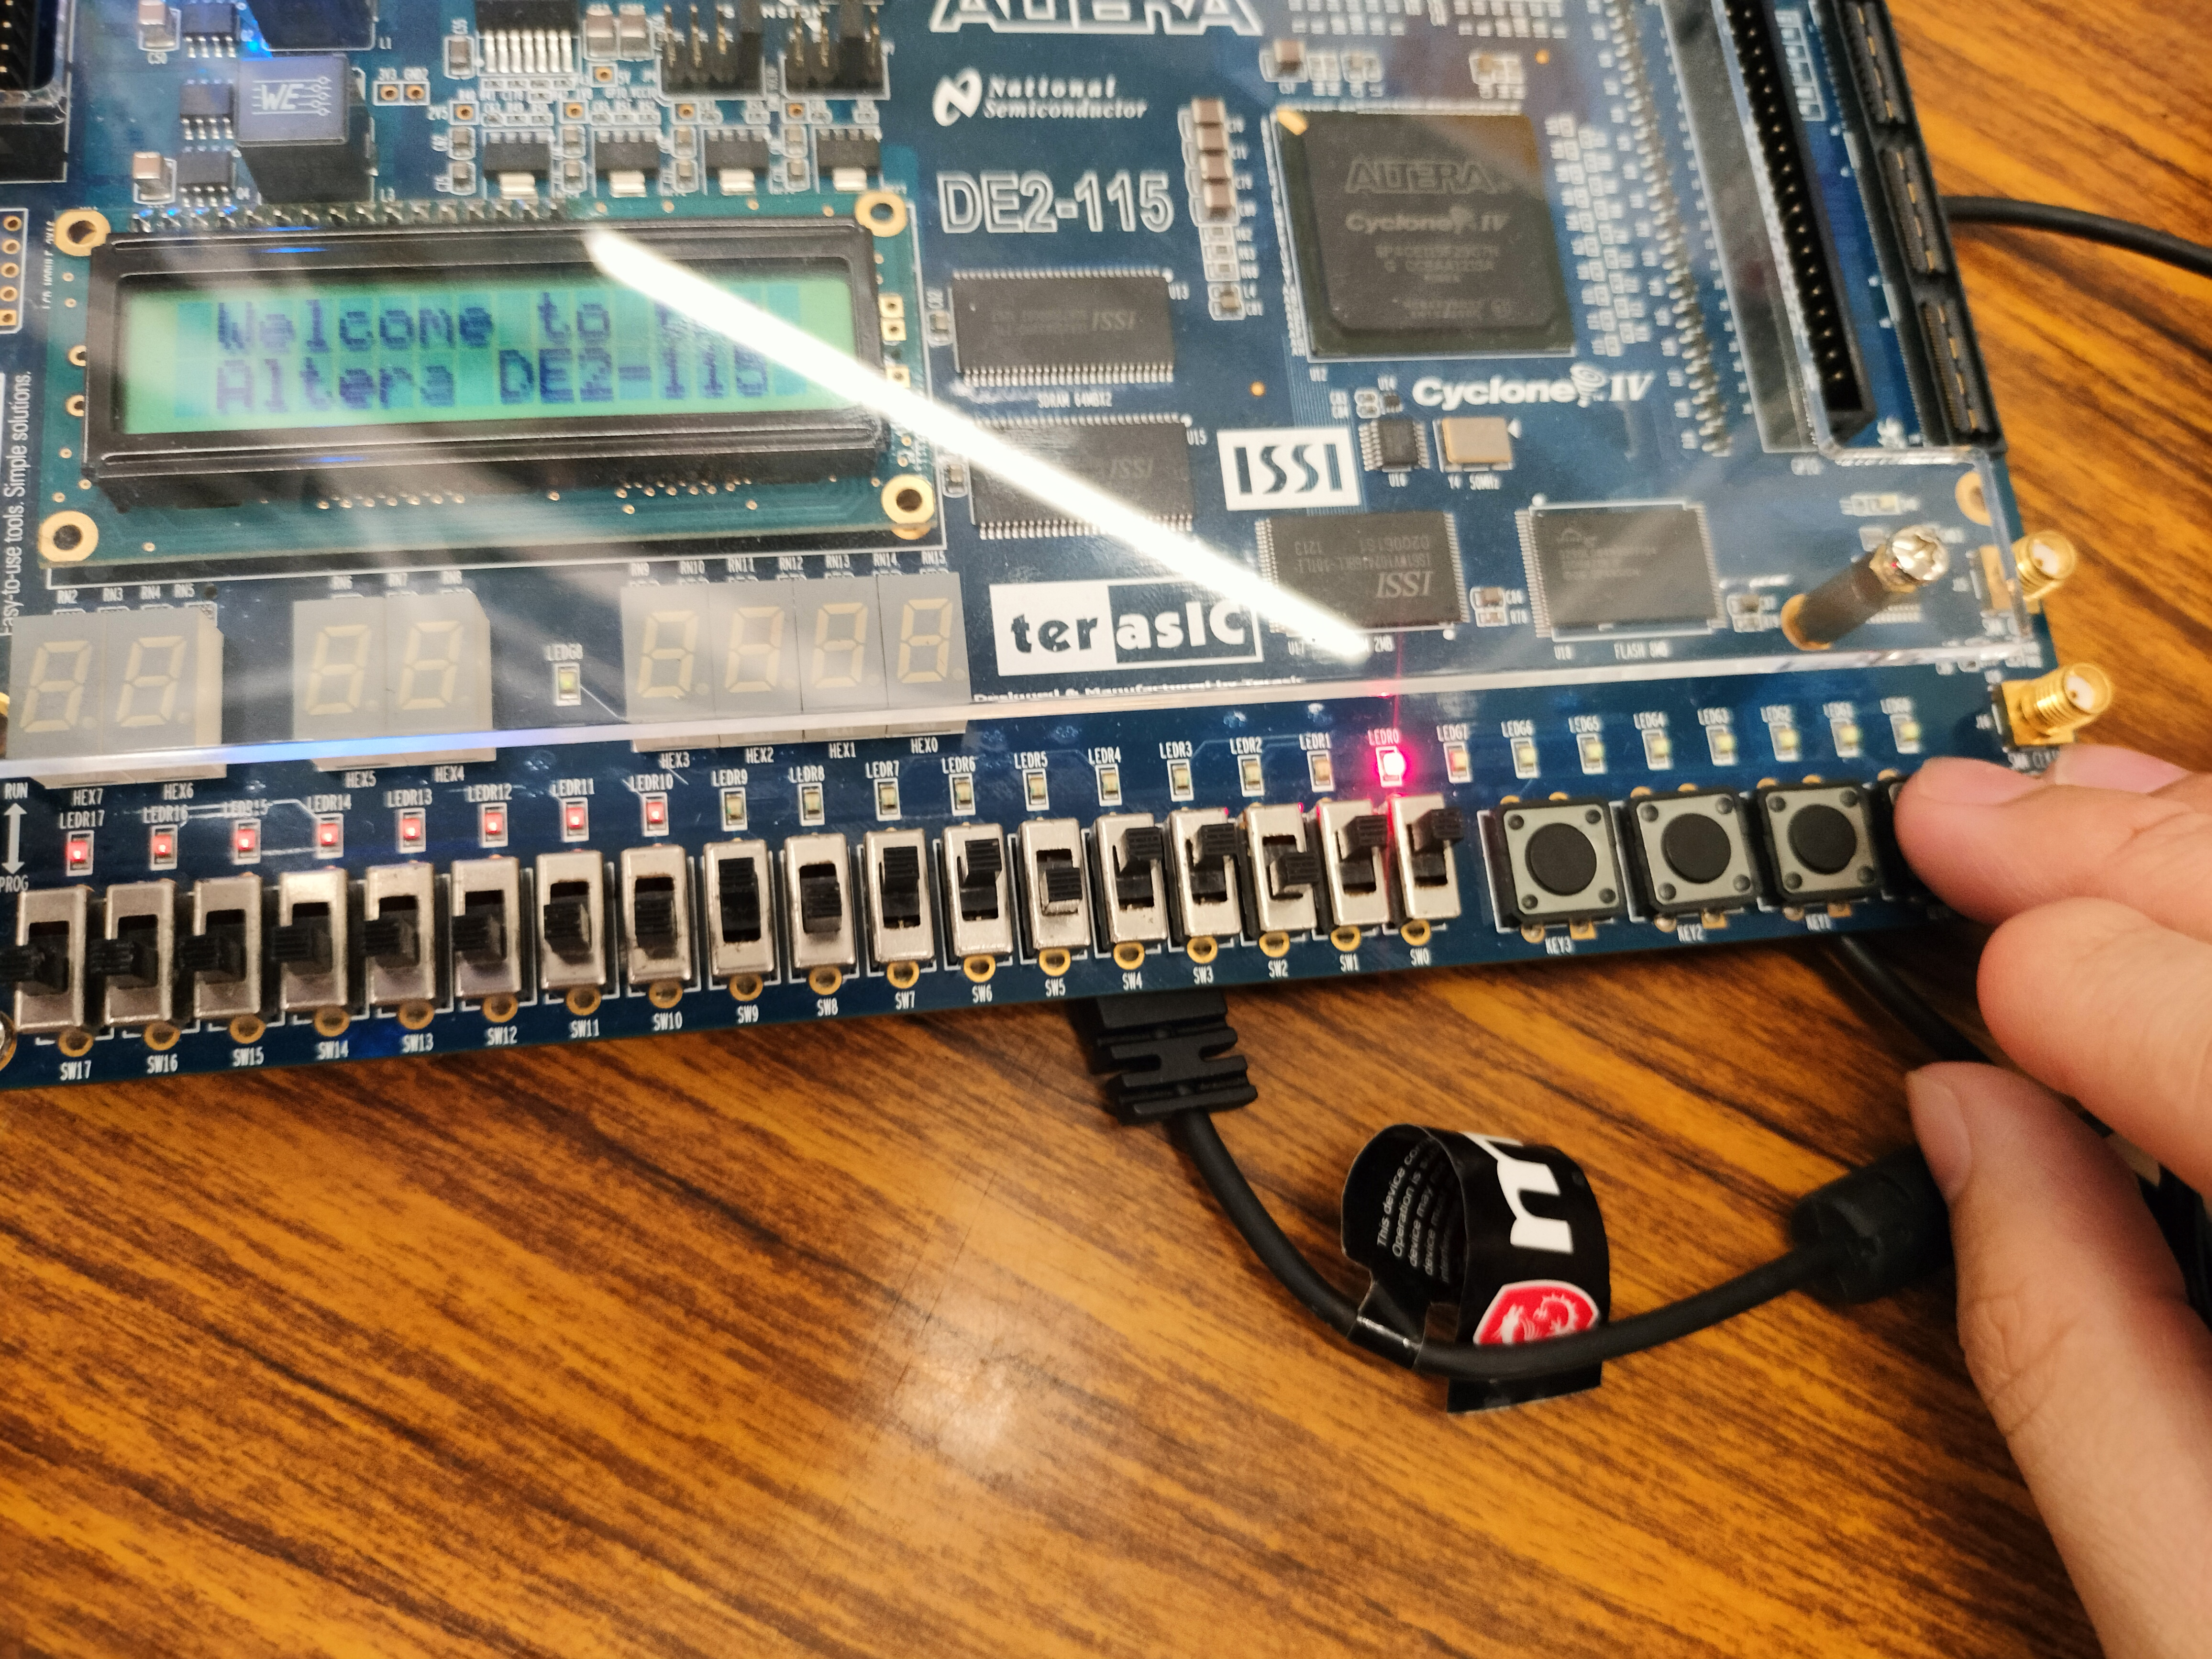
\includegraphics[width=0.5\textwidth]{./Photo/IMG20260513213759.jpg} \\
\bottomrule
\end{longtable}

\section{程式碼 (僅包含目標一：N\_bit\_DFF.vhd)}
\begin{lstlisting}[language=VHDL]
library ieee;
use ieee.std_logic_1164.all;
use ieee.std_logic_unsigned.all;

entity n_bit_DFF is
    generic( N : integer := 10 ); -- 使用 GENERIC 讓位元數可變
    port( 
        clk    : in  std_logic;
        clean  : in  std_logic;
        load   : in  std_logic;
        lr_sel : in  std_logic;
        di     : in  std_logic_vector(N-1 downto 0);
        sdi    : in  std_logic;
        qo     : out std_logic_vector(N-1 downto 0)
    );
end entity n_bit_DFF;

architecture Behavioral of n_bit_DFF is
    signal reg : std_logic_vector(N-1 downto 0) := (others => '0');
begin
    process(clk)
    begin
        if rising_edge(clk) then
            if clean = '1' then
                reg <= (others => '0');
            elsif load = '1' then
                reg <= di;
            elsif lr_sel = '1' then
                for i in N-1 downto 1 loop
                    reg(i) <= reg(i-1);
                end loop;
                reg(0) <= sdi;
            elsif lr_sel = '0' then
                for i in 0 to N-2 loop
                    reg(i) <= reg(i+1);
                end loop;
                reg(N-1) <= sdi;
            end if;
        end if;
    end process;
    qo <= reg;
end architecture Behavioral;
\end{lstlisting}

\section{實驗心得}
在本次 Lab 05 實驗中，我們學習了如何設計並實作一個多功能的萬用暫存器。這項實驗讓我們更深刻地理解了數位電路中「同步控制」的機制。與組合邏輯不同，序向邏輯（Sequential Logic）中的所有行為都依賴於時脈（Clock）的觸發，這在 VHDL 中透過 \texttt{rising\_edge(clk)} 來精準控制。

特別是在處理左移與右移邏輯時，我們使用了 \texttt{for loop} 迴圈來撰寫。雖然在硬體實現上，迴圈會被展開成平行排列的連線與多工器，但在撰寫程式碼時，這種方式極大地提高了可讀性與擴充性。此外，透過硬體開發板的實作，我們觀察到當 \texttt{clean} 或 \texttt{load} 訊號為高電位時，必須按下 \texttt{KEY0} 提供時脈緣，暫存器的狀態才會更新。這讓我們學會區分「準位觸發」與「邊緣觸發」的差異。整體而言，這次實驗讓我們對暫存器在計算機系統中扮演的角色有了更紮實的認識。

\section{組員貢獻比例}
\begin{table}[H]
\centering
\begin{tabular}{@{}llll@{}}
\toprule
姓名 & 學號 & 貢獻比例 & 負責內容 \\
\midrule
楊承諭 & 113590051 & 100\% & 程式開發、硬體測試、影像紀錄、報告撰寫 \\
黃楷程 & 113590017 & 0\% & 無 \\
\bottomrule
\end{tabular}
\end{table}

\end{document}
